% This LaTeX document needs to be compiled with XeLaTeX.
\documentclass[10pt]{article}
\usepackage[utf8]{inputenc}
\usepackage{hyperref}
\hypersetup{colorlinks=true, linkcolor=blue, filecolor=magenta, urlcolor=cyan,}
\urlstyle{same}
\usepackage{amsmath}
\usepackage{amsfonts}
\usepackage{amssymb}
\usepackage[version=4]{mhchem}
\usepackage{stmaryrd}
\usepackage{graphicx}
\usepackage[export]{adjustbox}
\graphicspath{ {./images/} }
\usepackage[fallback]{xeCJK}
\usepackage{polyglossia}
\usepackage{fontspec}
\setCJKmainfont{Noto Serif CJK TC}

\setmainlanguage{polish}
\setmainfont{CMU Serif}

\title{KURS KORESPONDENCYJNY MATEMATYKA }

\author{Tadeusz Inglot}
\date{}


\begin{document}
\maketitle


Zbiór zadań 1999-2004

Recenzenci\\
Rościsław RABCZUK\\
Zbigniew ROMANOWICZ

Opracowanie redakcyjne\\
Alina KACZAK

\section*{Projekt okładki}
Zofia i Dariusz GODLEWSCY\\
(O) Copyright by Oficyna Wydawnicza Politechniki Wroclawskiej, Wroclaw 2005

OFICYNA WYDAWNICZA POLITECHNIKI WROCLAWSKIEJ Wybrzeże Wyspiańskiego 27, 50-370 Wrocław

ISBN 83-7085-871-6

Drukarnia Oficyny Wydawniczej Politechniki Wroclawskiej. Zam. nr 403/2005.

\section*{SPIS TREŚCI}
\begin{enumerate}
  \item Przedmowa ..... 5
  \item Zadania ..... 7
  \item Indeks tematyczny ..... 57
  \item Odpowiedzi do zadań ..... 65
  \item Wskazówki do zadań ..... 97
  \item 12 przykładowych rozwiązań ..... 135
\end{enumerate}

\section*{Przedmowa}
Zbiór obejmuje zadania Korespondencyjnego Kursu z Matematyki z lat 19992004. Kurs ten jest prowadzony przez Instytut Matematyki Politechniki Wrocławskiej. Jest kontynuacja Korespondencyjnego Kursu Przygotowawczego z Matematyki, który w latach 1972-1999 był prowadzony wspólnie z Instytutem Matematyki Politechniki Warszawskiej.

Opracowując niniejszy zbiór, autor pragnął ułatwić szerokiemu gronu maturzystów i kandydatów na studia dostęp do materiałów kursu ujętych w wygodną, zwarta formę i w ten sposób pomóc im w lepszym opanowaniu wiadomości z matematyki w zakresie szkoły średniej oraz dać jeszcze jedną okazję do powtórzenia materiału.

Większość zadań jest oryginalna, część pochodzi z egzaminów wstępnych na Politechnikę Wrocławska z ostatnich 20 lat, a tylko niewielka liczba z innych źródeł (w tym powtórzenia zadań z lat ubiegłych). Dla udogodnienia samodzielnej pracy i zachęcenia do korzystania z tego zbioru, podano odpowiedzi, a w oddzielnym rozdziale także wskazówki do wszystkich zadań. W końcowej części zbioru przedstawiono 12 przykładowych rozwiązań różnorodnych zadań wybranych ze wszystkich działów. Celem ich zamieszczenia jest pokazanie najważniejszych metod i narzędzi używanych do rozwiązywania zadan. Mogą więc służyć jako wzorzec do przygotowania innych rozwiązań. Zastosowano dwuczłonową numerację zadań uwzględniająca chronologię kursu. Pierwsza liczba jest kolejnym numerem pracy kontrolnej (z okresu 1999-2004), a druga podaje numer tematu w danym zestawie. Dołaczony indeks tematyczny pozwala na szybkie wyszukanie zadań z dowolnie wybranego dzialu matematyki.

Ze zbioru mogą korzystać zarówno osoby zdające maturę na poziomie podstawowym, jak i rozszerzonym. Poczynajac od XXXI edycji, tj. od pracy kontrolnej o numerze 15 , pierwsze cztery zadania w każdym zestawie odpowiadają zakresowi podstawowemu, a cztery następne zakresowi rozszerzonemu. Podzial ten dotyczy w przybliżeniu także wcześniejszych prac kontrolnych.

Kurs ma swoją stronę internetowa, na której można znaleźć zarówno materiały bieżace, jak i archiwum zawierające tematy z lat ubiegłych. Dostęp do niej można uzyskać przez stronę główną Politechniki Wrocławskiej: \href{http://www.pwr.wroc.pl}{www.pwr.wroc.pl}. Następnie należy wybrać dział Rekrutacja i w nim wyszukać pozycję Korespondencyjny Kurs z Matematyki.

Serdecznie dziękuje Recenzentom Docentowi Zbigniewowi Romanowiczowi oraz Doktorowi Rościsławowi Rabczukowi za cenne uwagi, które pozwoliły usunąć usterki i ulepszyć pierwotną wersję książki.

\section*{Edycja XXIX}
1999/2000

\section*{Praca kontrolna nr 1}
1.1. Stop składa się z $40 \%$ srebra próby $0,6,30 \%$ srebra próby 0,7 oraz 1 kg srebra próby 0,8 . Jaka jest masa i jaka jest próba tego stopu?\\
1.2. Rozwiązać równanie

$$
3^{x}+1+3^{-x}+\ldots=4
$$

którego lewa strona jest sumą nieskończonego ciagu geometrycznego.\\
1.3. W trójkącie $A B C$ znane są wierzchołki $A(0,0)$ oraz $B(4,-1)$. Wiadomo, że w punkcie $H(3,2)$ przecinaja się proste zawierające wysokości tego trójkąta. Wyznaczyć współrzędne wierzchołka $C$. Sporządzić rysunek.\\
1.4. Rozwiązać równanie

$$
\cos 4 x=\sin 3 x
$$

1.5. Narysować staranny wykres funkcji

$$
f(x)=\left|\log _{2}(x-2)^{2}\right|
$$

1.6. Rozwiązać nierówność

$$
\frac{1}{x^{2}} \geq \frac{1}{x+6}
$$

1.7. W ostrostupie prawidłowym sześciokątnym krawędź podstawy ma długość $p$, a krawędź boczna długość $2 p$. Obliczyć cosinus kąta dwuściennego między sasiednimi ścianami bocznymi tego ostrosłupa.\\
1.8. Wyznaczyć równania wszystkich prostych stycznych do wykresu funkcji

$$
f(x)=\frac{2 x+10}{x+4}
$$

które sa równoległe do prostej stycznej do wykresu funkcji $g(x)=\sqrt{1-x}$ w punkcie $x=0$. Rozwiązanie zilustrować rysunkiem.

\section*{Praca kontrolna nr 2}
2.1. Udowodnić, że dla każdego $n$ naturalnego wielomian $x^{4 n-2}+1$ jest podzielny przez trójmian kwadratowy $x^{2}+1$.\\
2.2. W równoramienny trójkąt prostokątny o polu $S=10 \mathrm{~cm}^{2}$ wpisano prostokąt w taki sposób, aby jeden z jego boków leżał na przeciwprostokątnej trójkata, a pozostałe dwa wierzchołki znalazły się na przyprostokątnych i równocześnie tak, aby miał on najkrótszą przekątną. Obliczyć długość przekątnej tego prostokąta.\\
2.3. Rozwiązać nierówność

$$
\log _{125} 3 \log _{x} 5+\log _{9} 8 \log _{4} x>1
$$

2.4. Znaleźć wszystkie wartości parametru $p$, dla których wykres funkcji $y=x^{2}+4 x+3$ leży nad prosta $y=p x+1$.\\
2.5. Zbadać liczbę rozwiązań równania

$$
||x+5|-1|=m
$$

w zależności od parametru $m$.\\
2.6. Rozwiązać układ równań

$$
\left\{\begin{array}{l}
x^{2}+y^{2}=50 \\
(x-2)(y+2)=-9 .
\end{array}\right.
$$

Podać interpretację geometryczną tego układu i sporzadzić odpowiedni rysunek.\\
2.7. Wyznaczyć na osi odciętych punkty $A$ i $B$, z których okrag $x^{2}+y^{2}-4 x+2 y=20$ widać pod kątem prostym, tzn. styczne do okręgu wychodzące z każdego z tych punktów są do siebie prostopadłe. Obliczyć pole figury ograniczonej stycznymi do okręgu przechodzacymi przez punkty $A$ i $B$. Rozwiązanie zilustrować rysunkiem.\\
2.8. W przedziale $[0,2 \pi]$ rozwiązać równanie

$$
1-\operatorname{tg}^{2} x+\operatorname{tg}^{4} x-\operatorname{tg}^{6} x+\ldots=\sin ^{2} 3 x
$$

\section*{Praca kontrolna nr 3}
3.1. Bez stosowania metod rachunku różniczkowego wyznaczyć dziedzinę i zbiór wartości funkcji

$$
f(x)=\sqrt{2+\sqrt{x}-x}
$$

3.2. Jednym z wierzchołków rombu o polu $20 \mathrm{~cm}^{2}$ jest punkt $A(6,3)$, a jedna z przekątnych zawiera się w prostej o równaniu $2 x+y=5$. Wyznaczyć równania prostych, w których zawierają się boki $A B$ i $A D$.\\
3.3. Stosując zasadę indukcji matematycznej, wykazać prawdziwość wzoru

$$
3\left(1^{5}+2^{5}+\ldots+n^{5}\right)+\left(1^{3}+2^{3}+\ldots+n^{3}\right)=\frac{n^{3}(n+1)^{3}}{2}, n \geq 1
$$

3.4. Ostrosłup prawidłowy trójkątny ma pole powierzchni całkowitej $P=12 \sqrt{3} \mathrm{~cm}^{2}$, a kąt nachylenia ściany bocznej do płaszczyzny podstawy $\alpha=60^{\circ}$. Obliczyć objętość tego ostrostupa.\\
3.5. Wśród trójkatón równoramiennych wpisanych w koło o promieniu $R$ znaleźć ten, który ma największe pole.\\
3.6. Zbadać przebieg zmienności i narysować wykres funkcji

$$
f(x)=\frac{1}{2} x^{2} \sqrt{5-2 x}
$$

3.7. W trapezie równoramiennym dane sa ramię $r$, kąt ostry przy podstawie $\alpha$ oraz suma $d$ długości przekątnej i dłuższej podstawy. Wyznaczyć pole trapezu oraz promień okręgu opisanego na tym trapezie. Podać warunki istnienia rozwiązania. Następnie przeprowadzić obliczenia dla $\alpha=30^{\circ}, r=\sqrt{3} \mathrm{~cm}$ i $d=6 \mathrm{~cm}$.\\
3.8. Rozwiązać nierówność

$$
|\cos x+\sqrt{3} \sin x| \leq \sqrt{2}, \quad x \in[0,3 \pi]
$$

\section*{Praca kontrolna nr 4}
4.1. Rozwiązać równanie $16+19+22+\ldots+x=2000$, którego lewa strona jest sumą pewnej liczby kolejnych wyrazów ciagu arytmetycznego.\\
4.2. Ze zbioru $\{0,1, \ldots, 9\}$ losujemy bez zwracania pięć cyfr. Obliczyć prawdopodobieństwo tego, że można z nich utworzyć liczbę podzielną przez 5.\\
4.3. Zbadać, czy istnieje pochodna funkcji $f(x)=\sqrt{1-\cos x}$ w punkcie $x=0$. Wynik zilustrować na wykresie funkcji $f(x)$.\\
4.4. Udowodnić, że dwusieczne kątów wewnętrznych równoległoboku tworzạ prostokąt, którego przekątna ma długość równą różnicy długości sasiednich boków równoległoboku.\\
4.5. Rozwiązać układ nierówności

$$
\left\{\begin{array}{l}
x+y \leq 3 \\
\log _{y}\left(2^{x+1}+32\right) \leq 2 \log _{y}\left(8-2^{x}\right)
\end{array}\right.
$$

i zaznaczyć zbiór jego rozwiązań na płaszczyźnie.\\
4.6. Znaleźć równanie zbioru wszystkich punktów płaszczyzny $O x y$, które są środkami okręgów stycznych wewnętrznie do okręgu $x^{2}+y^{2}=121$ i równocześnie stycznych zewnętrznie do okręgu $(x+8)^{2}+y^{2}=1$. Jaka linię przedstawia znalezione równanie? Sporządzić staranny rysunek.\\
4.7. Zbadać iloczyn pierwiastków rzeczywistych równania

$$
m^{2} x^{2}+8 m x+4 m-4=0
$$

jako funkcję parametru $m$. Sporządzić wykres tej funkcji.\\
4.8. Podstawa czworościanu $A B C D$ jest trójkąt równoboczny $A B C$ o boku $a$, ściana boczna $B C D$ jest trójkątem równoramiennym prostopadłym do płaszczyzny podstawy, a kạt płaski ściany bocznej przy wierzchołku $A$ jest równy $\alpha$. Obliczyć pole powierzchni kuli opisanej na tym czworościanie.

\section*{Praca kontrolna nr 5}
5.1. Narysować na płaszczyźnie zbiór

$$
A=\{(x, y):||x|-y| \leq 1,-1 \leq x \leq 2\}
$$

i znaleźć punkt zbioru $A$ leżacy najbliżej punktu $P(0,4)$.\\
5.2. Obliczyć $\sin ^{3} \alpha+\cos ^{3} \alpha$, maja̧c dane $\sin 2 \alpha=\frac{1}{4}, \alpha \in(0,2 \pi)$.\\
5.3. Rozważmy rodzinę prostych przechodzacych przez punkt $P(0,-1)$ i przecinajacych parabolę $y=\frac{1}{4} x^{2} \mathrm{w}$ dwóch punktach. Wyznaczyć równanie środków powstałych w ten sposób cięciw paraboli. Sporządzić rysunek i opisać otrzymana krzywa.\\
5.4. Rozwiązać równanie

$$
\sqrt{x+\sqrt{x^{2}-x+2}}-\sqrt{x-\sqrt{x^{2}-x+2}}=4
$$

5.5. Dwaj strzelcy strzelaja do tarczy. Pierwszy trafia z prawdopodobieństwem $\frac{2}{3}$ w każdym strzale i wykonuje 4 strzaty, a drugi trafia z prawdopodobieństwem $\frac{1}{3}$ i oddaje 8 strzałów. Który ze strzelców ma większe prawdopodobieństwo uzyskania co najmniej trzech trafień, jeśli wyniki kolejnych strzałów są wzajemnie niezależne?\\
5.6. Do naczynia w kształcie walca o promieniu podstawy $R$ wrzucono trzy jednakowe kulki o promieniu $r$, gdzie $2 r<2 R \leq r(2+\sqrt{3})$. Okazało się, że płaska pokrywa naczynia jest styczna do kulki znajdujacej się najwyżej w naczyniu. Obliczyć wysokość naczynia.\\
5.7. Dla jakich wartości parametru $m$ funkcja

$$
f(x)=\frac{x^{3}}{m x^{2}+6 x+m}
$$

jest określona i rosnąca na całej prostej rzeczywistej.\\
5.8. Dany jest trójkąt o wierzchołkach $A(-2,1), \quad B(-1,-6), \quad C(2,5)$. Za pomocą rachunku wektorowego obliczyć cosinus kąta między dwusieczną kąta $A$ i środkową boku $B C$. Sporządzić rysunek.

\section*{Praca kontrolna nr 6}
6.1. Rozwiązać równanie

$$
x^{\log _{2}(2 x-1)+\log _{2}(x+2)}=\frac{1}{x^{2}}
$$

6.2. Styczna do okregu $x^{2}+y^{2}-4 x-2 y=5$ w punkcie $M(-1,2)$, prosta $l$ o równaniu $24 x+5 y-12=0$ oraz oś $O x$ tworzą trójkąt. Obliczyć pole tego trójkąta. Sporzadzić rysunek.\\
6.3. Udowodnić prawdziwość tożsamości

$$
\cos \alpha+\cos \beta+\cos \gamma=4 \cos \frac{\alpha+\beta}{2} \cos \frac{\beta+\gamma}{2} \cos \frac{\gamma+\alpha}{2},
$$

gdzie $\alpha, \beta, \gamma$ są kątami ostrymi, których suma wynosi $\frac{\pi}{2}$.\\
6.4. Długości krawędzi prostopadłościanu o objętości $V=8$ tworzą ciąg geometryczny, a stosunek długości przekątnej prostopadłościanu do najdłuższej z przekątnych jego ścian wynosi $\frac{3}{4} \sqrt{2}$. Obliczyć pole powierzchni całkowitej prostopadłościanu.\\
6.5. Z urny zawierajacej siedem kul czarnych i trzy białe wybrano losowo trzy kule i przełożono do drugiej, pustej urny. Jakie jest prawdopodobieństwo wylosowania kuli biatej z drugiej urny?\\
6.6. Prostokąt obraca się wokół swojej przekątnej. Obliczyć objętość powstałej bryły, jeśli przekątna ma długość $d$, a kąt pomiędzy przekatną i dłuższym bokiem ma miarę $\alpha$. Sporządzić odpowiedni rysunek.\\
6.7. Wyznaczyć największą i najmniejszą wartość funkcji

$$
f(x)=x^{5 / 2}-10 x^{3 / 2}+40 x^{1 / 2}
$$

w przedziale $[1,5]$.\\
6.8. Stosunek promienia okręgu wpisanego w trójkąt prostokątny do promienia okręgu opisanego na tym trójkącie jest równy $k$. W jakim stosunku środek okręgu wpisanego w ten trójkąt dzieli dwusieczna kąta prostego? Określić dziedzinę dla parametru $k$.

\section*{Praca kontrolna nr 7}
7.1. Rozwiązać nierówność

$$
\left|9^{x}-2\right|<3^{x+1}-2
$$

7.2. Wyznaczyć równanie krzywej będącej obrazem okręgu $(x+1)^{2}+(y-6)^{2}=4$ w powinowactwie prostokatnym o osi $O x$ i stosunku $k=\frac{1}{2}$. Obliczyć pole figury ograniczonej tą krzywa.. Sporządzić staranny rysunek.\\
7.3. Pewien zbiór zawiera dokładnie 67 podzbiorów o co najwyżej dwóch elementach. Ile podzbiorów siedmioelementowych zawiera ten zbiór?\\
7.4. Trapez o kątach przy podstawie wynoszących $15^{\circ} \mathrm{i} 45^{\circ}$ opisano na kole o promieniu $R$. Obliczyć stosunek pola koła do pola tego trapezu.\\
7.5. Rozwiązać układ równań

$$
\left\{\begin{array}{l}
m x-6 y=3 \\
2 x+(m-7) y=m-1
\end{array}\right.
$$

w zależności od parametru rzeczywistego $m$. Podać wszystkie rozwiązania (i odpowiadajace im wartości parametru $m$ ), dla których $x$ jest równe $y$.\\
7.6. Rozwiązać nierówność $\sin 2 x<\sin x$ w przedziale $\left[-\frac{\pi}{2}, \frac{\pi}{2}\right]$. Rozwiązanie zilustrować starannym wykresem.\\
7.7. Ostrosłup podzielono na trzy części dwiema płaszczyznami równoległymi do jego podstawy. Pierwsza płaszczyzna jest położona w odległości $d_{1}=2 \mathrm{~cm}$, a druga w odległości $d_{2}=3 \mathrm{~cm}$ od podstawy. Pola przekrojów ostrosłupa tymi płaszczyznami równe sa odpowiednio $S_{1}=25 \mathrm{~cm}^{2}$ oraz $S_{2}=16 \mathrm{~cm}^{2}$. Obliczyć objętość tego ostrosłupa oraz objętość najmniejszej części.\\
7.8. Trylogię składajaca się z dwóch powieści dwutomowych oraz jednej jednotomowej ustawiono na półce w przypadkowej kolejności. Jakie jest prawdopodobieństwo tego, że tomy a) obydwu, b) co najmniej jednej z dwutomowych powieści znajdują się obok siebie i przy tym tom I z lewej, a tom II z prawej strony.

Edycja XXX

2000/2001

\section*{Praca kontrolna nr 1}
8.1. Suma wszystkich wyrazów nieskończonego ciagu geometrycznego wynosi 2040 . Jeśli pierwszy wyraz tego ciagu zmniejszymy o 172, a jego iloraz zwiększymy 3-krotnie, to suma wszystkich wyrazów tak otrzymanego ciagu wyniesie 2000. Wyznaczyć iloraz i pierwszy wyraz danego ciagu.\\
8.2. Obliczyć wszystkie te składniki rozwinięcia dwumianu $(\sqrt{3}+\sqrt[3]{2})^{11}$, które są liczbami całkowitymi.\\
8.3. Narysować staranny wykres funkcji $f(x)=\left|x^{2}-2\right| x|-3|$ i na jego podstawie podać ekstrema lokalne oraz przedziały monotoniczności tej funkcji.\\
8.4. Rozwiązać nierówność

$$
x+1 \geq \log _{2}\left(4^{x}-8\right)
$$

8.5. W ostrosłupie prawidłowym trójkątnym krawędź podstawy ma długość $a$, a połowa kąta płaskiego przy wierzchołku jest równa kątowi nachylenia ściany bocznej do podstawy. Obliczyć objętość ostrosłupa. Sporzadzić odpowiednie rysunki.\\
8.6. Znaleźć wszystkie wartości parametru $p$, dla których trójkat $K L M$ o wierzchołkach $K(1,1), L(5,0)$ i $M(p, p-1)$ jest prostokatny. Rozwiązanie zilustrować rysunkiem.\\
8.7. Rozwiązać równanie

$$
\frac{\sin 5 x}{\sin 3 x}=\frac{\sin 4 x}{\sin 6 x} .
$$

8.8. Przez punkt $P$ leżacy wewnątrz trójkata $A B C$ poprowadzono proste równoległe do wszystkich boków trójkąta. Pola utworzonych w ten sposób trzech mniejszych trójkatów o wspólnym wierzchołku $P$ wynoszą odpowiednio $S_{1}, S_{2}, S_{3}$. Obliczyć pole $S$ trójkata $A B C$.

\section*{Praca kontrolna nr 2}
9.1. Promień kuli powiększono tak, że pole jej powierzchni wzrosło o $44 \%$. O ile procent wzrosła jej objętość?\\
9.2. Wyznaczyć równanie krzywej utworzonej przez środki odcinków mających obydwa końce na osiach układu współrzędnych i zawierających punkt $P(2,1)$. Sporządzić dokładny wykres i podać nazwę otrzymanej krzywej.\\
9.3. Znaleźć wszystkie wartości parametru $m$, dla których równanie

$$
(m-1) 9^{x}-4 \cdot 3^{x}+m+2=0
$$

ma dwa różne pierwiastki.\\
9.4. Różnica promienia kuli opisanej na czworościanie foremnym i promienia kuli wpisanej w niego jest równa 1. Obliczyć objętość tego czworościanu.\\
9.5. Rozwiązać nierówność

$$
\frac{2}{\left|x^{2}-9\right|} \geq \frac{1}{x+3}
$$

9.6. Stosunek długości przyprostokątnych trójkatata prostokątnego wynosi $k$. Obliczyć stosunek długości dwusiecznych kątów ostrych tego trójkata. Zastosować odpowiednie wzory trygonometryczne.\\
9.7. Zbadać przebieg zmienności i narysować wykres funkcji

$$
f(x)=\frac{x^{2}+4}{(x-2)^{2}}
$$

9.8. Znaleźć równania wszystkich prostych przechodzących przez punkt $A\left(\frac{7}{5},-2\right)$ i stycznych do wykresu funkcji $f(x)=x^{3}-2 x$. Rozwiązanie zilustrować rysunkiem.

\section*{Praca kontrolna nr 3}
10.1. Stosując zasadę indukcji matematycznej, udowodnić, że dla każdej liczby naturalnej $n$ suma $2^{n+1}+3^{2 n-1}$ jest podzielna przez 7 .\\
10.2. Tworząca stożka ma długość l i widać ją ze środka kuli wpisanej w ten stożek pod kątem $\alpha$. Obliczyć objętość i kat rozwarcia stożka. Określić dziedzinę dla kata $\alpha$.\\
10.3. Bez stosowania metod rachunku różniczkowego wyznaczyć dziedzinę i zbiór wartości funkcji

$$
y=\sqrt{2+\sqrt{x}-x}
$$

10.4. Z talii 24 kart wylosowano (bez zwracania) cztery karty. Jakie jest prawdopodobieństwo, że otrzymano dokładnie trzy karty z jednego koloru (z czterech możliwych)?\\
10.5. Rozwiązać nierówność

$$
\log _{1 / 3}\left(\log _{2} 4 x\right) \geq \log _{1 / 3}\left(2-\log _{2 x} 4\right)-1
$$

10.6. Z punktu $C(1,0)$ poprowadzono styczne do okręgu $x^{2}+y^{2}=r^{2}$, $r \in(0,1)$. Punkty styczności oznaczono przez $A$ i $B$. Wyrazić pole trójkata $A B C$ jako funkcję promienia $r$ i znaleźć największa wartość tego pola.\\
10.7. Rozwiązać układ równań

$$
\left\{\begin{array}{l}
x^{2}+y^{2}=5|x| \\
|4 y-3 x+10|=10
\end{array}\right.
$$

Podać interpretację geometryczną każdego z równań i sporządzić staranny rysunek.\\
10.8. Rozwiązać w przedziale $[0, \pi]$ równanie

$$
1+\sin 2 x=2 \sin ^{2} x
$$

a następnie nierówność $1+\sin 2 x>2 \sin ^{2} x$.

\section*{Praca kontrolna nr 4}
W celu przybliżenia słuchaczom, jakie wymagania były stawiane ich starszym kolegom przed ponad dwudziestu laty, niniejszy zestaw zadań jest powtórzeniem pracy kontrolnej ze stycznia 1979 r.\\
11.1. Przez środek boku trójkąta równobocznego przeprowadzono prostą, tworzącą z tym bokiem kąt ostry $\alpha$ i dzielącạ ten trójkąt na dwie figury, których stosunek pól jest równy $1: 7$. Obliczyć miarę kąta $\alpha$.\\
11.2. W kulę o promieniu $R$ wpisano graniastosłup trójkątny prawidłowy o krawędzi podstawy równej promieniowi kuli. Obliczyć wysokość tego graniastosłupa.\\
11.3. Wyznaczyć wartości parametru $a$, dla których funkcja

$$
f(x)=\frac{a x}{1+x^{2}}
$$

osiaga maksimum równe 2.\\
11.4. Rozwiązać nierówność

$$
\cos ^{2} x+\cos ^{3} x+\ldots+\cos ^{n+1} x+\ldots<1+\cos x \quad \text { dla } x \in[0,2 \pi]
$$

11.5. Wykazać, że dla każdej liczby naturalnej $n \geq 2$ prawdziwa jest równość

$$
1^{2}+2^{2}+\ldots+n^{2}=\binom{n+1}{2}+2\left[\binom{n}{2}+\binom{n-1}{2}+\ldots+\binom{2}{2}\right] .
$$

11.6. Wyznaczyć równanie linii będącej zbiorem środków wszystkich okręgów stycznych do prostej $y=0$ i jednocześnie stycznych zewnętrznie do okręgu $(x+2)^{2}+y^{2}=4$. Narysować tę linię.\\
11.7. Wyznaczyć wartości parametru $m$, dla których równanie $9 x^{2}-3 x \log _{3} m+1=0$ ma dwa różne pierwiastki rzeczywiste $x_{1}, x_{2}$ spetniajace warunek $x_{1}^{2}+x_{2}^{2}=1$.\\
11.8. Rozwiązać nierówność

$$
\frac{\sqrt{30+x-x^{2}}}{x}<\frac{\sqrt{10}}{5} .
$$

\section*{Praca kontrolna nr 5}
12.1. Za pomoca odpowiedniego wykresu wykazać, że równanie $\sqrt{x-3}+x=4$ ma dokładnie jeden pierwiastek. Nasteqpnie wyznaczyć ten pierwiastek analitycznie.\\
12.2. Wiadomo, że wielomian $w(x)=3 x^{3}-5 x+1$ ma trzy pierwiastki rzeczywiste $x_{1}, x_{2}, x_{3}$. Bez wyznaczania tych pierwiastków obliczyć wartość wyrażenia $\left(1+x_{1}\right)\left(1+x_{2}\right)\left(1+x_{3}\right)$.\\
12.3. Rzucono jeden raz kostka, a następnie moneta tyle razy, ile oczek pokazała kostka. Obliczyć prawdopodobieństwo tego, że rzuty moneta dały co najmniej jednego orła.\\
12.4. Wyznaczyć równania wszystkich okręgów stycznych do obu osi układu współrzędnych oraz do prostej $3 x+4 y=12$.\\
12.5. W ostrosłupie prawidłowym czworokątnym dana jest odległość $d$ środka podstawy od krawędzi bocznej oraz katt $2 \alpha$ między sasiednimi ścianami bocznymi. Obliczyć objętość ostrosłupa.\\
12.6. W trapezie równoramiennym o polu $P$ dane sa promień okręgu opisanego $r$ oraz suma długości obu podstaw $s$. Obliczyć obwód tego trapezu. Podać warunki rozwiązalności zadania. Sporządzić rysunek dla $P=12 \mathrm{~cm}^{2}, r=3 \mathrm{~cm}$ i $s=8 \mathrm{~cm}$.\\
12.7. Rozwiązać układ równań

$$
\left\{\begin{array}{l}
p x+y=3 p^{2}-3 p-2 \\
(p+2) x+p y=4 p
\end{array}\right.
$$

w zależności od parametru rzeczywistego $p$. Podać wszystkie rozwiązania (i odpowiadajace im wartości parametru $p$ ), dla których obie niewiadome są liczbami całkowitymi o wartości bezwzględnej mniejszej od 3.\\
12.8. Odcinek $A B$ o końcach $A\left(0, \frac{3}{2}\right)$ i $B(1, y)$, gdzie $y \in\left[0, \frac{3}{2}\right]$, obraca się wokół osi $O x$. Wyrazić pole powstałej powierzchni jako funkcję zmiennej $y$ i znaleźć najmniejszą wartość tego pola. Sporządzić rysunek.

\section*{Praca kontrolna nr 6}
13.1. Wykazać, że dla każdego kata $\alpha$ prawdziwa jest nierówność

$$
\sqrt{3} \sin \alpha+\sqrt{6} \cos \alpha \leq 3
$$

13.2. Dane są punkty $A(2,2)$ i $B(-1,4)$. Wyznaczyć długość rzutu prostokątnego odcinka $A B$ na prosta o równaniu $12 x+5 y=30$. Sporządzić rysunek.\\
13.3. Niech $f(m)$ będzie sumą odwrotności pierwiatków rzeczywistych równania kwadratowego

$$
\left(2^{m}-7\right) x^{2}-\left|2^{m+1}-8\right| x+2^{m}=0
$$

gdzie $m$ jest parametrem rzeczywistym. Napisać wzór określajaçy $f(m)$ i narysować wykres tej funkcji.\\
13.4. Dwóch strzelców strzela równocześnie do tego samego celu niezależnie od siebie. Pierwszy strzelec trafia za każdym razem z prawdopodobieństwem $\frac{2}{3}$ i oddaje 2 strzaty, a drugi trafia z prawdopodobieństwem $\frac{1}{2}$ i oddaje 5 strzałów. Obliczyć prawdopodobieństwo, że cel zostanie trafiony dokładnie 3 razy.\\
13.5. Liczby $a_{1}, a_{2}, \ldots, a_{n}, n \geq 3$, tworzą ciag arytmetyczny. Suma wyrazów tego ciagu wynosi 28 , suma wyrazów o numerach nieparzystych wynosi 16 , a iloczyn $a_{2} \cdot a_{3}=48$. Wyznaczyć te liczby.\\
13.6. W trójkącie $A B C$, w którym $|A B|=7$ oraz $|A C|=9$, a kąt przy wierzchołku $A$ jest dwa razy większy niż kąt przy wierzchołku $B$. Obliczyć stosunek promienia koła wpisanego w trójkąt do promienia koła opisanego na tym trójkaçie. Rozwiązanie zilustrować rysunkiem.\\
13.7. Zaznaczyć na płaszczyźnie następujące zbiory punktów

$$
A=\{(x, y): x+y-2 \geq|x-2|\}, B=\left\{(x, y): y \leq \sqrt{4 x-x^{2}}\right\} .
$$

Następnie znaleźć na brzegu zbioru $A \cap B$ punkt $Q$, którego odległość od punktu $P\left(\frac{5}{2}, 1\right)$ jest najmniejsza.\\
13.8. Zbadać przebieg zmienności i narysować wykres funkcji

$$
f(x)=\frac{1}{2} x^{2}-4+\sqrt{8-x^{2}}
$$

\section*{Praca kontrolna nr 7}
14.1. Ile elementów ma zbiór $A$, jeśli liczba jego podzbiorów trójelementowych jest większa o 48 od liczby podzbiorów dwuelementowych?\\
14.2. W sześciokąt foremny o boku 1 wpisano okrąg. Następnie w otrzymany okragg wpisano sześciokąt foremny, w który znów wpisano okrag itd. Obliczyć sumę obwodów wszystkich otrzymanych w taki sposób okręgów.\\
14.3. Dana jest rodzina prostych o równaniach $2 x+m y-m-2=0$, $m \in R$. Które z prostych tej rodziny są:\\
a) prostopadłe do prostej $x+4 y+2=0$,\\
b) równoległe do prostej $3 x+2 y=0$,\\
c) tworza $z$ prosta $x-\sqrt{3} y-1=0$ kąt $\frac{\pi}{3}$.\\
14.4. Sprawdzić tożsamość $\operatorname{tg}\left(x-\frac{\pi}{4}\right)-1=\frac{-2}{\operatorname{tg} x+1}$. Korzystając z niej, sporządzić wykres funkcji $f(x)=\frac{1}{\operatorname{tg} x+1}$ w przedziale $[0, \pi]$.\\
14.5. Dany jest okrąg $K$ o równaniu $x^{2}+y^{2}-6 y=27$. Wyznaczyć równanie krzywej $\Gamma$ będaccej obrazem okręgu $K$ w powinowactwie prostokątnym o osi $O x$ i skali $k=\frac{1}{3}$. Obliczyć pole figury ograniczonej łukiem okręgu $K$ i krzywej $\Gamma$, leżaccej pod osią odciętych. Wykonać rysunek.\\
14.6. Korzystajac z nierówności $2 \sqrt{a b} \leq a+b, a, b>0$, obliczyć granice $\lim _{n \rightarrow \infty}\left(\frac{\log _{5} 16}{\log _{2} 3}\right)^{n}$.\\
14.7. Trylogię składajaçą się z dwóch powieści dwutomowych oraz jednej jednotomowej ustawiono na półce w przypadkowej kolejności. Jakie jest prawdopodobieństwo tego, że tomy a) obydwu, b) co najmniej jednej z dwutomowych powieści znajdują się obok siebie i przy tym tom I z lewej, a tom II z prawej strony.\\
14.8. W ostrosłupie prawidłowym czworokątnym krawędź boczna jest nachylona do płaszczyzny podstawy pod kątem $\alpha$, a krawędź podstawy ma długość $a$. Obliczyć promień kuli stycznej do wszystkich krawędzi tego ostrosłupa. Sporzadzić odpowiednie rysunki.

\section*{Edycja XXXI}
2001/2002

\section*{Praca kontrolna nr 1}
15.1. Dwaj rowerzyści wyruszyli jednocześnie w drogę, jeden z A do B, drugi z B do A i spotkali się po jednej godzinie. Pierwszy z nich przebywał w ciągu godziny o 3 km więcej niż drugi i przyjechał do celu o 27 minut wcześniej niż drugi. Jakie były prędkości obu rowerzystów i jaka jest odległość AB ?\\
15.2. Rozwiązać nierówność $\sqrt{x^{2}-3}>\frac{2}{x}$.\\
15.3. Rysunek przedstawia dach budynku w rzucie poziomym. Każda z płaszczyzn jest nachylona do płaszczyzny poziomej pod kątem $30^{\circ}$. Długość dachu wynosi 18 m , a szerokość 9 m . Obliczyć pole powierzchni dachu oraz całkowita kubature strychu w tym budynku.\\
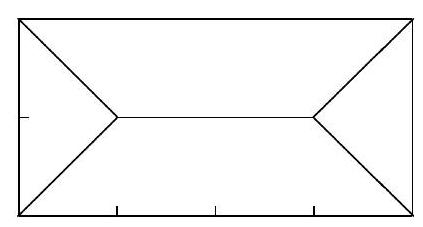
\includegraphics[max width=\textwidth, center]{2024_11_16_fe5b564401bf7db98894g-022}\\
15.4. Pewna firma przeprowadza co kwartał regulacje płac dla swoich pracowników, waloryzujac je zgodnie ze wskaźnikiem inflacji, który jest stały i wynosi $1,5 \%$ kwartalnie, oraz doliczajac stała kwotę podwyżki 16 zł. W styczniu 2001 pan Kowalski otrzymal wynagrodzenie 1600 zł. Jaka pensję otrzyma w kwietniu 2002? Wyznaczyć wzór ogólny na pensję $w_{n}$ pana Kowalskiego w $n$-tym kwartale, przyjmując, że $w_{1}=1600$ jest płaca w pierwszym kwartale 2001. Obliczyć średnią miesięczną płacę pana Kowalskiego w 2002 roku.\\
15.5. Wyznaczyć funkcję odwrotna do $f(x)=x^{3}, x \in R$. Następnie narysować wykres funkcji $h(x)=\sqrt[3]{(|x|-1)}+1$, wyrażając ja za pomocą $f^{-1}$.\\
15.6. Rozwiązać równanie $\frac{\sin 2 x}{\cos 4 x}=1$.\\
15.7. Dany jest trójkąt o wierzchołkach $A(-2,1), \quad B(-1,-6), \quad C(2,5)$. Za pomocą rachunku wektorowego obliczyć cosinus kąta między dwusieczną kąta $A$ i środkową boku $B C$. Sporządzić rysunek.\\
15.8. Zbadać przebieg zmienności i narysować wykres funkcji

$$
f(x)=x+\frac{x}{x-1}+\frac{x}{(x-1)^{2}}+\frac{x}{(x-1)^{3}}+\ldots
$$

\section*{Praca kontrolna nr 2}
16.1. Cena 1 litra paliwa została obniżona o $15 \%$. Po dwóch tygodniach dokonano kolejnej zmiany ceny 1 litra paliwa, podwyższając ją o $15 \%$. O ile procent końcowa cena paliwa różni się od początkowej?\\
16.2. Wyznaczyć i narysować zbiór złożony z punktów $(x, y)$ płaszczyzny spełniających warunek

$$
x^{2}+y^{2}=8|x|+6|y| .
$$

16.3. Wysokość ostrosłupa trójkątnego prawidłowego wynosi $h$, a kąt między wysokościami ścian bocznych poprowadzonymi z wierzchołka ostrosłupa jest równy $2 \alpha$. Obliczyć pole powierzchni bocznej tego ostrostupa. Sporządzić odpowiednie rysunki.\\
16.4. Z arkusza blachy w kształcie równoległoboku o bokach 30 cm i 60 cm i kacie ostrym $60^{\circ}$ należy odciąć dwa przeciwległe trójkątne narożniki tak, aby powstał romb o możliwie największym polu. Określić przez który punkt na dłuższym boku równoległoboku należy przeprowadzić cięcie oraz obliczyć kąt ostry otrzymanego rombu. Wynik zaokraglić do jednej minuty katowej.\\
16.5. Rozwiązać równanie

$$
2^{\log _{\sqrt{2}} x}=(\sqrt{2})^{\log _{x} 2} \text {. }
$$

16.6. Wyznaczyć dziedzinę i zbiór wartości funkcji

$$
f(x)=\frac{4}{\sin x+2 \cos x+3} .
$$

16.7. Znaleźć wszystkie wartości parametru $p$, dla których równanie

$$
p x^{4}-4 x^{2}+p+1=0
$$

ma dwa różne pierwiastki.\\
16.8. Wyznaczyć tangens kata, pod którym styczna do wykresu funkcji

$$
f(x)=\frac{8}{x^{2}+3}
$$

w punkcie $A\left(3, \frac{2}{3}\right)$ przecina ten wykres.

\section*{Praca kontrolna nr 3}
17.1. Dla jakich wartości $\sin x$ liczby $\sin x, \cos x, \sin 2 x$ (w podanym porządku) są kolejnymi wyrazami ciągu geometrycznego? Wyznaczyć czwarty wyraz tego ciagu dla każdego z rozwiązań.\\
17.2. W pewnych zawodach sportowych startuje 16 drużyn. W eliminacjach sa one losowo dzielone na 4 grupy po 4 drużyny w każdej grupie. Obliczyć prawdopodobieństwo tego, że trzy zwycięskie drużyny z poprzednich zawodów znajdą się w trzech różnych grupach.\\
17.3. Nie wykonujac dzielenia, udowodnić, że wielomian

$$
\left(x^{2}+x+1\right)^{3}-x^{6}-x^{3}-1
$$

jest podzielny przez trójmian $(x+1)^{2}$.\\
17.4. Wyznaczyć równanie okręgu o promieniu $r$ stycznego do paraboli $y=x^{2} \mathrm{w}$ dwóch punktach. Dla jakiego $r$ zadanie ma rozwiązanie? Sporzadzić rysunek, przyjmując $r=3 / 2$.\\
17.5. Stosując zasadę indukcji matematycznej, udowodnić prawdziwość wzoru

$$
\binom{2}{2}-\binom{3}{2}+\binom{4}{2}-\binom{5}{2}+\ldots+\binom{2 n}{2}=n^{2}, \quad n \geq 1
$$

17.6. Rozwiązać nierówność

$$
\log _{x}\left(1-6 x^{2}\right) \geq 1
$$

17.7. W trapezie $A B C D$ opisanym na okręgu o środku $S$ dane są ramie $|A D|=c$ oraz $|A S|=d$. Punkt styczności okręgu z podstawa $A B$ dzieli ją w stosunku $1: 2$. Obliczyć pole tego trapezu. Sporządzić rysunek dla $c=5$ i $d=4$.\\
17.8. Wszystkie ściany równoległościanu są rombami o boku a i kącie ostrym $\beta$. Obliczyć objętość tego równoległościanu. Sporządzić rysunek. Obliczenia odpowiednio uzasadnić.

\section*{Praca kontrolna nr 4}
18.1. Obliczyć granicę ciagu o wyrazie ogólnym

$$
a_{n}=\frac{2^{n}+2^{n+1}+\ldots+2^{2 n}}{2^{2}+2^{4}+\ldots+2^{2 n}}
$$

18.2. Wyznaczyć równanie prostej prostopadłej do prostej o równaniu $2 x+3 y+3=0$ i leżącej w równej odległości od dwóch danych punktów $A(-1,1)$ i $B(3,3)$. Sporządzić rysunek.\\
18.3. Tworząca stożka ma długość $l$ i widać ją ze środka kuli wpisanej w ten stożek pod katem $\alpha$. Obliczyć objętość i kąt rozwarcia stożka. Określić dziedzinę kąta $\alpha$.\\
18.4. Bolek kupił jeden długopis i $k$ zeszytów, zapłacił $k$ zł i 50 gr, a Lolek kupił $k$ długopisów i 4 zeszyty, i zapłacił $2,5 k$ zł. Wyznaczyć cenę długopisu i zeszytu w zależności od parametru $k$. Znaleźć wszystkie możliwe wartości tych cen wiedząc, że zeszyt kosztuje nie mniej niż 50 gr, długopis jest droższy od zeszytu, a ceny obydwu artykułów wyrażaja się w pełnych złotych i dziesiątkach groszy.\\
18.5. Rozwiązać nierówność $\operatorname{tg}^{3} x \geq \sin 2 x$.\\
18.6. Żarówki są sprzedawane w opakowaniach po 6 sztuk. Prawdopodobieństwo, że pojedyncza żarówka jest dobra wynosi $\frac{2}{3}$. Jakie jest prawdopodobieństwo tego, że w jednym opakowaniu znajda się co najmniej 4 dobre żarówki. O ile zwiększy się prawdopodobieństwo tego zdarzenia, jeśli jedna, wylosowana z opakowania żarówka, okazała się dobra.\\
18.7. Prosta styczna w punkcie $P$ do okręgu o promieniu 2 i półprosta wychodząca ze środka okręgu mająca z okregiem punkt wspólny $S$ przecinają się w punkcie $A$ pod kątem $60^{\circ}$. Znaleźć promień okręgu stycznego do odcinków $A P, A S$ i łuku $P S$. Sporzadzić rysunek.\\
18.8. W ostrosłupie prawidłowym, którego podstawa jest kwadrat, pole każdej z pięciu ścian wynosi 1 . Ostrosłup ten ścięto płaszczyzną równoległą do podstawy tak, aby uzyskać maksymalny stosunek objętości do pola powierzchni całkowitej. Obliczyć pole powierzchni całkowitej otrzymanego ostrosłupa ściętego. Sporządzić rysunek.

\section*{Praca kontrolna nr 5}
19.1. W czworokacie $A B C D$ dane są wktory $\overrightarrow{A B}=[2,-1], \overrightarrow{B C}=[3,3]$, $\overrightarrow{C D}=[-4,1]$. Punkty $K$ i $M$ sa środkami boków $C D$ oraz $A D$. Za pomoca rachunku wektorowego obliczyć pole trójkąta KMB. Sporzadzić rysunek.\\
19.2. Trzy różne krawędzie oraz przekątna prostopadłościanu tworzą cztery kolejne wyrazy ciagu arytmetycznego. Wyznaczyć sumę długości wszystkich krawędzi tego prostopadłościanu, jeśli przekątna ma długość 7 cm .\\
19.3. Na płaszczyźnie $O x y$ dane sa zbiory $A=\left\{(x, y): y \leq \sqrt{5 x-x^{2}}\right\}$ oraz $B_{s}=\{(x, y): 3 x+4 y=s\}$. Dla jakich wartości parametru $s$ zbiór $A \cap B_{s}$ nie jest pusty? Sporządzić rysunek.\\
19.4. Działka gruntu ma kształt trapezu o bokach $20 \mathrm{~m}, 30 \mathrm{~m}, 40 \mathrm{~m}$ i 60 m . Właściciel działki twierdzi, że powierzchnia jego działki wynosi ponad 11 arów. Czy właściciel ma rację? Jeśli tak, to narysować plan działki w skali 1:1000 i podać jej dokładna powierzchnię.\\
19.5. Dane jest równanie kwadratowe z parametrem $m$

$$
(m+2) x^{2}+4 \sqrt{m} x+(m-3)=0
$$

Dla jakiej wartości parametru $m$ kwadrat różnicy pierwiastków rzeczywistych tego równania jest największy. Podać tẹ największą wartość.\\
19.6. Stosując zasadę indukcji matematycznej, udowodnić, że dla każdego $n \geq 2$ liczba $2^{2^{n}}-6$ jest podzielna przez 10 .\\
19.7. Rozwiązać układ równań

$$
\left\{\begin{array}{l}
\operatorname{tg} x+\operatorname{tg} y=4 \\
\cos (x+y)+\cos (x-y)=\frac{1}{2}
\end{array} \quad \text { dla } x, y \in[-\pi, \pi]\right.
$$

19.8. Równoramienny trójkąt prostokątny $A B C$ zgięto wzdłuż środkowej $C D$ wychodzącej z wierzchołka kata prostego $C$ tak, że obie połowy tego trójkąta utworzyły kat $60^{\circ}$. Obliczyć sinusy wszystkich kątów dwuściennych otrzymanego czworościanu $A B C D$. Rozwiązanie zilustrować odpowiednimi rysunkami, a obliczenia uzasadnić.

\section*{Praca kontrolna nr 6}
20.1. Wyznaczyć wszystkie wartości parametru rzeczywistego $m$, dla których prosta $x=m$ jest osia symetrii wykresu funkcji $p(x)=\left(m^{2}-2 m\right) x^{2}-(2 m-4) x+3$. Sporzadzić rysunek.\\
20.2. Z kuli o promieniu $R$ wycięto ósmą część trzema wzajemnie prostopadłymi płaszczyznami przechodzacymi przez środek kuli. W tak otrzymaną bryłę wpisano inną kulę. Obliczyć stosunek pola powierzchni tej kuli do pola powierzchni bryły.\\
20.3. W trzech pustych urnach $K, L, M$ rozmieszczamy losowo 4 różne kule. Obliczyć prawdopodobieństwo tego, że żadna z urn $K$ i $L$ nie pozostanie pusta.\\
20.4. Dane są punkty $A(2,6), B(-2,6)$ i $C(0,0)$. Wyznaczyć równanie linii zawierającej wszystkie punkty trójkata $A B C$, dla których suma kwadratów ich odległości od trzech boków jest stała i wynosi 9. Sporządzić rysunek.\\
20.5. Narysować dokładny wykres i napisać równania asymptot funkcji

$$
f(x)=\frac{(x+1)^{2}-1}{x|x-1|}
$$

nie badajac jej przebiegu.\\
20.6. Rozwiązać nierówność

$$
|x|^{2 x-1} \leq \frac{1}{x^{2}}
$$

20.7. Styczna do wykresu funkcji $f(x)=\sqrt{3+x}+\sqrt{3-x}$ w punkcie $A\left(x_{0}, f\left(x_{0}\right)\right)$ przecina oś $O x$ w punkcie $P$, a oś $O y$ w punkcie $Q$ tak, że $|O P|=|O Q|$. Wyznaczyć $x_{0}$.\\
20.8. Trójkąt równoboczny o boku a podzielono prosta $l$ na dwie figury, których stosunek pól jest równy $1: 5$. Prosta ta przecina bok $A C$ w punkcie $D$ pod katem $15^{\circ}$, a bok $A B$ w punkcie $E$. Wykazać, że $|A D|+|A E|=a$.

\section*{Praca kontrolna nr 7}
21.1. Sześcian o krawędzi 3 cm ma objętość taką samą jak dwa sześciany, których suma obydwu krawędzi wynosi 4 cm . O ile $\mathrm{cm}^{2}$ pole powierzchni większego sześcianu jest mniejsze od sumy pól powierzchni dwóch mniejszych sześcianów.\\
21.2. Obliczyć tangens kata utworzonego przez przekatne czworokata o wierzchołkach $A(1,1), B(2,0), C(2,4), D(0,6)$. Rozwiązanie zilustrować rysunkiem.\\
21.3. W trójkąt prostokątny wpisano okrag, a w okrag ten wpisano podobny trójkąt prostokątny. Wyznaczyć cosinusy katów ostrych trójkąta, jeśli wiadomo, że stosunek pól obu trójkatów wynosi 9.\\
21.4. Wykazać, że ciagg $a_{n}=\sqrt{n(n+1)}-n$ jest rosnący. Obliczyć jego granicę.\\
21.5. Rozwiązać nierówność

$$
2 \cos ^{2} \frac{x}{4}>1 .
$$

21.6. Rozwiązać równanie

$$
\log _{2}(1-x)+\log _{4}(x+4)=\log _{4}\left(x^{3}-x^{2}-3 x+5\right)+\frac{1}{2}
$$

Nie wyznaczać dziedziny równania w sposób jawny.\\
21.7. W kulę o promieniu $R$ wpisano stożek o największej objętości. Wyznaczyć promień podstawy $r$ i wysokość $h$ tego stożka. Sporządzić rysunek.\\
21.8. Znaleźć równania wszystkich prostych, które są styczne jednocześnie do krzywych

$$
y=-x^{2}, \quad y=x^{2}-8 x+18
$$

Sporządzić rysunek.

\section*{Edycja XXXII}
2002/2003

\section*{Praca kontrolna nr 1}
22.1. Narysować wykres funkcji $y=4+2|x|-x^{2}$. Na podstawie tego wykresu określić liczbę rozwiązań równania $4+2|x|-x^{2}=p$ w zależności od parametru rzeczywistego $p$.\\
22.2. Pompa napełniajaca pusty basen w pierwszej minucie pracy miała wydajność $0,2 \mathrm{~m}^{3} / \mathrm{s}$, a w każdej kolejnej minucie jej wydajność zwiększano o $0,01 \mathrm{~m}^{3} / \mathrm{s}$. Połowa basenu została napetniona po $2 \mathrm{n} \mathrm{mi-}$ nutach, a caty basen po kolejnych $n$ minutach, gdzie $n$ jest liczba naturalną. Wyznaczyć czas napełniania basenu oraz jego pojemność.\\
22.3. Stożek ścięty jest opisany na kuli o promieniu $r=2 \mathrm{~cm}$. Objętość kuli stanowi $25 \%$ objętości stożka. Wyznaczyć średnice podstaw i długość tworzacej tego stożka.\\
22.4. W trójkącie $A B C$ dane sạ promień okręgu opisanego $R$, kąt $\angle A=\alpha$ oraz $|A B|=\frac{8}{5} R$. Obliczyć pole tego trójkąta.\\
22.5. Rozwiązać nierówność

$$
(\sqrt{x})^{\log _{8} x} \geq \sqrt[3]{16 x}
$$

22.6. W czworokacie $A B C D$ odcinki $A B$ i $B D$ są prostopadłe, $|A D|=2|A B|=a$ oraz $\overrightarrow{A C}=\frac{5}{3} \overrightarrow{A B}+\frac{1}{3} \overrightarrow{A D}$. Wyznaczyć cosinus kạta $\angle B C D=\alpha$ oraz obwód czworokąta $A B C D$. Sporządzić rysunek.\\
22.7. Rozwiązać równanie

$$
\frac{1}{\sin x}+\frac{1}{\cos x}=\sqrt{8}
$$

22.8. Wyznaczyć równanie prostej stycznej do wykresu funkcji $y=\frac{1}{x^{2}}$ w punkcie $P\left(x_{0}, y_{0}\right), x_{0}>0$, takim, żeby odcinek tej stycznej zawarty w pierwszej ćwiartce układu współrzędnych był najkrótszy. Rozwiązanie zilustrować odpowiednim wykresem.

\section*{Praca kontrolna nr 2}
23.1. Czy liczby różnych ,„łów", jakie można utworzyć zmieniajac kolejność liter w ,,słowach" TANATAN i AKABARA, sa takie same? Uzasadnić odpowiedź. Przez ,,słowo" rozumiemy tutaj dowolny ciag liter.\\
23.2. Reszta z dzielenia wielomianu $x^{3}+p x^{2}-x+q$ przez trójmian $(x+2)^{2}$ wynosi $(-x+1)$. Wyznaczyć pierwiastki tego wielomianu.\\
23.3. Figura na rysunku składa się z łuków $B C, C A$ okręgów o promie-\\
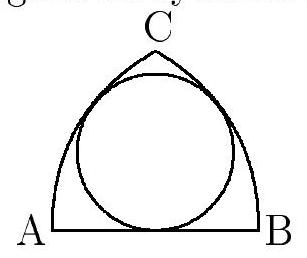
\includegraphics[max width=\textwidth, center]{2024_11_16_fe5b564401bf7db98894g-031(1)}\\
niu $a$ i środkach odpowiednio w punktach $A, B$, oraz z odcinka $A B$ o długości $a$. Obliczyć promień okręgu stycznego do obu łuków oraz do odcinka $A B$.\\
23.4. Podstawa pryzmy przedstawionej na rysunku jest prostokat\\
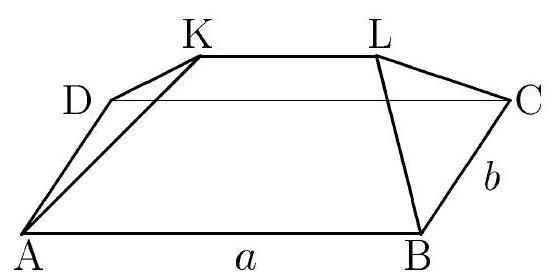
\includegraphics[max width=\textwidth, center]{2024_11_16_fe5b564401bf7db98894g-031}\\
$A B C D$, którego bok $A B$ ma długość $a$, a bok $B C$ długość $b$, gdzie $a>b$. Wszystkie ściany boczne pryzmy sa nachylone pod katem $\alpha$ do płaszczyzny podstawy. Obliczyć objętość tej pryzmy.\\
23.5. Rozwiązać nierówność

$$
\frac{2}{x}<\sqrt{5-x^{2}}
$$

Rozwiązanie zilustrować wykresami funkcji występujacych po obu stronach nierówności. Zaznaczyć na rysunku otrzymany zbiór rozwiązań.\\
23.6. Ciagg $\left(a_{n}\right)$ jest określony rekurencyjnie warunkami $a_{1}=4$, $a_{n+1}=1+2 \sqrt{a_{n}}, n \geq 1$. Stosując zasadę indukcji matematycznej, wykazać, że ciag $\left(a_{n}\right)$ jest rosnący oraz $4 \leq a_{n}<6$ dla $n \geq 1$.\\
23.7. Na krzywej o równaniu $y=\sqrt{x}$ znaleźć punkt leżący najbliżej punktu $P(0,3)$. Sporządzić rysunek.\\
23.8. Wykazać, że dla każdej wartości parametru $\alpha \in \mathbf{R}$ równanie kwadratowe $3 x^{2}+4 x \sin \alpha-\cos 2 \alpha=0$ ma dwa różne pierwiastki rzeczywiste. Wyznaczyć te wartości parametru $\alpha$, dla których oba pierwiastki leżą w przedziale $(0,1)$.

\section*{Praca kontrolna nr 3}
24.1. Suma wyrazów nieskończonego ciągu geometrycznego zmniejszy się o $25 \%$, jeśli wykreślimy z niej składniki o numerach parzystych niepodzielnych przez 4. Obliczyć sumę wszystkich wyrazów tego ciagu, wiedząc, że jego drugi wyraz wynosi 1.\\
24.2. Z kompletu 28 kości do gry w domino wylosowano dwie kości (bez zwracania). Obliczyć prawdopodobieństwo tego, że kości pasuja do siebie, tzn. na jednym z pól obu kości występuje ta sama liczba oczek.\\
24.3. Rozwiązać układ równań

$$
\left\{\begin{array}{l}
x+2 y=3 \\
5 x+m y=m
\end{array}\right.
$$

w zależności od parametru rzeczywistego $m$. Wyznaczyć i narysować zbiór, jaki tworza rozwiązania $(x(m), y(m)$ ) tego układu, gdy $m$ przebiega zbiór liczb rzeczywistych.\\
24.4. W graniastosłupie prawidłowym sześciokątnym krawędź dolnej podstawy $A B$ widać ze środka górnej podstawy $P$ pod katem $\alpha$. Wyznaczyć cosinus kąta utworzonego przez płaszczyznę podstawy i płaszczyznę zawierająca krawędź $A B$ oraz przeciwległạ do niej krawędź $D^{\prime} E^{\prime}$ górnej podstawy. Uzasadnić odpowiednio obliczenia.\\
24.5. Rozwiązać nierówność $-1 \leq \frac{2^{x+1 / 2}}{4^{x}-4} \leq 1$.\\
24.6. Bez użycia tablic wykazać, że $\operatorname{tg} 82^{\circ} 30^{\prime}-\operatorname{tg} 7^{\circ} 30^{\prime}=4+2 \sqrt{3}$.\\
24.7. Napisać równanie prostej $k$ stycznej w punkcie $P(2,3)$ do okręgu $x^{2}+y^{2}-2 x-2 y-3=0$. Następnie wyznaczyć równania wszystkich prostych stycznych do tego okręgu, które tworzą z prostą $k$ kąt $45^{\circ}$.\\
24.8. Dobrać parametry $a>0$ i $b \in R$ tak, aby funkcja

$$
f(x)= \begin{cases}(a+1)+a x-x^{2}, & \text { dla } x \leq a \\ \frac{b}{x^{2}-1}, & \text { dla } x>a\end{cases}
$$

była ciagłła i miała pochodna w punkcie $x=a$. Sporządzić wykres funkcji $f(x)$ oraz stycznej do wykresu w punkcie $P(a, f(a))$ bez szczegółowego badania jej przebiegu.

\section*{Praca kontrolna nr 4}
25.1. Dla jakich wartości parametru rzeczywistego $t$ równanie $x+3=-(t x+1)^{2}$ ma dokładnie jeden pierwiastek.\\
25.2. Czworościan foremny o krawędzi $a$ przecięto płaszczyzną równoległą do dwóch przeciwległych krawędzi. Wyrazić pole otrzymanego przekroju jako funkcję długości odcinka wyznaczonego przez ten przekrój na jednej z pozostałych krawędzi. Uzasadnić postępowanie. Przedstawić znalezioną funkcję na wykresie i podać jej największa wartość.\\
25.3. Zaznaczyć na wykresie zbiór punktów $(x, y)$ płaszczyzny spełniających warunek $\log _{x y}|y| \geq 1$.\\
25.4. Wyznaczyć równanie linii utworzonej przez wszystkie punkty płaszczyzny, których odległość od okręgu $x^{2}+y^{2}=81$ jest o 1 mniejsza niż od punktu $P(8,0)$. Sporządzić rysunek.\\
25.5. Na dziesiątym piętrze pewnego bloku mieszkają Kowalscy i Nowakowie. Kowalscy maja dwóch synów i dwie córki, a Nowakowie jednego syna i dwie córki. Postanowili oni wybrać młodzieżowego przedstawiciela swojego piętra. W tym celu Kowalscy wybrali losowo jedno ze swoich dzieci i Nowakowie jedno ze swoich. Następnie spośród tej dwójki wylosowano jedną osobę. Obliczyć prawdopodobieństwo, że przedstawicielem został chłopiec.\\
25.6. Uzasadnić prawdziwość nierówności $n+\frac{1}{2} \geq \sqrt{n(n+1)}, n \geq 1$. Korzystając z niej oraz z zasady indukcji matematycznej, udowodnić, że

$$
\binom{2 n}{n} \geq \frac{4^{n}}{2 \sqrt{n}}
$$

dla każdej liczby naturalnej $n$.\\
25.7. Zbadać przebieg zmienności i narysować wykres funkcji

$$
f(x)=\sqrt{\frac{3 x-3}{5-x}}
$$

25.8. W trójkącie $A B C$ kạt $A$ ma miarę $\alpha$, kạt $B$ miarę $2 \alpha$, a $|B C|=a$. Oznaczmy kolejno przez $A_{1}$ punkt na boku $A C$ taki, że $B A_{1}$ jest dwusieczna kąta $B ; B_{1}$ punkt na boku $B C$ taki, że $A_{1} B_{1}$ jest dwusieczną katata $A_{1}$, itd. Wyznaczyć długość nieskończonej łamanej $A B A_{1} B_{1} A_{2} \ldots$

\section*{Praca kontrolna nr 5}
26.1. Jakiej długości powinien być pas transmisyjny, aby można go było użyć do połaczenia dwóch kół o promieniach 20 cm i 5 cm , jeśli odległość środków tych kół wynosi 30 cm ?\\
26.2. Umowa określa wynagrodzenie na kwotę 4000 zł. Składka na ubezpieczenie społeczne wynosi $18,7 \%$ tej kwoty, a składka na Kasę Chorych $7,75 \%$ kwoty pozostałej po odliczeniu składki na ubezpieczenie społeczne. W celu obliczenia podatku należy od $80 \%$ wyjściowej kwoty umowy odjąć składkę na ubezpieczenie społeczne i wyznaczyć $19 \%$ pozostałej sumy. Podatek jest różnicą tak otrzymanej liczby i składki na Kasę Chorych. Ile wynosi podatek?.\\
26.3. Przez punkt $P(1,3)$ poprowadzić prosta $l$, tak aby odcinek tej prostej zawarty między prostymi $x-y+3=0$ i $x+2 y-12=0$ dzielił się w punkcie $P$ na połowy. Wyznaczyć równanie ogólne prostej $l$ i obliczyć pole trójkąta, jaki prosta $l$ tworzy z danymi prostymi.\\
26.4. Podstawa czworościanu $A B C D$ jest trójkạt prostokatny $A B C$ o kącie ostrym $\alpha$ i promieniu okręgu wpisanego $r$. Spodek wysokości opuszczonej z wierzchołka $D$ leży w punkcie przecięcia się dwusiecznych trójkąta $A B C$, a ściany boczne wychodzace z wierzchołka kąta prostego podstawy tworzą kat $\beta$. Obliczyć objętość tego ostrosłupa.\\
26.5. Sporzadzić wykres funkcji $f(x)=\log _{4}(2|x|-4)^{2}$. Odczytać z wykresu wszystkie ekstrema lokalne tej funkcji.\\
26.6. Rozwiązać równanie $\cos 2 x+\frac{\operatorname{tg} x}{\sqrt{3}+\operatorname{tg} x}=0$.\\
26.7. Dla jakich wartości parametru $a \in \mathbf{R}$ można określić funkcję $g(x)=f(f(x))$, gdzie $f(x)=\frac{x^{2}}{a x-1}$. Napisać wzór funkcji $g(x)$. Wyznaczyć asymptoty funkcji $g(x)$ dla największej możliwej całkowitej wartości parametru $a$.\\
26.8. Odcinek o końcach $A(0,3), B(2, y), y \in[0,3]$, obraca się wokół osi $O x$. Wyznaczyć pole powierzchni bocznej powstałej bryły jako funkcję $y$ i znaleźć najmniejszą wartość tego pola. Sporządzić rysunek.

\section*{Praca kontrolna nr 6}
27.1. Znaleźć wszystkie wartości parametru rzeczywistego $p$, dla których równanie $\sqrt{x+8 p}=\sqrt{x}+2 p$ ma rozwiązanie.\\
27.2. Obrazem okręgu $K$ w jednokładności o środku $S(0,1)$ i skali $k=-3$ jest okrag $K_{1}$, natomiast obrazem $K_{1}$ w symetrii względem prostej o równaniu $2 x+y+3=0$ jest okrag o tym samym środku co okrag $K$. Wyznaczyć równanie okręgu $K$, jeśli wiadomo, że okręgi $K$ i $K_{1}$ są styczne zewnętrznie.\\
27.3. W trapezie równoramiennym dane są promień okręgu opisanego $r$, kat ostry przy podstawie $\alpha$ oraz suma długości obu podstaw $d$. Obliczyć długość ramienia tego trapezu. Zbadać warunki rozwiązalności zadania. Sporzadzić rysunek dla $\alpha=60^{\circ}, d=\frac{5}{2} r$.\\
27.4. W ostrosłupie prawidłowym czworokątnym kạt płaski ściany bocznej przy wierzchołku wynosi $2 \beta$. Przez wierzchołek $A$ podstawy oraz środek przeciwległej krawędzi bocznej poprowadzono płaszczyznę równoległą do przekątnej podstawy wyznaczająca przekrój płaski ostrosłupa. Obliczyć objętość ostrosłupa, wiedząc, że pole przekroju wynosi $S$.\\
27.5. Obliczyć granicę

$$
\lim _{n \rightarrow \infty} \frac{n-\sqrt[3]{n^{3}+n^{\alpha}}}{\sqrt[5]{n^{3}}}
$$

jeśli $\alpha$ jest najmniejszym dodatnim pierwiastkiem równania $2 \cos \alpha=-\sqrt{3}$.\\
27.6. Rozwiązać nierówność

$$
2^{1+2 \log _{2} \cos x}-\frac{3}{4} \geq 9^{0,5+\log _{3} \sin x}
$$

27.7. Wylosowano, ze zwracaniem, 4 liczby czterocyfrowe (cyfra tysięcy nie może być zerem!). Obliczyć prawdopodobieństwo tego, że co najmniej dwie z tych liczb czytane od strony lewej do prawej lub od strony prawej do lewej będa podzielne przez 4.\\
27.8. Zaznaczyć na rysunku zbiór punktów $(x, y)$ płaszczyzny określony warunkami $|x-3 y|<2$ oraz $y^{3} \leq x$. Obliczyć tangens kata, pod którym przecinaja się linie tworzace brzeg tego zbioru.

\section*{Praca kontrolna nr 7}
28.1. Dwa punkty poruszaja się ruchem jednostajnym po okręgu w tym samym kierunku, przy czym jeden z nich wyprzedza drugi co 44 sekundy. Jeżeli zmienić kierunek ruchu jednego z tych punktów na przeciwny, to będą się one spotykać co 8 sekund. Obliczyć stosunek prędkości tych punktów.\\
28.2. Dla jakich wartości parametru $p$ nierówność

$$
\frac{2 p x^{2}+2 p x+1}{x^{2}+x+2-p^{2}} \geq 2
$$

jest spełniona dla każdej liczby rzeczywistej $x$ ?\\
28.3. W równoległoboku dane są kạt ostry $\alpha$, dłuższa przekatna $d$ oraz różnica boków $r$. Obliczyć pole równoległoboku.\\
28.4. Naczynie w kształcie półkuli o promieniu $R$ ma trzy nóźki w kształcie kulek o promieniu $r, 4 r<R$, przymocowanych do naczynia w ten sposób, że ich środki tworzą trójkąt równoboczny, a naczynie postawione na płaskiej powierzchni dotyka ją w jednym punkcie. Obliczyć wzajemna odległość punktów przymocowania kulek. Sporządzić odpowiednie rysunki.\\
28.5. Za pomocą metod rachunku różniczkowego określić liczbę rozwiązań równania $\quad 2 x^{3}+1=6|x|-6 x^{2}$.\\
28.6. Bez stosowania zasady indukcji matematycznej wykazać, że $\frac{n^{n}-1}{n-1}$ jest nieparzystą liczbą naturalną dla wszystkich $n \geq 2$.\\
28.7. Rozwiązać równanie

$$
\frac{8}{3}\left(\sin ^{2} x+\sin ^{4} x+\ldots\right)=4-2 \cos x+3 \cos ^{2} x-\frac{9}{2} \cos ^{3} x+\ldots
$$

28.8. Rozważmy rodzinę prostych normalnych do paraboli o równaniu $2 y=x^{2}$ (tj. prostopadłych do stycznych w punktach styczności). Znaleźć równanie krzywej utworzonej ze środków odcinków tych normalnych zawartych między osią rzędnych i wyznaczającymi je punktami paraboli. Sporzadzić rysunek.

\section*{Edycja XXXIII}
2003/2004

\section*{Praca kontrolna nr 1}
29.1. Podstawa trójkąta równoramiennego jest odcinek $A B$ o końcach $A(-1,3), B(1,-1)$, a wierzchołek $C$ tego trójkata leży na prostej $l$ o równaniu $3 x-y-14=0$. Obliczyć pole trójkata $A B C$.\\
29.2. Pewna liczba sześciocyfrowa zaczyna się (z lewej strony) cyfrą 3. Jeśli cyfrę tę przestawimy z pierwszej pozycji na ostatnia, to otrzymamy liczbę stanowiącą 25\% liczby pierwotnej. Znaleźć tę liczbę.\\
29.3. W trapezie opisanym na okręgu katy ostre przy podstawie maja miary $\alpha$ i $2 \alpha$, a długość krótszego ramienia wynosi $c$. Obliczyć długość krótszej podstawy tego trapezu. Wynik przedstawić w najprostszej postaci.\\
29.4. Rozwiązać nierówność

$$
\frac{1}{x^{2}-x-2} \leq \frac{1}{|x|}
$$

29.5. Zaznaczyć na płaszczyźnie zbiór wszystkich punktów $(x, y)$ spełniajacych nierówność $\log _{x}\left(1+(y-1)^{3}\right) \leq 1$.\\
29.6. Rozwiązać równanie $\sin ^{2} 3 x-\sin ^{2} 2 x=\sin ^{2} x$.\\
29.7. Wysokość ostrosłupa prawidłowego czworokątnego jest trzy razy dłuższa od promienia kuli wpisanej w ten ostrosłup. Obliczyć cosinus kąta między sasiednimi ścianami bocznymi tego ostrostupa.\\
29.8. Dany jest nieskończony ciag geometryczny

$$
x+1,-x^{2}(x+1), x^{4}(x+1), \ldots
$$

Wyznaczyć najmniejszą i największą wartość funkcji $S(x)$ będącej sumą wszystkich wyrazów tego ciagu.

\section*{Praca kontrolna nr 2}
30.1. Trójkąt prostokątny, obracając się wokół jednej i drugiej przyprostokątnej tworzy bryły o objętościach odpowiednio $V_{1}$ i $V_{2}$. Obliczyć objętość bryły powstałej z obrotu tego trójkata wokół dwusiecznej kąta prostego.\\
30.2. Czy można sumę 42000 złotych podzielić na pewną liczbę nagród, tak aby kwoty tych nagród wyrażały się w pełnych setkach złotych, tworzyły ciag arytmetyczny oraz żeby najwyższa nagroda wynosiła 13000 zł? Jeśli tak, to podać liczbę i wysokości tych nagród.\\
30.3 Dane są okręgi o równaniach $(x-1)^{2}+(y-1)^{2}=1$ oraz $(x-2)^{2}+(y-1)^{2}=16$. Wyznaczyć równania wszystkich okręgów stycznych równocześnie do obu danych okręgów oraz do osi $O y$. Sporządzić rysunek.\\
30.4. W równoległoboku kąt ostry między przekątnymi ma miarę $\beta$, a stosunek długości dłuższej przekątnej do krótszej przekątnej wynosi $k$. Obliczyć tangens kąta ostrego tego równoległoboku.\\
30.5. Rozwiązać równanie $\sqrt{4 x-3}-3=\sqrt{2 x-10}$.\\
30.6. Dobrać liczby całkowite $a, b$, tak aby wielomian $6 x^{3}-7 x^{2}+1$ dzielił się bez reszty przez trójmian kwadratowy $2 x^{2}+a x+b$.\\
30.7. Rozwiązać nierówność $\left|2^{x}-3\right| \leq 2^{1-x}$. Sporządzić wykresy funkcji występujących po obu stronach tej nierówności oraz zaznaczyć na rysunku zbiór rozwiązań.\\
30.8. Wyznaczyć przedziały monotoniczności funkcji

$$
f(x)=\sin ^{2} x+\frac{\sqrt{3}}{2} x, \quad x \in[-\pi, \pi] .
$$

\section*{Praca kontrolna nr 3}
31.1. Z talii 24 kart do gry wylosowano 7 kart. Jakie jest prawdopodobieństwo otrzymania dokładnie czterech kart w jednym z czterech kolorów, w tym asa, króla i damę.\\
31.2. Pewien ostrosłup podzielono na trzy części dwiema płaszczyznami równoległymi do jego podstawy. Pierwsza płaszczyzna leży w odległości $d_{1}=2 \mathrm{~cm}$, a druga w odległości $d_{2}=3 \mathrm{~cm}$ od podstawy. Pola przekrojów ostrostupa tymi płaszczyznami równe są odpowiednio $S_{1}=25 \mathrm{~cm}^{2}$ oraz $S_{2}=16 \mathrm{~cm}^{2}$. Obliczyć objętość tego ostrostupa oraz objętość najmniejszej części.\\
31.3. Rozwiązać układ równań $\left\{\begin{array}{l}x^{2}+y^{2}=24 \\ \frac{2 \log x+\log y^{2}}{\log (x+y)}=2 .\end{array}\right.$\\
31.4. W trójkącie równoramiennym $A B C$ odległość środka okręgu wpisanego od wierzchołka $C$ wynosi $d$, a podstawę $A B$ widać ze środka okręgu wpisanego pod katem $\alpha$. Obliczyć pole tego trójkata.\\
31.5. Stosując zasadę indukcji matematycznej, udowodnić prawdziwość dla $n \geq 1$ wzoru

$$
\cos x+\cos 3 x+\ldots+\cos (2 n-1) x=\frac{\sin 2 n x}{2 \sin x}, \quad \sin x \neq 0
$$

31.6. Wyznaczyć granicę ciągu o wyrazie ogólnym

$$
a_{n}=\frac{\sqrt[6]{4 n}}{\sqrt{n}-\sqrt{n+\sqrt[3]{4 n^{2}}}}, n \geq 1
$$

31.7. Dany jest wierzchołek $A(6,1)$ kwadratu. Wyznaczyć pozostałe wierzchołki tego kwadratu, gdy wierzchołki sạsiadujace z $A$ leżą jeden na prostej $l: x-2 y+1=0$, a drugi na prostej $k: x+3 y-4=0$. Sporzadzić rysunek.\\
31.8. Zbadać przebieg zmienności i narysować wykres funkcji

$$
f(x)=\frac{x+1}{\sqrt{x}}
$$

\section*{Praca kontrolna nr 4}
32.1. Statek z Wrocławia do Szczecina płynie 3 dni, a ze Szczecina do Wrocławia 5 dni. Jak długo z Wrocławia do Szczecina płynie woda?\\
32.2. Dla jakich wartości rzeczywistych $x$ liczby $1+\log _{2} 3, \log _{x} 36$, $\frac{4}{3} \log _{8} 6$ są trzema kolejnymi wyrazami ciagu geometrycznego.\\
32.3. Wanna o pojemności 200 l mająca ksztalt połowy walca (rozciętego wzdłuż osi) leży poziomo na ziemi i zawiera pewną ilość wody. Do wanny włożono belkę (cięższą od wody) w kształcie walca o średnicy cztery razy mniejszej niż średnica wanny i długości równej połowie długości wanny. Okazało się, że lustro wody styka się z powierzchnia belki zanurzonej w wodzie. Podać, z dokładnością do $0,1 \mathrm{l}$, ile wody znajduje się w wannie?\\
32.4. Wyznaczyć wszystkie wartości parametru $m$, dla których obydwa pierwiastki trójmianu kwadratowego $v(x)=x^{2}+m x-m^{2}$ leżą między pierwiastkami trójmianu $w(x)=x^{2}-(m-1) x-m$.\\
32.5. Urna A zawiera trzy kule białe i dwie czarne, a urna B dwie kule białe i trzy czarne. Wylosowano cztery razy jedną kulę (ze zwracaniem) z urny A oraz jedną kulę z urny B. Obliczyć prawdopodobieństwo tego, że wśród pięciu wylosowanych kul są co najmniej dwie kule biate.\\
32.6. Rozwiązać równanie $2 \sin 2 x+2 \cos 2 x+\operatorname{tg} x=3$.\\
32.7. Dana jest funkcja $f(x)=x^{4}-2 x^{2}$. Wyznaczyć wszystkie proste styczne do wykresu tej funkcji zawierajace punkt $P(1,-1)$. Ile punktów wspólnych z wykresem tej funkcji maja wyznaczone styczne? Rozwiązanie zilustrować rysunkiem.\\
32.8. Podstawa ostrosłupa $A B C S$ jest trójkąt równoramienny, którego kạt przy wierzchołku $C$ ma miarę $\alpha$, a ramię $B C$ ma długość $b$. Spodek wysokości ostrostupa leży w środku wysokości $C D$ podstawy, a kąt płaski ściany bocznej $A B S$ przy wierzchołku ma miarę $\alpha$. Obliczyć promień kuli opisanej na tym ostrosłupie oraz cosinusy kątów nachylenia ścian bocznych do podstawy.

\section*{Praca kontrolna nr 5}
33.1. Piąty wyraz rozwinięcia dwumianu $(a+b)^{18}$, gdzie $a, b>0$, jest o $180 \%$ większy od wyrazu trzeciego. O ile procent wyraz ósmy tego rozwinięcia jest mniejszy bądź większy od wyrazu czwartego?\\
33.2. Wyznaczyć równanie linii utworzonej przez wszystkie punkty płaszczyzny, dla których stosunek kwadratu odległości od prostej $k: x-2 y+3=0$ do kwadratu odległości od prostej $l: 3 x+y+2=0$ wynosi 2 . Sporządzić rysunek.\\
33.3. Obwód trójkąta $A B C$ wynosi 15 cm , a dwusieczna kąta $A$ dzieli bok przeciwległy na odcinki długości 3 cm oraz 2 cm . Obliczyć pole koła wpisanego w ten trójkąt.\\
33.4. Czastka startuje z początku układu współrzędnych i porusza się ze stała prędkościa po nieskończonej łamanej jak na rysunku, której długości kolejnych odcinków tworzą ciąg geometryczny malejacy. Po pewnym czasie czastka zatrzymała się w punkcie $P(10,3)$. Jaką droge przebyła cząstka?\\
33.5. Stosując zasadę indukcji matematycznej, udowodnić, że dla wszystkich $n \geq 1$ wielomian $x^{3 n+1}+x^{3 n-1}+1$ dzieli się bez reszty przez wielomian $x^{2}+x+1$.\\
33.6. Narysować wykres funkcji $f(x)=\frac{|x-2|}{x-|x|+2}$ bez badania jej przebiegu. Podać równania asymptot i ekstrema lokalne tej funkcji.\\
33.7. Rozwiazać nierówność

$$
|\cos x|^{1+\sqrt{2} \sin x+\sqrt{2} \cos x} \leq 1, \quad x \in[-\pi, \pi] .
$$

33.8. W stożek wpisano graniastosłup trójkątny prawidłowy o wszystkich krawędziach tej samej długości, tak że dolna podstawa leży na podstawie stożka. Przy jakim kącie rozwarcia stożka stosunek objętości graniastosłupa do objętości stożka jest największy?

\section*{Praca kontrolna nr 6}
34.1. W koło o polu $\frac{5}{4} \pi$ wpisano trójkat prostokątny o polu 1. Obliczyć obwód tego trójkąta.\\
34.2. Sprowadzić do najprostszej postaci wyrażenie

$$
2\left(\sin ^{6} \alpha+\cos ^{6} \alpha\right)-7\left(\sin ^{4} \alpha+\cos ^{4} \alpha\right)+\cos 4 \alpha
$$

34.3. Wyznaczyć trójmian kwadratowy, którego wykresem jest parabola styczna do prostej $y=x+2$, przechodzaca przez punkt $P(-2,-2)$ oraz symetryczna względem prostej $x=1$. Sporządzić rysunek.\\
34.4. W trapezie $A B C D$, w którym $A B \| C D$, dane są $\overrightarrow{A C}=[4,7]$ oraz $\overrightarrow{B D}=[-6,2]$. Za pomocą rachunku wektorowego wyznaczyć wektory $\overrightarrow{A B}$ i $\overrightarrow{C D}$, jeśli wiadomo, że $\overrightarrow{A D} \perp \overrightarrow{B D}$.\\
34.5. Jaś ma w portmonetce 3 monety jednozłotowe, 2 monety dwuzłotowe i jedna pięciozłotowa. Kupując zeszyt w cenie 4 zł, wyciaga losowo z portmonetki po jednej monecie tak długo, aż uzbiera się suma wystarczająca na kupno zeszytu. Obliczyć prawdopodobieństwo, że Jaś wyciaggnie co najmniej trzy monety. Podać odpowiednie uzasadnienie (nie jest nim tzw. drzewko).\\
34.6. Narysować na płaszczyźnie zbiór punktów określony następująco

$$
\mathcal{F}=\left\{(x, y): \sqrt{4 x-x^{2}} \leq y \leq 4-\sqrt{1-2 x+x^{2}}\right\}
$$

W jakiej odległości od brzegu figury $\mathcal{F}$ znajduje się punkt $P\left(\frac{3}{2}, \frac{5}{2}\right)$ ?\\
34.7. Dana jest funkcja $f(x)=\log _{2}\left(1-x^{2}\right)-\log _{2}\left(x^{2}-x\right)$. Bez stosowania metod rachunku różniczkowego wykazać, że $f$ jest rosnąca w swojej dziedzinie oraz, że $g(x)=f\left(x-\frac{1}{2}\right)$ jest nieparzysta. Wyznaczyć funkcję odwrotną $f^{-1}$, jej dziedzinę i zbiór wartości.\\
34.8. Pole powierzchni bocznej ostrosłupa prawidłowego czworokatnego wynosi $c^{2}$, a kat nachylenia ściany bocznej do podstawy ma miarę $\alpha$. Ostrosłup przecięto na dwie części płaszczyzna przechodzạca przez jeden z wierzchołków podstawy i prostopadła do przeciwległej krawędzi bocznej. Obliczyć objętość części zawierającej wierzchołek ostrosłupa. Podać warunek rozwiązalności zadania.

\section*{Praca kontrolna nr 7}
35.1. Dwa pierwsze wyrazy nieskończonego ciagu geometrycznego sa pierwiastkami równania $4 x^{2}-4 p x-3 p^{2}=0$, gdzie $p$ jest nieznana liczbą. Wyznaczyć ten ciag, jeśli suma wszystkich jego wyrazów wynosi 3.\\
35.2. Wiedzạc, że $\cos \varphi=\sqrt{\frac{2}{3}}$ oraz $\varphi \in\left(\frac{3}{2} \pi, 2 \pi\right)$, obliczyć cosinus kąta pomiędzy prostymi $y=\left(\sin \frac{\varphi}{2}\right) x, y=\left(\cos \frac{\varphi}{2}\right) x$.\\
35.3. Kostka sześcienna ma krawędź $2 a$. Aby zmieścić ją w pojemniku w kształcie kuli o średnicy $3 a$, ze wszystkich narożników odcięto w minimalny sposób jednakowe ostrosłupy prawidłowe trójkątne. Obliczyć długość krawędzi bocznych odciętych czworościanów?\\
35.4. Udowodnić prawdziwość nierówności

$$
1+\frac{x}{2} \geq \sqrt{1+x} \geq 1+\frac{x}{2}-\frac{x^{2}}{2} \text { dla } x \in[-1,1]
$$

Zilustrować ja na odpowiednim wykresie.\\
35.5. Rozwiązać równanie

$$
\frac{\cos 5 x}{\sin 2 x}=-\sin 3 x
$$

35.6. Dany jest okrag $\mathcal{K}: x^{2}-4 x+y^{2}+6 y=0$. Znaleźć równanie okręgu symetrycznego do $\mathcal{K}$ względem stycznej do $\mathcal{K}$ poprowadzonej z punktu $P(3,5)$ i mającej dodatni współczynnik kierunkowy.\\
35.7. W okrag o promieniu $r$ wpisano trapez o przekatnej $d, \quad d \geq r \sqrt{3}$, i największym obwodzie. Obliczyć pole tego trapezu.\\
35.8. Metodą analityczną określić dla jakich wartości parametru $m$ układ równań

$$
\left\{\begin{array}{l}
m x-y+2=0 \\
x-2|y|+2=0
\end{array}\right.
$$

ma dokładnie jedno rozwiązanie. Wyznaczyć to rozwiązanie w zależności od $m$. Sporządzić rysunek.

\section*{Indeks tematyczny}
\section*{1. Liczby rzeczywiste}
\begin{itemize}
  \item Obliczenia procentowe: 1.1, 9.1, 16.1, 26.2, 33.1.
  \item Zasada indukcji matematycznej: 2.1, 3.3, 10.1, 11.5, 17.5, 19.6, 23.6, 25.6, 31.5, 33.5.
  \item Inne: 8.2, 28.6, 33.1.
\end{itemize}

\section*{2. Funkcja liniowa}
\begin{itemize}
  \item Układy równań liniowych z parametrem: 7.5, 12.7, 18.4, 24.3, 35.8.
  \item Wartość bezwzględna: 2.5, 5.1, 13.7, 27.8, 35.8.
  \item Inne: 15.1, 28.1, 29.2, 32.1.
\end{itemize}

\section*{3. Funkcja kwadratowa}
\begin{itemize}
  \item Równania kwadratowe z parametrem: 2.4, 4.7, 5.7, 9.3, 11.7, 13.3, 16.7, 19.5, 20.1, 23.8, 25.1, 28.2, 32.4.
  \item Układy równań drugiego stopnia: 2.6, 10.7, 21.1, 31.3.
  \item Inne: 2.2, 3.1 (10.3), 8.3, 21.8, 22.1, 34.3, 35.1, 35.4.
\end{itemize}

\section*{4. Wielomiany}
\begin{itemize}
  \item 2.1, 12.2, 17.3, 21.1, 23.2, 28.5, 30.6, 33.5.
\end{itemize}

\section*{5. Funkcje wymierne i niewymierne}
\begin{itemize}
  \item Wykresy funkcji: 12.1, 13.7, 15.5, 19.3, 20.5, 26.7, 33.6.
  \item Równania i nierówności: 1.6, 5.4, 9.5, 11.8, 15.2, 23.5, 27.1, 29.4, 30.5 .
\end{itemize}

\section*{6. Funkcje potegowe, wykładnicze i logarytmiczne}
\begin{itemize}
  \item Wykresy funkcji: 1.5, 13.3, 26.5.
  \item Przekształcanie wyrażeń: 14.6, 27.5, 31.6, 32.2.
  \item Równania: 1.2, 6.1, 9.3, 16.5, 21.6, 31.3.
  \item Nierówności: $2.3,4.5,7.1,8.4,10.5,11.7,17.6,20.6,22.5,24.5$, 25.3, 27.6, 29.5, 30.7, 33.7.
\end{itemize}

\section*{7. Funkcje trygonometryczne}
\begin{itemize}
  \item Tożsamości, przekształcanie wyrażeń: 4.3, 5.2, 6.3, 13.1, 14.4, 16.6, 17.1, 24.6, 31.5, 34.2, 35.2 .
  \item Równania: 1.4, 2.8, 8.7, 10.8, 15.6, 19.7, 22.7, 23.8, 26.6, 27.5, 28.7, 29.6, 32.6, 35.5.
  \item Nierówności: 3.8, 7.6, 10.8, 11.4, 18.5, 21.5, 23.8, 27.6, 33.7.
\end{itemize}

\section*{8. Własności funkcji}
\begin{itemize}
  \item 3.1 (10.3), 15.5, 16.6, 26.7, 34.7.
\end{itemize}

\section*{9. Ciagi liczbowe}
\begin{itemize}
  \item Ciag arytmetyczny: 4.1, 13.5, 19.2, 22.2, 30.2.
  \item Ciag geometryczny: 6.4, 15.4, 17.1, 18.1, 32.2.
  \item Ciag geometryczny nieskończony: 1.2, 2.8, 8.1, 11.4, 14.2, 15.8, 24.1, 25.8, 28.7, 29.8, 33.4, 35.1.
  \item Granica ciagu: 14.6, 18.1, 21.4, 27.5, 31.6.
  \item Własności ciagu: 21.4, 23.6.
\end{itemize}

\section*{10. Granica i ciagłość funkcji. Pochodna, styczna}
$\bullet 1.8,4.3,9.8,16.8,20.7,21.8,22.8,23.7,24.8,27.8,32.7$.

\section*{11. Zastosowania pochodnej}
\begin{itemize}
  \item Badanie przebiegu funkcji: 3.6, 4.7, 9.7, 13.8, 15.8, 25.7, 31.8.
  \item Ekstrema lokalne: 8.3, 11.3, 26.5, 28.5, 33.6.
  \item Wartość najmniejsza i największa funkcji w zbiorze: 2.2, 3.1 (10.3), 3.5, 6.7, 10.6, 12.8 (26.8), 18.8, 19.5, 21.7, 22.8, 25.2, 29.8, 33.8, 35.7.
  \item Inne: 5.7, 24.8, 30.8.
\end{itemize}

\section*{12. Geometria analityczna}
\begin{itemize}
  \item Rachunek wektorowy, iloczyn skalarny: 1.3, 5.8 (15.7), 8.6, 13.2, 14.3, 19.1, 21.2, 22.6, 23.7, 29.1, 31.7, 34.4.
  \item Prosta: 3.2, 14.3, 18.2, 26.3, 35.2.
  \item Okrag: 2.7, 6.2, 10.6, 12.4, 16.2, 24.7, 27.2, 30.3, 35.6.
  \item Zbiory punktów o danej własności (miejsca geometryczne punktów): 4.6, 5.3, 9.2, 11.6, 20.4, 25.4, 28.8, 33.2.
  \item Geometryczna interpretacja układów równań i nierówności: 2.6, 4.5, 5.1, 10.7, 13.7, 19.3, 23.5, 25.3, 27.8, 29.5, 34.6.
  \item Inne: 7.2, 14.5, 17.4, 21.8, 34.3.
\end{itemize}

\section*{13. Planimetria}
\begin{itemize}
  \item Trójkąt: 3.5, 6.8, 8.8, 9.6, 11.1, 13.6, 20.8, 21.3, 22.4, 23.3, 25.8, $31.4,33.3,34.1$.
  \item Trapez: 3.7, 7.4, 12.6, 17.7, 19.4, 27.3, 29.3, 35.7.
  \item Inne figury: 4.4, 14.2, 16.4, 18.7, 23.3, 26.1, 28.3, 30.4.
\end{itemize}

\section*{14. Stereometria}
\begin{itemize}
  \item Graniastosłupy: 6.4, 11.2, 19.2, 21.1, 24.4, 35.3.
  \item Ostrosłupy: 1.7, 3.4, 4.8, 7.7 (31.2), 8.5, 9.4, 12.5, 14.8, 16.3, $18.8,19.8,25.2,26.4,27.4,29.7,32.8,34.8$.\\
$\bullet$ Bryły obrotowe: 5.6, 6.6, 10.2 (18.3), 12.8 (26.8), 20.2, 21.7, 22.3, 28.4, 30.1, 32.3, 33.8.
  \item Inne bryły: 15.3, 17.8, 23.4.
\end{itemize}

\section*{15. Rachunek prawdopodobieństwa i kombinatoryka}
\begin{itemize}
  \item Prawdopodobieństwo klasyczne: 4.2, 7.8 (14.7), 10.4, 17.2, 20.3, 24.2, 31.1.
  \item Wzór na prawdopodobieństwo całkowite: 6.5, 12.3, 25.5, 34.5.
  \item Niezależność i schemat Bernoulliego: 5.5, 13.4, 18.6, 27.7, 32.5.
  \item Kombinatoryka: 7.3, 14.1, 23.1.
\end{itemize}

Odpowiedzi\\
do zadań\\
1.1. Masa stopu $2,3 \mathrm{~kg}$, próba stopu 0,690 .\\
1.2. $\log _{3} 2$.\\
1.3. $C\left(\frac{30}{11}, \frac{10}{11}\right)$.\\
1.4. $\frac{\pi}{14}+k \frac{2 \pi}{7}, k \in \mathbf{Z}$.\\
1.5. Rysunek 1.\\
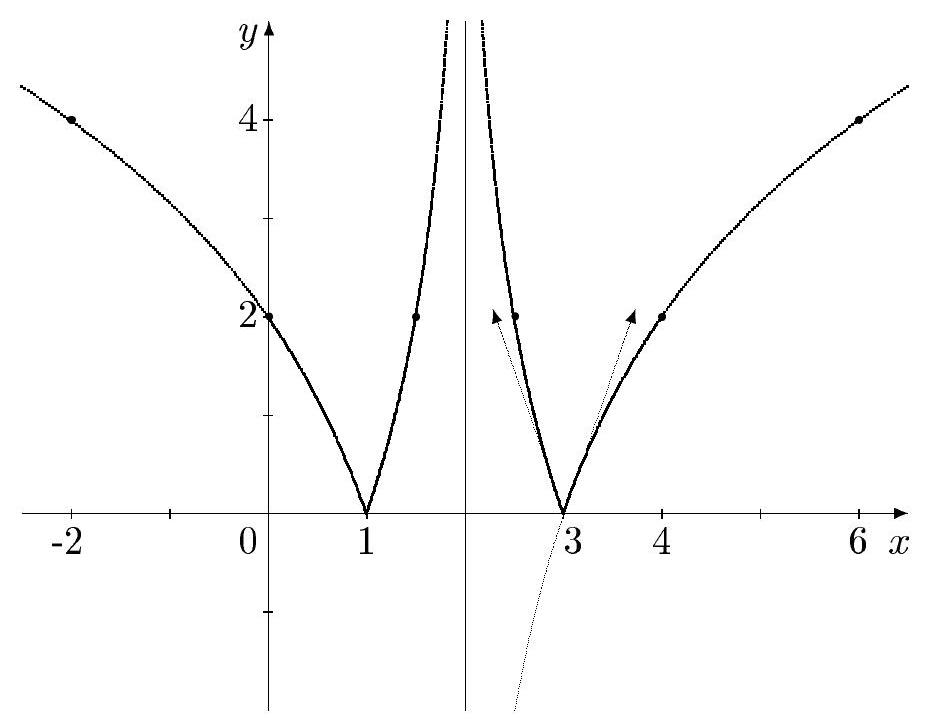
\includegraphics[max width=\textwidth, center]{2024_11_16_fe5b564401bf7db98894g-052}

Rys. 1\\
1.6. $(-\infty,-6) \cup[-2,0) \cup(0,3]$.\\
1.7. $-\frac{3}{5}$.\\
1.8. Sa dwie takie styczne i mają równania $y=-\frac{1}{2} x+2$ oraz $y=-\frac{1}{2} x-2$.\\
2.2. Podstawa prostokąta $a=\frac{2}{5} \sqrt{10} \mathrm{~cm}$, wysokość $b=\frac{4}{5} \sqrt{10} \mathrm{~cm}$, przekatna $p=2 \sqrt{2} \mathrm{~cm}$.\\
2.3. $(1, \sqrt[3]{9}) \cup(\sqrt[3]{9}, \infty)$.\\
2.4. $4-2 \sqrt{2}<p<4+2 \sqrt{2}$.\\
2.5. Dla $m<0$ brak rozwiązań,\\
dla $m=0$ lub $m>1$ sa dwa rozwiązania,\\
dla $m=1$ sa trzy rozwiązania,\\
dla $0<m<1$ są cztery rozwiązania.\\
2.6. Układ ma trzy rozwiązania:

$$
\left\{\begin{array} { l } 
{ x _ { 1 } = - 7 } \\
{ y _ { 1 } = - 1 , }
\end{array} \left\{\begin{array} { l } 
{ x _ { 2 } = 1 } \\
{ y _ { 2 } = 7 , }
\end{array} \left\{\begin{array}{l}
x_{3}=5 \\
y_{3}=-5
\end{array}\right.\right.\right.
$$

2.7. $S=\frac{1225}{12}$.\\
2.8. $\frac{\pi}{8}, \frac{7 \pi}{8}, \frac{9 \pi}{8}, \frac{15 \pi}{8}$.\\
3.1. Dziedziną jest przedział $[0,4]$, a zbiorem wartości przedział $\left[0, \frac{3}{2}\right]$.\\
3.2. Prosta $A B$ ma równanie $y=3$, a prosta $A D$ równanie $4 x-3 y=15$.\\
3.4. $\frac{8}{3} \sqrt{3} \mathrm{~cm}^{3}$.\\
3.5. Trójkat równoboczny o boku $R \sqrt{3}$ i polu $\frac{3 \sqrt{3}}{4} R^{2}$.\\
3.6. $D=\left(-\infty, \frac{5}{2}\right]$; miejsca zerowe $0, \frac{5}{2}$; minimum lokalne 0 dla $x=0$; maksimum lokalne 2 dla $x=2$; funkcja rosnaca w $(0,2)$; malejaca w $(-\infty, 0)$ oraz w $\left(2, \frac{5}{2}\right)$; wypukła w $\left(-\infty, 2-\frac{\sqrt{6}}{3}\right)$; wklęsła w $\left(2-\frac{\sqrt{6}}{3}, \frac{5}{2}\right)$; punkt przegięcia $P\left(2-\frac{\sqrt{6}}{3}, \sqrt{\frac{62 \sqrt{6}-117}{27}}\right)$; prosta $x=\frac{5}{2}$ jest styczna do wykresu funkcji w punkcie $\left(\frac{5}{2}, 0\right)$. Wykres funkcji przedstawiono na rysunku 2.\\
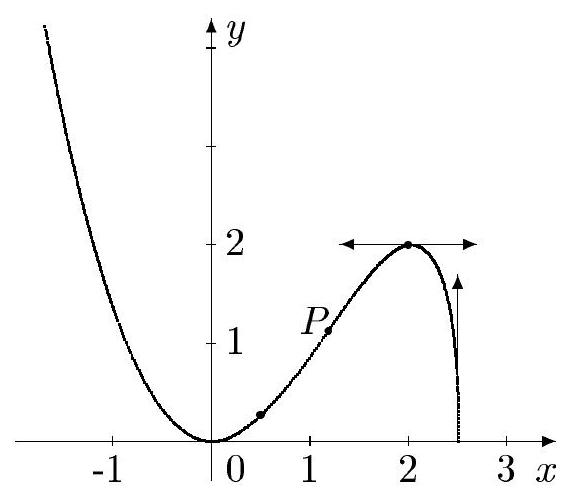
\includegraphics[max width=\textwidth, center]{2024_11_16_fe5b564401bf7db98894g-054}

Rys. 2\\
3.7. $S=\frac{d^{2}-2 d r \cos \alpha+r^{2} \cos 2 \alpha}{2(d-r \cos \alpha)} r \sin \alpha ; \quad R=\frac{d^{2}-2 d r \cos \alpha+r^{2}}{4(d-r \cos \alpha) \sin \alpha}$;\\
rozwiązanie istnieje, gdy $d \geq r(1+2 \cos \alpha)$. Wynik liczbowy $S=\frac{13}{12} \sqrt{3} \mathrm{~cm}^{2}$, $R=\frac{7}{3} \mathrm{~cm}$.\\
3.8. $\left[0, \frac{\pi}{12}\right] \cup\left[\frac{7 \pi}{12}, \frac{13 \pi}{12}\right] \cup\left[\frac{19 \pi}{12}, \frac{25 \pi}{12}\right] \cup\left[\frac{31 \pi}{12}, 3 \pi\right]$.\\
4.1. 109.\\
4.2. $\frac{7}{9}$.\\
4.3. Pochodna nie istnieje.\\
4.5. $\left\{\begin{array}{l}x \leq 1 \\ 1<y \leq 3-x\end{array}\right.$ lub $\left\{\begin{array}{l}0<y<1 \\ 1 \leq x \leq 3-y .\end{array}\right.$\\
4.6. Elipsa o równaniu $\frac{(x+4)^{2}}{36}+\frac{y^{2}}{20}=1$, środku $M(-4,0)$ i półosiach $a=6, b=2 \sqrt{5}$.\\
4.7. $y=f(m)=\frac{4}{m}-\frac{4}{m^{2}} . \quad D=(-\infty, 0) \cup(0,5]$; miejsce zerowe 1 ; asymptota pionowa obustronna $m=0$; asymptota pozioma lewostronna $y=0$; maksimum lokalne 1 dla $m=2$; funkcja rosnąca w $(0,2)$; malejąca w $(-\infty, 0)$ oraz w $(2,5)$; wypukła w $(3,5)$; wklęsła w $(-\infty, 0)$ oraz w $(0,3)$; punkt przegięcia $P\left(3, \frac{8}{9}\right)$. Wykres przedstawiono na rysunku 3.\\
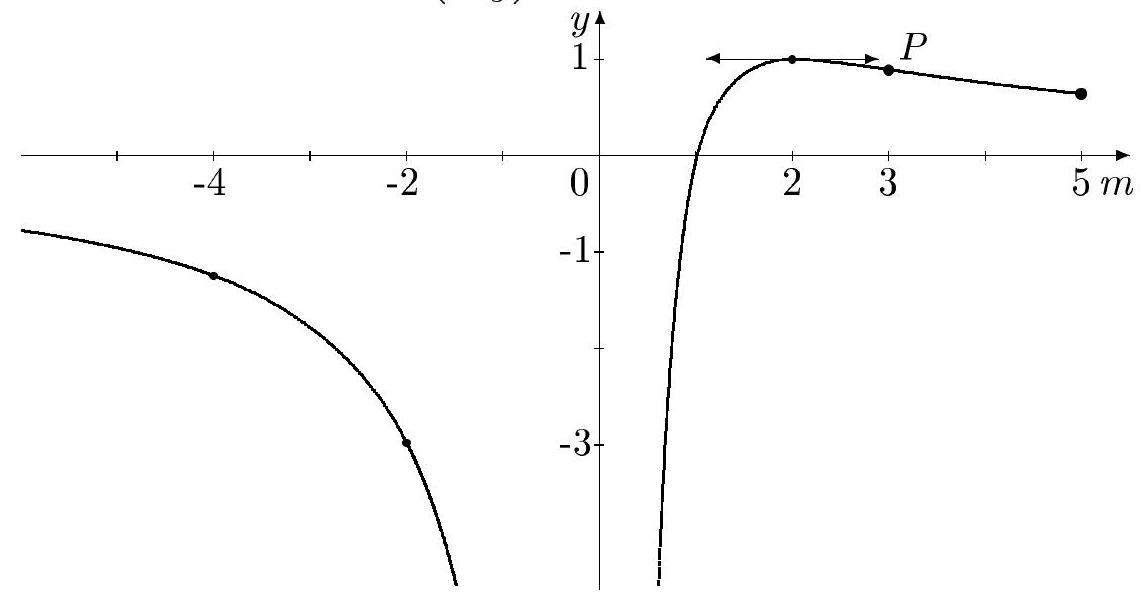
\includegraphics[max width=\textwidth, center]{2024_11_16_fe5b564401bf7db98894g-055(1)}

Rys. 3\\
4.8. $S=\frac{\pi}{16} a^{2} \frac{27-32 \cos ^{2} \alpha}{\cos ^{2} \alpha\left(3-4 \cos ^{2} \alpha\right)}, \alpha \in\left(\frac{\pi}{6}, \frac{\pi}{2}\right)$.\\
5.1. Zbiór $A$ przedstawiono na rysunku 4. Punkt $Q\left(\frac{3}{2}, \frac{5}{2}\right)$ leży najbliżej punktu $P$.\\
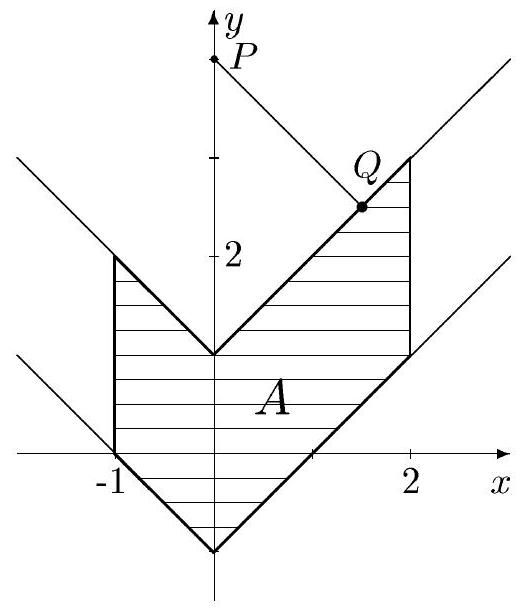
\includegraphics[max width=\textwidth, center]{2024_11_16_fe5b564401bf7db98894g-055}

Rys. 4\\
5.2. $\frac{7}{16} \sqrt{5}$ lub $-\frac{7}{16} \sqrt{5}$.\\
5.3. Szukana krzywą stanowią dwie gatęzie paraboli $y=\frac{1}{2} x^{2}-1$ dla $x \geq 2$ oraz dla $x \leq 2$.\\
5.4. 11.\\
5.5. Pierwszy.\\
5.6. $2 r+4 \sqrt{2 R r-R^{2}}$.\\
5.7. Dla $m \in[2 \sqrt{3}, \infty)$.\\
5.8. $\frac{9}{85} \sqrt{85}$.\\
6.1. $\frac{1}{4}(-3+3 \sqrt{3})$.\\
6.2. $\frac{13}{3}$.\\
6.4. $8+(1+\sqrt{33})^{3 / 2}$.\\
6.5. $\frac{3}{10}$.\\
6.6. $\frac{\pi}{12} d^{3} \operatorname{tg}^{2} \alpha\left(8 \cos ^{4} \alpha-1\right)$.\\
6.7. Wartość najmniejsza 31, a największa $24 \sqrt{2}$.\\
6.8. Stosunek wynosi $1+k$, a dziedzina $k$ jest przedziat $(0, \sqrt{2}-1]$.\\
7.1. $(0,1)$.\\
7.2. Elipsa o równaniu $\frac{(x+1)^{2}}{4}+\frac{(y-3)^{2}}{1}=1$, środku $S(-1,3)$ i półosiach $a=2, \quad b=1$. Pole figury wynosi $2 \pi$.\\
7.3. 330.\\
7.4. $\frac{\pi}{4}(\sqrt{8}-\sqrt{6})$.\\
7.5. Dla $m$ różnych od 3 i 4 jedno rozwiazanie $x=\frac{9}{m-4}, y=\frac{m+2}{m-4}$. Dla $m=4$ układ sprzeczny. Dla $m=3$ nieskończenie wiele rozwiązań spełniajacych warunek $x-2 y=1$, gdzie $x$ dowolne rzeczywiste. Sa dwa rozwiązania spetniajace warunek $x=y$ : dla $m=7(x=y=3)$ oraz dla $m=3(x=y=-1)$.\\
7.6. $\left(-\frac{\pi}{3}, 0\right) \cup\left(\frac{\pi}{3}, \frac{\pi}{2}\right]$.\\
7.7. Objętość ostrosłupa wynosi $\frac{343}{3} \mathrm{~cm}^{3}$, a objętość najmniejszej części $\frac{61}{3} \mathrm{~cm}^{3}$.\\
7.8. a) $\frac{1}{20}$; b) $\frac{7}{20}$.\\
8.1. $q=\frac{1}{30}, \quad a_{1}=1972$.\\
8.2. Są dwa takie składniki 26730 oraz 1320 .\\
8.3. Wykres funkcji przedstawiono na rysunku 5.\\
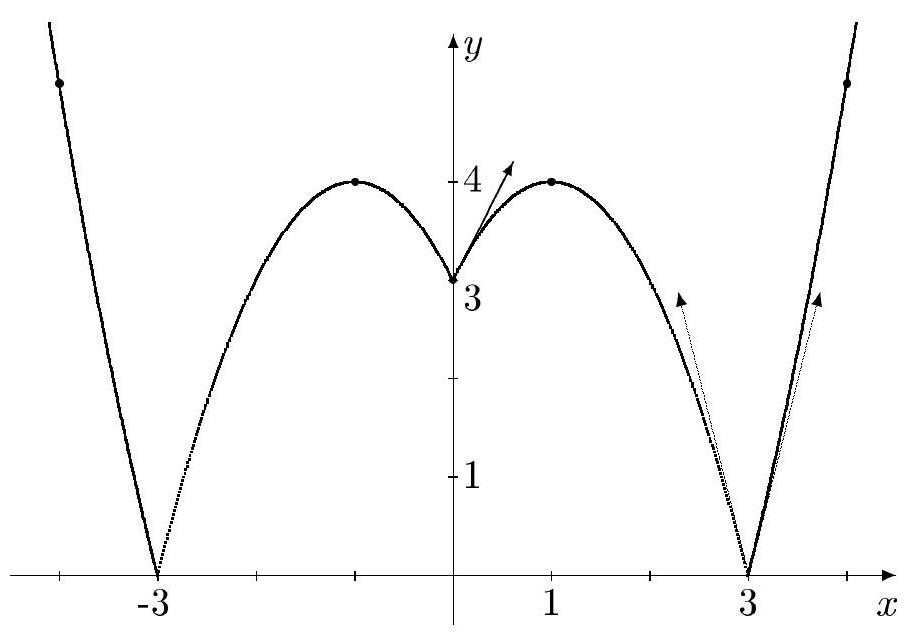
\includegraphics[max width=\textwidth, center]{2024_11_16_fe5b564401bf7db98894g-057}

Rys. 5

Maksima lokalne 4 dla $x=1$ i $x=-1$; minima lokalne 0 dla $x=3$ i $x=-3$ oraz 3 dla $x=0$. Funkcja rosnąca w przedziałach $(-3,-1)$, $(0,1),(3, \infty)$; malejąca w przedziałach $(-\infty,-3),(-1,0),(1,3)$.\\
8.4. $\left(\frac{3}{2}, 2\right]$.\\
8.5. $\frac{1}{48} a^{3} \sqrt{\sqrt{52}-2}$.\\
8.6. $\frac{2}{3}, 1, \frac{7}{2}, \frac{19}{3}$.\\
8.7. $\frac{\pi}{9}+k \frac{\pi}{3}$ lub $\frac{2 \pi}{9}+k \frac{\pi}{3}, \quad k \in \mathbf{Z}$.\\
8.8. $\left(\sqrt{S_{1}}+\sqrt{S_{2}}+\sqrt{S_{3}}\right)^{2}$.\\
9.1. $772,8 \%$.\\
9.2. Prawa gałą́́ hiperboli o równaniu $y=\frac{1}{2}+\frac{1}{2(x-1)}, x>1$.\\
9.3. $m \in(1,2)$.\\
9.4. $\sqrt{3}$.\\
9.5. $(-\infty,-3) \cup[1,3) \cup(3,5]$.\\
9.6. $\frac{\sqrt{1+k^{2}}-1+k}{k^{2} \sqrt{2}}$.\\
9.7. $D=\mathbf{R} \backslash\{2\}$; asymptota pionowa obustronna $x=2$; asymptota pozioma obustronna $y=1$; minimum lokalne $\frac{1}{2}$ dla $x=-2$; funkcja rosnaca w $(-2,2)$; malejąca w $(-\infty,-2)$ oraz w $(2, \infty)$; wypukła w $(-4,2)$ oraz w $(2, \infty)$; wklęsła w $(-\infty,-4)$; punkt przegięcia $P\left(-4, \frac{5}{9}\right)$. Wykres funkcji przedstawiono na rysunku 6.\\
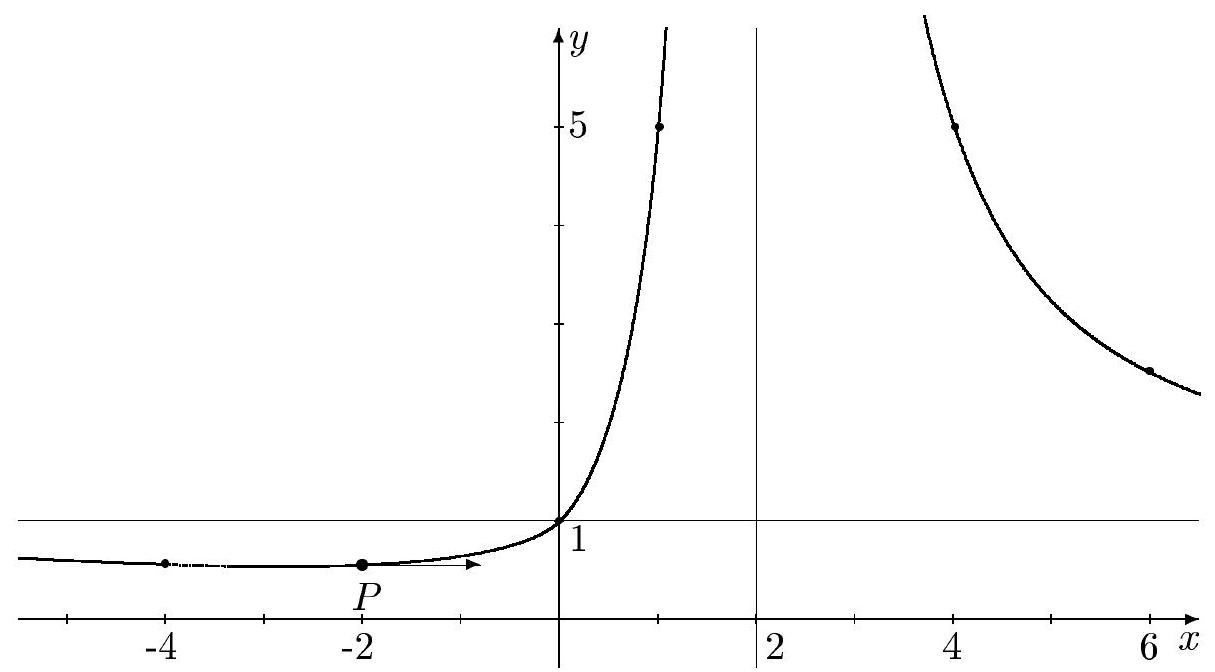
\includegraphics[max width=\textwidth, center]{2024_11_16_fe5b564401bf7db98894g-059}

Rys. 6\\
9.8. $y=10 x-16, y=-\frac{5}{4} x-\frac{1}{4}, y=-\frac{38}{25} x+\frac{16}{125}$.\\
10.2. $V=-\frac{\pi}{6} l^{3} \sin 4 \alpha \cos 2 \alpha, \varphi=3 \pi-4 \alpha, \alpha \in\left(\frac{\pi}{2}, \frac{3 \pi}{4}\right)$.\\
10.3. Dziedzina jest przedział $[0,4]$, a zbiorem wartości przedziat $\left[0, \frac{3}{2}\right]$.\\
10.4. $\frac{240}{1771} \approx 0,136$.\\
10.5. $\left(\frac{1}{4}, \frac{1}{2}\right) \cup[2,4]$.\\
10.6. $S(r)=r\left(1-r^{2}\right)^{3 / 2}, \quad r \in(0,1)$. Wartość największa $\frac{3 \sqrt{3}}{16}$ dla $r=\frac{1}{2}$.\\
10.7. Układ ma cztery rozwiązania:

$$
\left\{\begin{array} { l } 
{ x _ { 1 } = 0 } \\
{ y _ { 1 } = 0 }
\end{array} \left\{\begin{array} { l } 
{ x _ { 2 } = \frac { 1 6 } { 5 } } \\
{ y _ { 2 } = \frac { 1 2 } { 5 } , }
\end{array} \left\{\begin{array} { l } 
{ x _ { 3 } = - \frac { 1 6 } { 5 } } \\
{ y _ { 3 } = - \frac { 1 2 } { 5 } }
\end{array} \left\{\begin{array}{l}
x_{4}=4 \\
y_{4}=-2
\end{array}\right.\right.\right.\right.
$$

Pierwsze równanie przedstawia dwa okręgi styczne do osi $O y$ o środkach $S_{1}\left(\frac{5}{2}, 0\right), \quad S_{2}\left(-\frac{5}{2}, 0\right)$ i promieniu $\frac{5}{2}$. Drugie równanie przedstawia dwie proste równoległe.\\
10.8. Rozwiązania równania: $\frac{3 \pi}{8}, \frac{7 \pi}{8}$. Zbiór rozwiązań nierówności: $\left[0, \frac{3 \pi}{8}\right) \cup\left(\frac{7 \pi}{8}, \pi\right]$.\\
11.1. $\frac{\pi}{6}$.\\
11.2. $\frac{2 \sqrt{6}}{3} R$.\\
11.3. $4,-4$.\\
11.4. $\left(\frac{\pi}{4}, \frac{3 \pi}{4}\right) \cup\left(\frac{5 \pi}{4}, \frac{7 \pi}{4}\right)$.\\
11.6. $|y|=\frac{(x+2)^{2}}{4}-1, \quad x \in(-\infty,-4) \cup(0, \infty)$.\\
11.7. $3^{\sqrt{11}}, 3^{-\sqrt{11}}$.\\
11.8. $[-5,0) \cup(5,6]$.\\
12.1. $\frac{9-\sqrt{5}}{2}$.\\
12.2. -1 .\\
12.3. $\frac{107}{128} \approx 0,836$.\\
12.4. $(x-1)^{2}+(y-1)^{2}=1,(x-6)^{2}+(y-6)^{2}=36,(x+2)^{2}+(y-2)^{2}=4$, $(x-3)^{2}+(y+3)^{2}=9$.\\
12.5. $\frac{2}{3} d^{3} \frac{\operatorname{tg}^{3} \alpha}{\sqrt{\operatorname{tg}^{2} \alpha-1}}, \alpha \in\left(\frac{\pi}{4}, \frac{\pi}{2}\right)$.\\
12.6. $s+\frac{16 P r}{\sqrt{16 P^{2}+s^{4}}}$. Warunek rozwiązalności $r \geq \frac{\sqrt{16 P^{2}+s^{4}}}{4 s}$.\\
12.7. Dla parametrów $p$ różnych od $2 \mathrm{i}-1$ jedno rozwiązanie $x=3 p$, $y=-3 p-2$. Dla $p=2$ nieskończenie wiele rozwiazań spełniajacych warunek $2 x+y-4=0$, gdzie $x$ dowolne rzeczywiste. Dla $p=-1$ nieskończenie wiele rozwiazzań spełniających warunek $x-y+4=0$, gdzie $x$ dowolne rzeczywiste. Rozwiązania o współrzędnych całkowitych:

$$
\begin{gathered}
\left\{\begin{array}{l}
x=-2 \\
y=2
\end{array}, p=-1 ;\left\{\begin{array}{l}
x=-2 \\
y=0
\end{array}, p=-\frac{2}{3} ;\left\{\begin{array}{l}
x=-1 \\
y=-1
\end{array}, p=-\frac{1}{3} ;\right.\right.\right. \\
\left\{\begin{array}{l}
x=0 \\
y=-2
\end{array}, p=0 ;\left\{\begin{array}{l}
x=1 \\
y=2
\end{array}, p=2 ;\left\{\begin{array}{l}
x=2 \\
y=0
\end{array}, p=2 .\right.\right.\right.
\end{gathered}
$$

12.8. $S(y)=\pi\left(y+\frac{3}{2}\right) \sqrt{1+\left(y-\frac{3}{2}\right)^{2}}, \quad y \in\left[0, \frac{3}{2}\right]$. Wartość najmniejsza $\frac{3 \sqrt{13}}{4} \pi$ dla $y=0$.\\
13.2. 3.\\
13.3. $f(m)=\left|2^{-(m-3)}-2\right|, \quad m \in(-\infty, 4] \backslash\left\{\log _{2} 7\right\}$. Wykres funkcji $f$ przedstawiono na rysunku 7 .\\
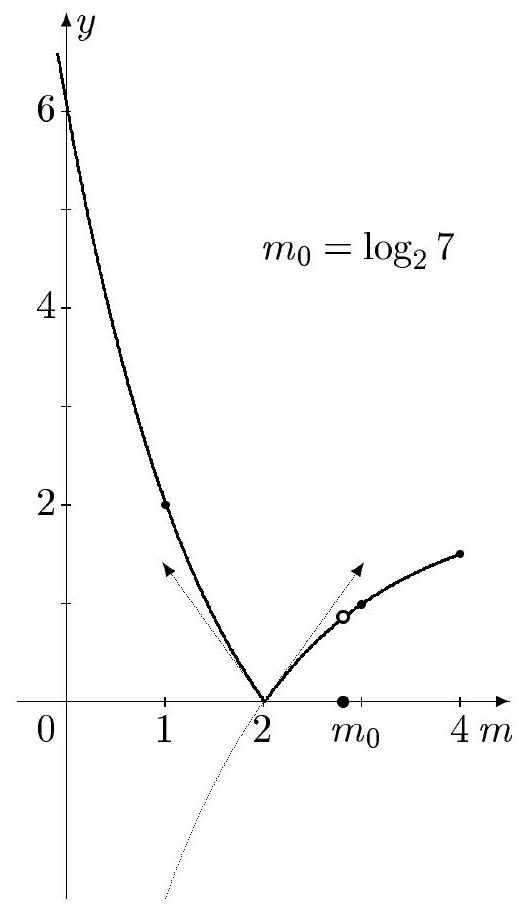
\includegraphics[max width=\textwidth, center]{2024_11_16_fe5b564401bf7db98894g-061}

Rys. 7\\
13.4. $\frac{35}{144} \approx 0,243$.\\
13.5. $10,8,6,4$ lub $10,8,6,4,2,0,-2$ lub $-20,-12,-4,4,12$, 20, 28.\\
13.6. $\frac{10}{27}$.\\
13.7. $Q\left(2+\frac{2}{5} \sqrt{5}, \frac{4}{5} \sqrt{5}\right)$. Zbiory $A, B$ oraz $A \cap B$ przedstawiono na rysunku 8.\\
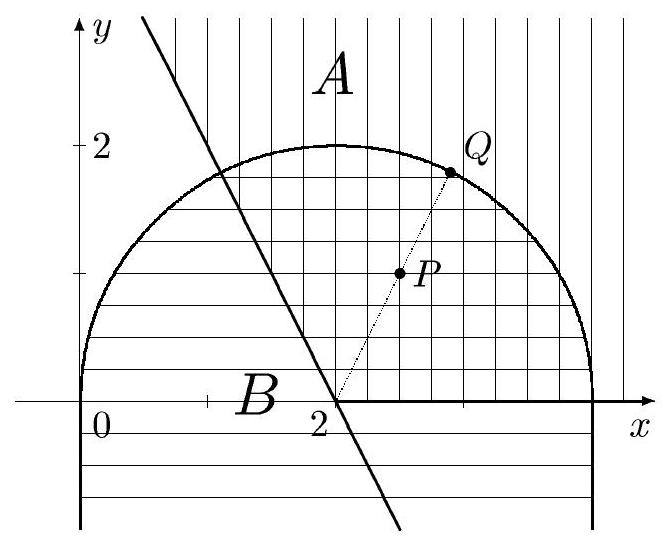
\includegraphics[max width=\textwidth, center]{2024_11_16_fe5b564401bf7db98894g-062}

Rys. 8\\
13.8. Funkcja jest parzysta. $D=[-\sqrt{8}, \sqrt{8}]$; miejsca zerowe -2 i 2 ; maksima lokalne $\frac{1}{2}$ dla $x=-\sqrt{7}$ oraz dla $x=\sqrt{7}$; minimum lokalne\\
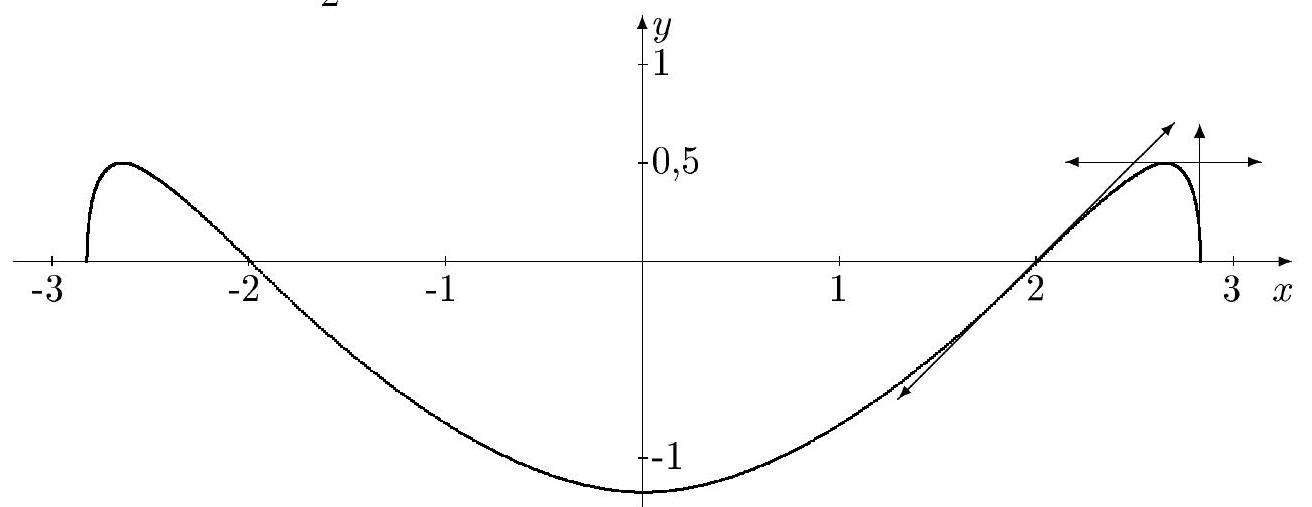
\includegraphics[max width=\textwidth, center]{2024_11_16_fe5b564401bf7db98894g-062(1)}

Rys. 9\\
$-4+\sqrt{8}$ dla $x=0$; funkcja rosnaca w $(-\sqrt{8},-\sqrt{7})$ oraz w $(0, \sqrt{7})$; malejaca $\mathrm{w}(-\sqrt{7}, 0)$ oraz w $(\sqrt{7}, \sqrt{8})$; wypukła w $(-2,2)$; wklęsła w $(-\sqrt{8},-2)$ oraz $\mathrm{w}(2, \sqrt{8})$; punkty przegięcia $(-2,0),(2,0)$, proste $x=-\sqrt{8}$ oraz $x=\sqrt{8}$ styczne do wykresu funkcji. Wykres funkcji przedstawiono na rysunku 9.\\
14.1. 9.\\
14.2. $2 \pi(3+2 \sqrt{3})$.\\
14.3. a) $m=-\frac{1}{2}$; b) $m=\frac{4}{3}$; c) $m=0$ lub $m=2 \sqrt{3}$.\\
14.5. Elipsa o równaniu $\frac{x^{2}}{36}+\frac{(y-1)^{2}}{4}=1$, środku $S(0,1)$ i półosiach $a=6, b=2$. Pole figury wynosi $8 \pi-6 \sqrt{3}$.\\
14.6. $+\infty$.\\
14.7. a) $\frac{1}{20}$; b) $\frac{7}{20}$.\\
14.8. $\frac{\sqrt{2}-\cos \alpha}{2 \sin \alpha} a, \alpha \in\left(0, \frac{\pi}{2}\right)$.\\
15.1. $12 \mathrm{~km} / \mathrm{h}, 15 \mathrm{~km} / \mathrm{h}, A B=27 \mathrm{~km}$.\\
15.2. $(-\infty,-\sqrt{3}] \cup(2, \infty)$.\\
15.3. $108 \sqrt{3} \mathrm{~m}^{2}, \frac{405}{4} \sqrt{3} \mathrm{~m}^{3}$.\\
15.4. $w_{n}=1600+\frac{8000}{3}\left(\left(\frac{203}{200}\right)^{n-1}-1\right)$, pensja w kwietniu 2002 roku wynosi $1806,09 \mathrm{zl}$, średnia pensja w 2002 roku wynosi 1827,96 zł.\\
15.5. $f^{-1}(x)=\sqrt[3]{x}, \quad x \in \mathbf{R}$. Wykres funkcji $h$ przedstawiono na rysunku 10.\\
15.6. $\frac{\pi}{12}+k \frac{\pi}{3}, k \in \mathbf{Z}$.\\
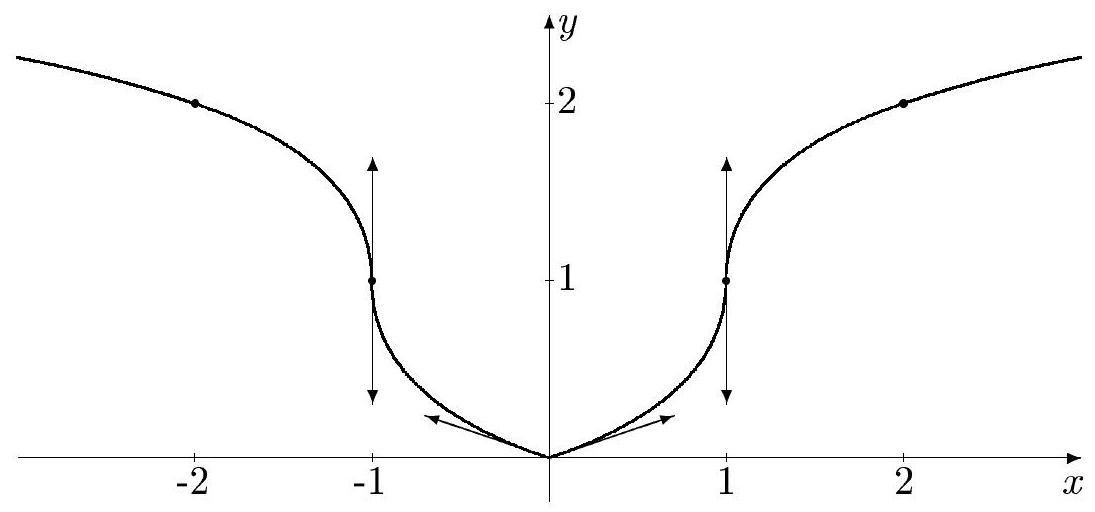
\includegraphics[max width=\textwidth, center]{2024_11_16_fe5b564401bf7db98894g-064(1)}

Rys. 10\\
15.7. $\frac{9}{85} \sqrt{85}$.\\
15.8. $f(x)=\frac{x^{2}-x}{x-2}=x+1+\frac{2}{x-2} ; D=(-\infty, 0] \cup(2, \infty) ;$ asymptota pionowa prawostronna $x=2$; asymptota ukośna obustronna $y=x+1$; minimum lokalne $3+2 \sqrt{2}$ dla $x_{0}=2+\sqrt{2}$; funkcja rosnaca w $(-\infty, 0)$ oraz w $(2+\sqrt{2}, \infty)$; malejaca w $(2,2+\sqrt{2})$; wypukła w $(2, \infty)$; wklęłła w $(-\infty, 0)$. Wykres funkcji przedstawiono na rysunku 11.\\
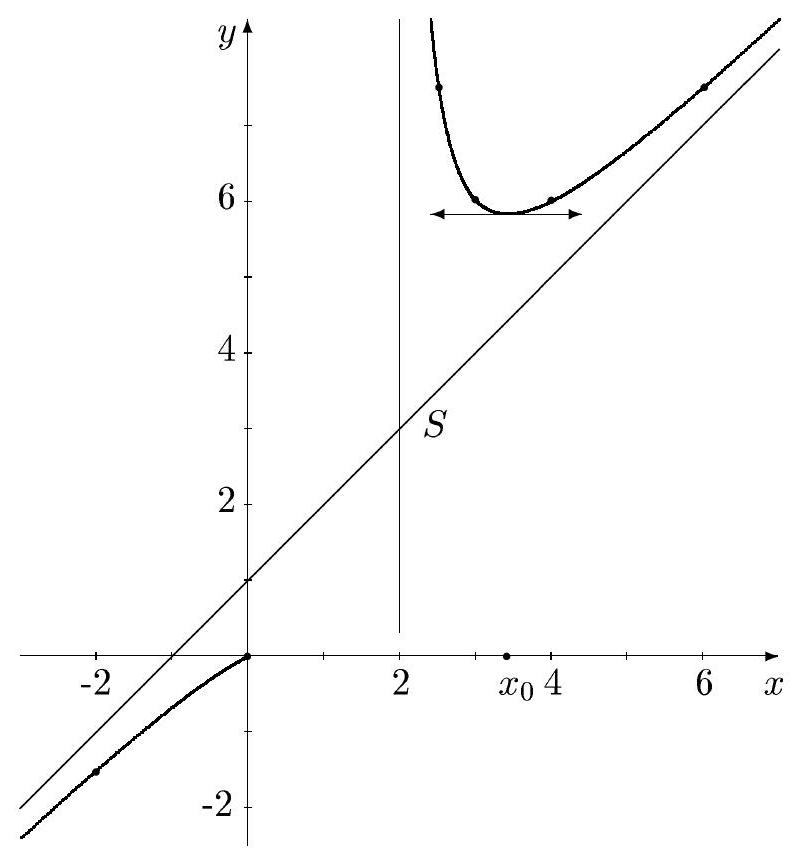
\includegraphics[max width=\textwidth, center]{2024_11_16_fe5b564401bf7db98894g-064}

Rys. 11\\
16.1. Cena mniejsza od poczatkowej o $2,25 \%$.\\
16.2. Zbiór składa się z łuków czterech okręgów oraz punktu $(0,0)$ i jest przedstawiony na rysunku 12.\\
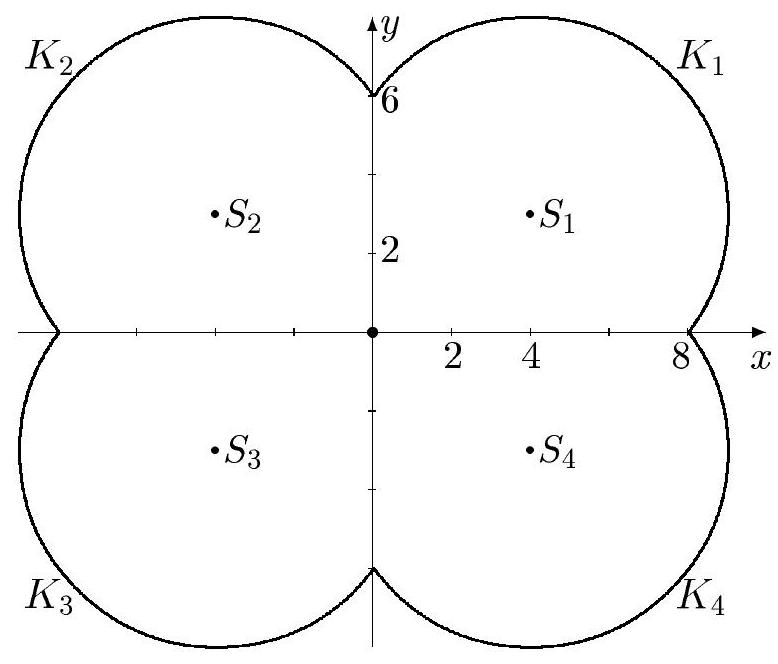
\includegraphics[max width=\textwidth, center]{2024_11_16_fe5b564401bf7db98894g-065}

Rys. 12\\
16.3. $18 h^{2} \frac{\sin ^{2} \alpha}{\sin 3 \alpha}, \alpha \in\left(0, \frac{\pi}{3}\right)$.\\
16.4. 18 cm od wierzchołka kąta rozwartego, $\alpha=38^{\circ} 13^{\prime}$.\\
16.5. $\sqrt{2}, \frac{\sqrt{2}}{2}$.\\
16.6. Dziedziną jest $\mathbf{R}$, a zbiorem wartości przedzial $[3-\sqrt{5}, 3+\sqrt{5}]$.\\
16.7. $(-1,0] \cup\left\{\frac{\sqrt{17}-1}{2}\right\}$.\\
16.8. 2.\\
17.1. $1,-1, \sqrt{\frac{\sqrt{17}-1}{8}},-\sqrt{\frac{\sqrt{17}-1}{8}}$; wyraz czwarty 0 lub $\frac{9-\sqrt{17}}{4}$.\\
17.2. $\frac{16}{35} \approx 0,457$.\\
17.4. $x^{2}+\left(y-r^{2}-\frac{1}{4}\right)^{2}=r^{2}$. Rozwiązanie istnieje dla $r>\frac{1}{2}$.\\
17.6. $\left[\frac{1}{3}, \frac{\sqrt{6}}{6}\right)$.\\
17.7. $\frac{3 d\left(c^{2}+d^{2}\right)}{2 c^{2}} \sqrt{c^{2}-d^{2}}$ lub $\frac{3 d\left(2 c^{2}-d^{2}\right)}{2 c^{2}} \sqrt{c^{2}-d^{2}}, \quad c>d$.\\
17.8. Gdy w równoległościanie sa dwa wierzchołki trójścienne o trzech kątach płaskich $\beta$, to objętość wynosi $2 a^{3} \sqrt{\sin \frac{3}{2} \beta \sin ^{3} \frac{1}{2} \beta}$. Gdy $\beta \in\left(\frac{\pi}{3}, \frac{\pi}{2}\right)$ i w równoległościanie sa dwa wierzchołki trójścienne o trzech kątach płaskich $\pi-\beta$, to objętość wynosi $2 a^{3} \sqrt{-\cos \frac{3}{2} \beta \cos ^{3} \frac{1}{2} \beta}$.\\
18.1. $\frac{3}{2}$.\\
18.2. $3 x-2 y+1=0$.\\
18.3. $V=-\frac{\pi}{6} l^{3} \sin 4 \alpha \cos 2 \alpha, \varphi=3 \pi-4 \alpha, \alpha \in\left(\frac{\pi}{2}, \frac{3 \pi}{4}\right)$.\\
18.4. Niech $x$ oznacza cenę długopisu, a $y$ cenę zeszytu. Dla $k \neq 2$ jest $x=\frac{5 k+2}{2 k+2}, \quad y=\frac{k}{k+2}$. Dla $k=2$ spełniona jest relacja $2 x+4 y=5$. Ceny długopisu i zeszytu moga być następujące:

$$
\begin{gathered}
\left\{\begin{array}{l}
x=2,3 \\
y=0,9 ;
\end{array} ;\left\{\begin{array} { l } 
{ x = 2 , 1 } \\
{ y = 0 , 8 ; }
\end{array} \quad \left\{\begin{array}{l}
x=1,7 \\
y=0,6 ;
\end{array} ;\left\{\begin{array}{l}
x=1,5 \\
y=0,5 ;
\end{array}\right.\right.\right.\right. \\
\left\{\begin{array} { l } 
{ x = 1 , 3 } \\
{ y = 0 , 6 ; }
\end{array} \quad \left\{\begin{array} { l } 
{ x = 1 , 1 } \\
{ y = 0 , 7 }
\end{array} \quad \left\{\begin{array}{l}
x=0,9 \\
y=0,8 .
\end{array}\right.\right.\right.
\end{gathered}
$$

18.5. $\left[-\frac{\pi}{4}+k \pi, k \pi\right] \cup\left[\frac{\pi}{4}+k \pi, \frac{\pi}{2}+k \pi\right), k \in \mathbf{Z}$.\\
18.6. $\frac{496}{729} \approx 0,680 ; \quad$ о $\frac{496}{728 \cdot 729} \approx 0,001$.\\
18.7. $2-\frac{4}{3} \sqrt{2}$.\\
18.8. $6 \sqrt{2}-4$.\\
19.1. $\frac{31}{8}$.\\
19.2. $12+24 \sqrt{2} \mathrm{~cm}$.\\
19.3. $s \leq 20$.\\
19.4. $\frac{3}{2} \sqrt{55}$ arów. Plan działki w skali 1:1000 przedstawia rysunek 13 .\\
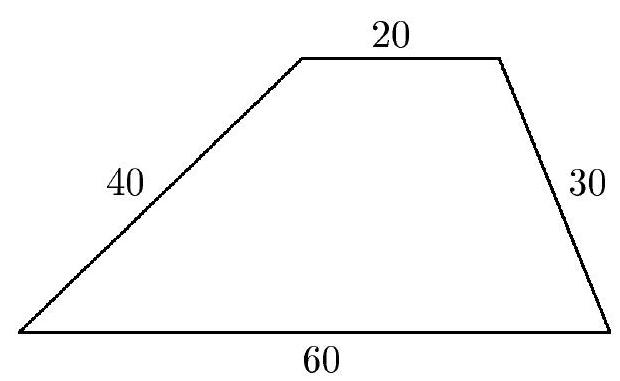
\includegraphics[max width=\textwidth, center]{2024_11_16_fe5b564401bf7db98894g-067}

Rys. 13\\
19.5. Wartość największa 6 dla $m=0$.\\
19.7.

$$
\left\{\begin{array} { l } 
{ x _ { 1 } = \frac { 5 \pi } { 1 2 } } \\
{ y _ { 1 } = \frac { \pi } { 1 2 } , }
\end{array} \left\{\begin{array} { l } 
{ x _ { 2 } = \frac { \pi } { 1 2 } } \\
{ y _ { 2 } = \frac { 5 \pi } { 1 2 } , }
\end{array} \left\{\begin{array} { l } 
{ x _ { 3 } = - \frac { 7 \pi } { 1 2 } } \\
{ y _ { 3 } = - \frac { 1 1 \pi } { 1 2 } , }
\end{array} \left\{\begin{array}{l}
x_{4}=-\frac{11 \pi}{12} \\
y_{4}=-\frac{7 \pi}{12}
\end{array}\right.\right.\right.\right.
$$

19.8. $1,1, \frac{\sqrt{3}}{2}, \frac{2 \sqrt{7}}{7}, \frac{\sqrt{42}}{7}, \frac{\sqrt{42}}{7}$.\\
20.1. $-1,1,2$.\\
20.2. $\frac{8}{5}(2-\sqrt{3})$.\\
20.3. $\frac{50}{81} \approx 0,617$.\\
20.4. Częśćć elipsy o równaniu $\frac{x^{2}}{\frac{5}{3}}+\frac{(y-5)^{2}}{\frac{5}{2}}=1$ dla $y \leq 6$.\\
20.5. Asymptota pionowa obustronna $x=1$; asymptota pozioma lewostronna $y=-1$; asymptota pozioma prawostronna $y=1$. Wykres funkcji przedstawiono na rysunku 14.\\
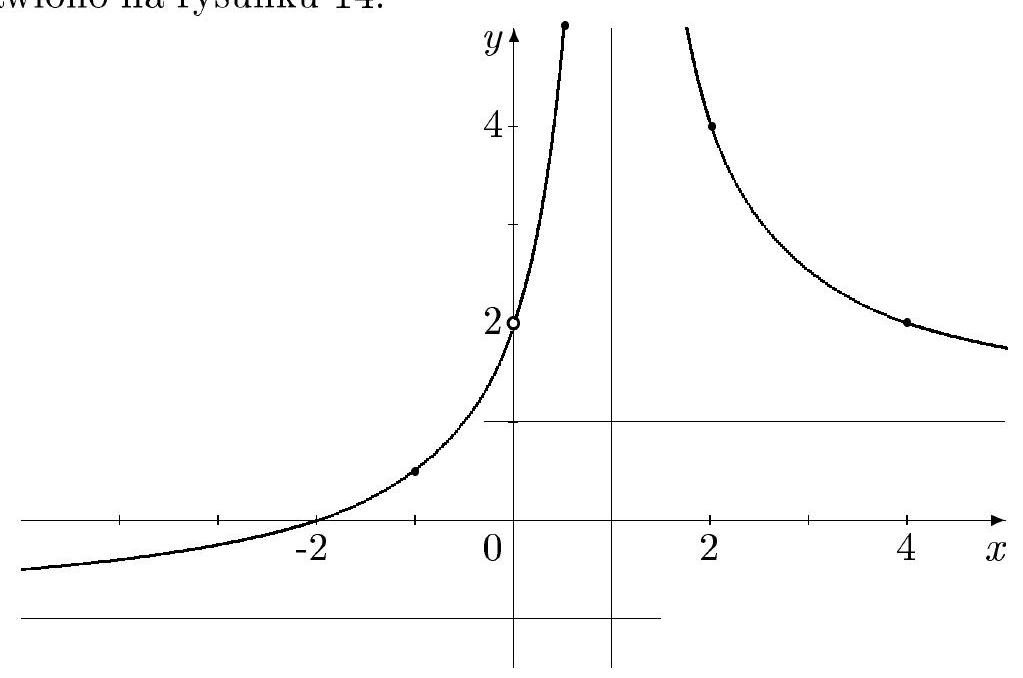
\includegraphics[max width=\textwidth, center]{2024_11_16_fe5b564401bf7db98894g-068}

Rys. 14\\
20.6. $(-\infty,-1] \cup\left[-\frac{1}{2}, 0\right) \cup(0,1]$.\\
20.7. $-\sqrt{8}$ lub $\sqrt{8}$.\\
21.1. O $5 \mathrm{~cm}^{2}$.\\
21.2. $\frac{3}{4}$.\\
21.3. $\frac{4-\sqrt{2}}{6}, \frac{4+\sqrt{2}}{6}$.\\
21.4. Granica ciagu wynosi $\frac{1}{2}$.\\
21.5. $(-\pi+4 k \pi, \pi+4 k \pi), k \in \mathbf{Z}$.\\
21.6. -1.\\
21.7. $r=\frac{2 \sqrt{2}}{3} R, \quad h=\frac{4}{3} R$.\\
21.8. $y=1-(4+2 \sqrt{5})(x-2), \quad y=1-(4-2 \sqrt{5})(x-2)$.\\
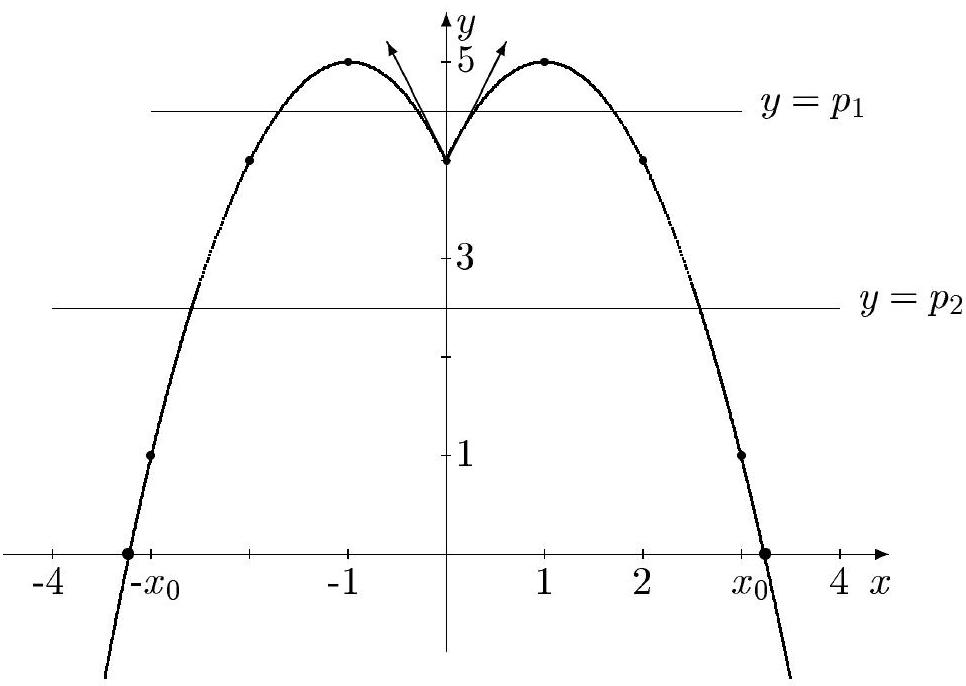
\includegraphics[max width=\textwidth, center]{2024_11_16_fe5b564401bf7db98894g-069}

Rys. 15\\
22.1. Wykres funkcji przedstawiono na rysunku 15 , gdzie $x_{0}=1+\sqrt{5}$. Niech $f(p)$ oznacza liczbę rozwiązań równania $4+2|x|-x^{2}=p$. Wtedy

$$
f(p)=\left\{\begin{array}{lll}
0 & \text { dla } & p>5, \\
2 & \text { dla } & p<4 \text { lub } p=5, \\
3 & \text { dla } & p=4 \\
4 & \text { dla } & 4<p<5
\end{array}\right.
$$

22.2. 117 minut; 5475,6 m³.\\
22.3. Średnice podstaw $6+2 \sqrt{5} \mathrm{~cm}$ oraz $6-2 \sqrt{5} \mathrm{~cm}$; tworzaca 6 cm .\\
22.4. Gdy kąt $\alpha$ jest ostry i $\sin \alpha<\frac{4}{5}$, wówczas są dwa rozwiązania: $P_{1}=\frac{8}{25} R^{2}(4 \cos \alpha-3 \sin \alpha) \sin \alpha$ oraz $P_{2}=\frac{8}{25} R^{2}(4 \cos \alpha+3 \sin \alpha) \sin \alpha$.

Jeśli $\sin \alpha \geq \frac{4}{5}$, to jest jedno rozwiązanie $P_{2}$, a jeśli $\alpha$ rozwarty i $\sin \alpha<\frac{4}{5}$, to brak rozwiąań.\\
22.5. $\left(0, \frac{1}{4}\right] \cup[16, \infty)$.\\
22.6. $\cos \alpha=\frac{\sqrt{7}}{14}$, obwód $\frac{1}{6}(9+\sqrt{12}+\sqrt{21}) a$.\\
22.7. $\frac{\pi}{4}+k \frac{2 \pi}{3}, k \in \mathbf{Z}$.\\
22.8. $\sqrt{2} x+2 y-3=0$.\\
23.1. Tak. W obu przypadkach liczba ,słów" wynosi 210.\\
23.2. $-3,-1,1$.\\
23.3. $\frac{3}{8} a$.\\
23.4. $\frac{1}{12} b^{2}(3 a-b) \operatorname{tg} \alpha$.\\
23.5. $[-\sqrt{5}, 0) \cup(1,2)$.\\
23.7. Punkt $Q(1,1)$.\\
23.8. $\left(\frac{5 \pi}{4}+2 k \pi, \frac{3 \pi}{2}+2 k \pi\right) \cup\left(\frac{3 \pi}{2}+2 k \pi, \frac{7 \pi}{4}+2 k \pi\right), k \in \mathbf{Z}$.\\
24.1. $2+\frac{3}{2} \sqrt{2}$.\\
24.2. $\frac{7}{18} \approx 0,389$.\\
24.3. Dla $m \neq 10$ jedno rozwiązanie $x=\frac{m}{m-10}, \quad y=\frac{m-15}{m-10}$. Dla $m=10$ układ sprzeczny. Rozwiązania tworzą prosta $x+2 y-3=0 \mathrm{bez}$ punktu $P(1,1)$.\\
24.4. $\sqrt{\frac{6-6 \cos \alpha}{5-4 \cos \alpha}}, \alpha \in\left(0, \frac{\pi}{3}\right)$.\\
24.5. $\left(-\infty, \frac{1}{2}\right] \cup\left[\frac{3}{2}, \infty\right)$.\\
24.7. Równanie prostej $k: x+2 y-8=0$. Równania stycznych tworzacych z $k$ kat $45^{\circ}: x-3 y+2+5 \sqrt{2}=0, x-3 y+2-5 \sqrt{2}=0$, $3 x+y-4+5 \sqrt{2}=0,3 x+y-4-5 \sqrt{2}=0$.\\
24.8. $a=3, \quad b=32$. Styczna $y=-3 x+13$. Wykres funkcji przedstawiono na rysunku 16.\\
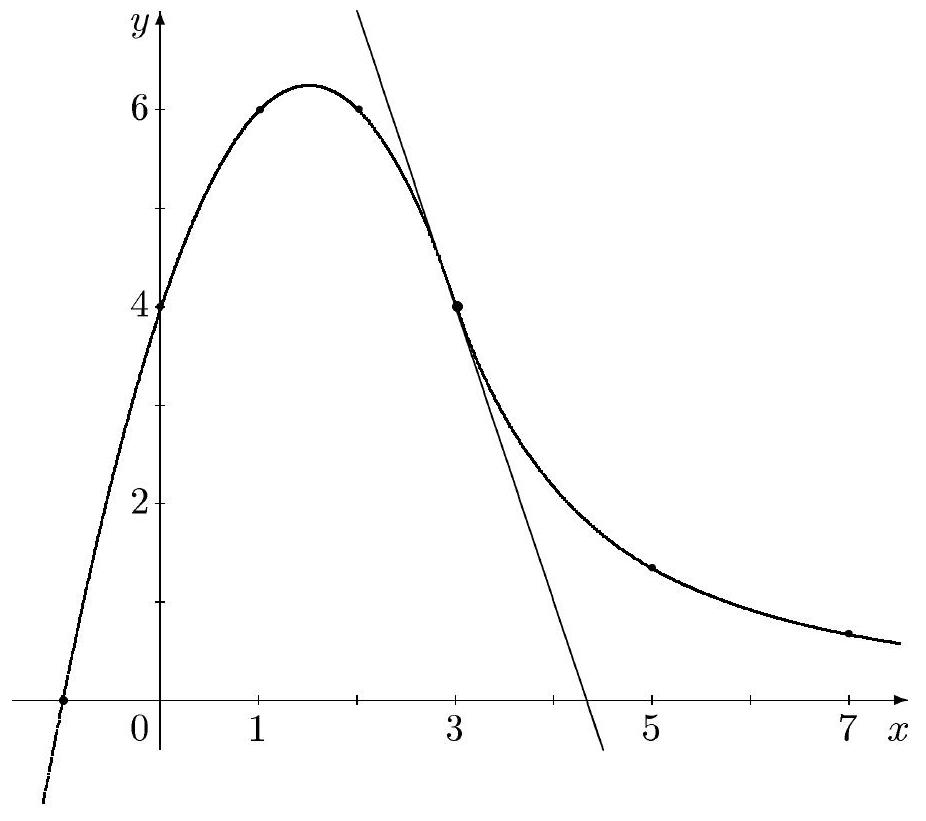
\includegraphics[max width=\textwidth, center]{2024_11_16_fe5b564401bf7db98894g-071}

Rys. 16\\
25.1. $-\frac{1}{6}, 0, \frac{1}{2}$.\\
25.2. $S(x)=x(a-x), \quad x \in(0, a)$. Wartość największa $\frac{a^{2}}{4}$ dla $x=\frac{a}{2}$.\\
25.3. Rysunek 17.\\
25.4. Elipsa o równaniu $\frac{(x-4)^{2}}{25}+\frac{y^{2}}{9}=1$ oraz część prostej $y=0$ dla $x>9$.\\
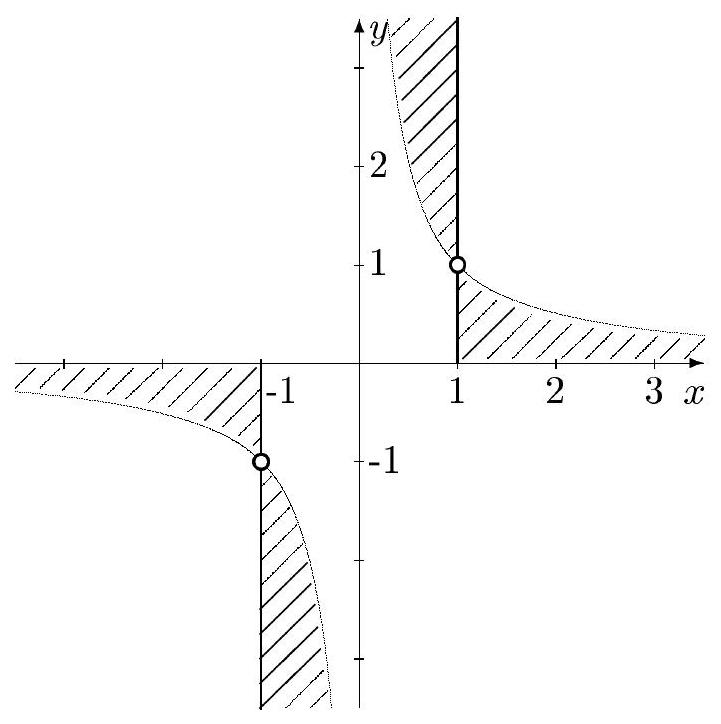
\includegraphics[max width=\textwidth, center]{2024_11_16_fe5b564401bf7db98894g-072}

Rys. 17\\
25.5. $\frac{5}{12} \approx 0,417$.\\
25.7. $D=[1,5)$; asymptota pionowa lewostronna $x=5$; funkcja rosnąca w $(1,5)$; wypukła w $(2,5)$; wklęsła w $(1,2)$; punkt przegięcia $P(2,1)$; prosta $x=1$ styczna do wykresu funkcji. Wykres funkcji przedstawiono na rysunku 18.\\
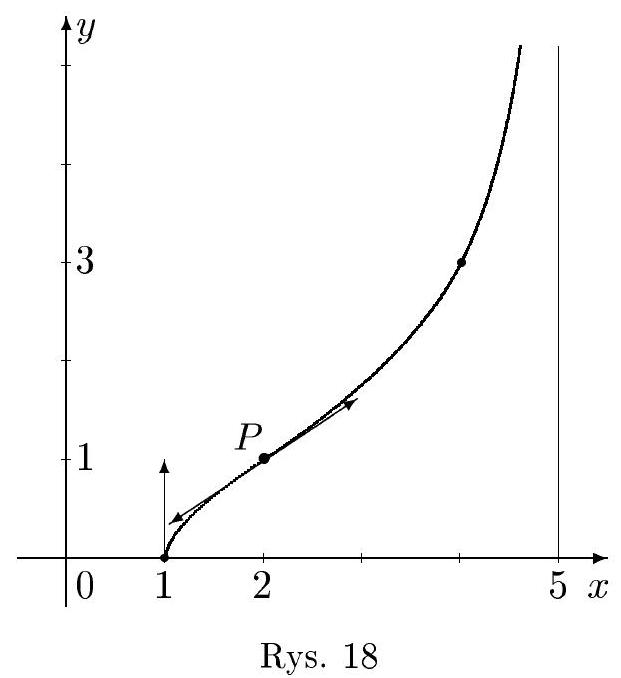
\includegraphics[max width=\textwidth, center]{2024_11_16_fe5b564401bf7db98894g-072(1)}\\
25.8. $2 a \cos \alpha(1+2 \cos \alpha), \alpha \in\left(0, \frac{\pi}{3}\right)$.\\
26.1. $30(\pi+\sqrt{3}) \mathrm{cm}$.\\
26.2. 213 zł i 85 gr.\\
26.3. $4 x-7 y+17=0$; pole $\frac{10}{3}$.\\
26.4. $\frac{\sqrt{2}}{3} r^{3} \frac{(1+\sin \alpha) \cos \frac{\beta}{2} \operatorname{ctg} \frac{\alpha}{2}}{\cos \alpha \sqrt{-\cos \beta}}, \beta \in\left(\frac{\pi}{2}, \pi\right)$.\\
26.5. Maksimum lokalne 2 dla $x=0$. Wykres funkcji przedstawiono na rysunku 19.\\
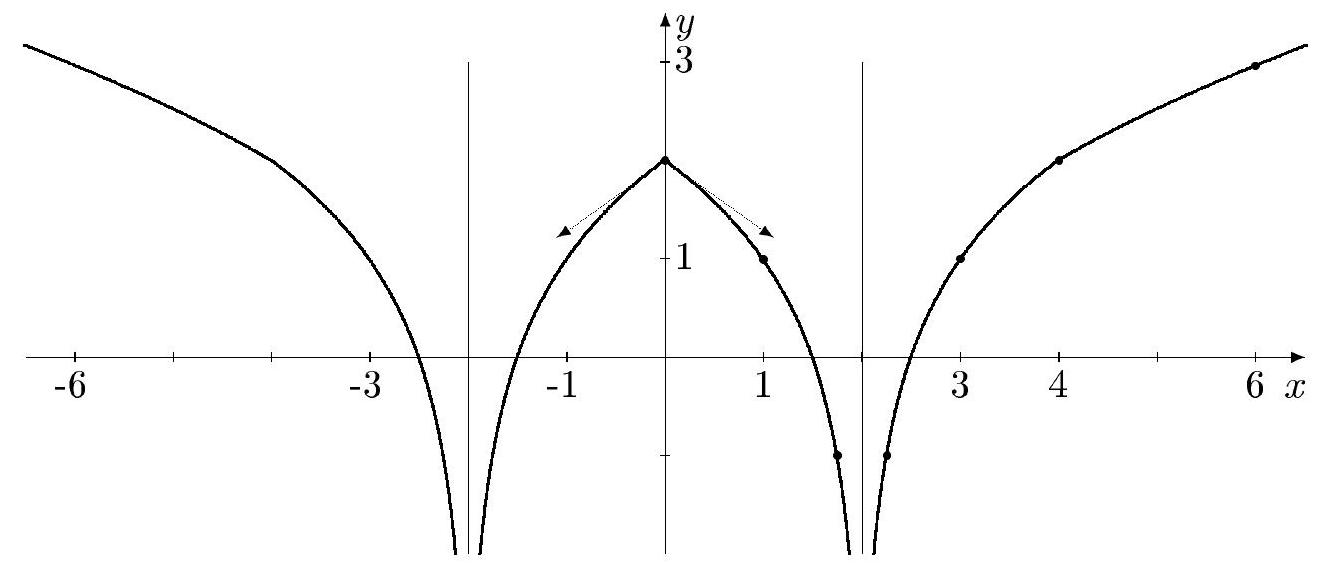
\includegraphics[max width=\textwidth, center]{2024_11_16_fe5b564401bf7db98894g-073}

Rys. 19\\
26.6. $\frac{\pi}{3}+k \frac{\pi}{2}, k \in \mathbf{Z}$.\\
26.7. Dla $a \in[0,4)$. Wtedy

$$
g(x)=\left\{\begin{array}{lll}
-x^{4} & \text { dla } a=0, \\
\frac{x^{4}}{a^{3} x^{3}-\left(a^{2}+a\right) x^{2}+2 a x-1} & \text { dla } \quad 0<a<4 .
\end{array}\right.
$$

Dla $a=3$ asymptota pionowa obustronna $x=\frac{1}{3}$, asymptota ukośna obustronna $3 x-27 y+4=0$.\\
26.8. $S(y)=\pi(y+3) \sqrt{4+(y-3)^{2}}, \quad y \in[0,3]$. Wartość najmniejsza dla $y=0$ wynosząca $3 \pi \sqrt{13}$.\\
27.1. $p \in[-2,2]$.\\
27.2. $\left(x-\frac{8}{5}\right)^{2}+\left(y-\frac{9}{5}\right)^{2}=\frac{16}{5}$.\\
27.3. $\frac{\sqrt{16 r^{2} \sin ^{2} \alpha-d^{2}}}{2 \sin \alpha}, 4 r \sin \alpha \cos \alpha<d<4 r \sin \alpha$.\\
27.4. $2 S^{3 / 2} \sqrt[4]{\frac{18\left(\operatorname{ctg}^{2} \beta-1\right)^{2}}{\left(17+\operatorname{ctg}^{2} \beta\right)^{3}}}$.\\
27.5. $-\infty$.\\
27.6. $\left(2 k \pi, \frac{\pi}{6}+2 k \pi\right], k \in \mathbf{Z}$.\\
27.7. $\frac{425}{768} \approx 0,553$.\\
27.8. Tangens kąta przecięcia linii wynosi $\frac{9}{37}$. Szukany zbiór pokazano na rysunku 20.\\
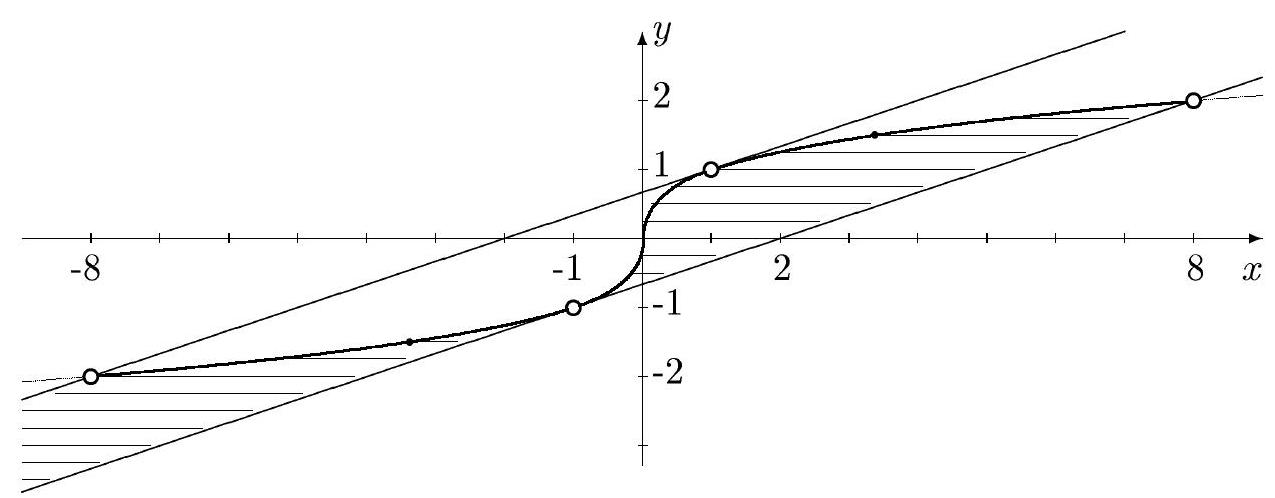
\includegraphics[max width=\textwidth, center]{2024_11_16_fe5b564401bf7db98894g-074}

Rys. 20\\
28.1. $\frac{13}{9}$.\\
28.2. $p \in\left[\frac{5}{4}, \frac{\sqrt{7}}{2}\right)$.\\
28.3. $\frac{d^{2}-r^{2}}{2} \operatorname{tg} \frac{\alpha}{2}, \quad r<d$.\\
28.4. $\frac{2 R}{R+r} \sqrt{3 R r}$.\\
28.5. Trzy pierwiastki, w tym jeden ujemny i dwa dodatnie.\\
28.7. $\frac{2 \pi}{3}+2 k \pi \operatorname{lub} \frac{4 \pi}{3}+2 k \pi, \quad k \in \mathbf{Z}$.\\
28.8. Szukana krzywa jest parabola o równaniu $y=2 x^{2}+\frac{1}{2}$ bez punktu $W\left(0, \frac{1}{2}\right)$.\\
29.1. 15.\\
29.2. 307692.\\
29.3. $c(\cos \alpha-\cos 2 \alpha), \alpha \in\left(0, \frac{\pi}{4}\right)$.\\
29.4. $(-\infty,-\sqrt{2}] \cup(-1,0) \cup(0,2) \cup[1+\sqrt{3}, \infty)$.\\
29.5. Rysunek 21.\\
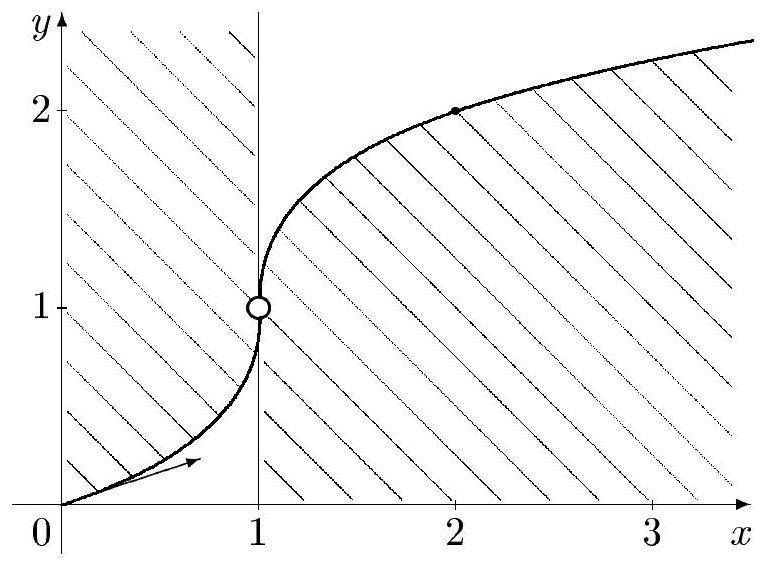
\includegraphics[max width=\textwidth, center]{2024_11_16_fe5b564401bf7db98894g-075}

Rys. 21\\
29.6. $\frac{\pi}{6}+k \frac{\pi}{3}$ lub $k \pi, k \in \mathbf{Z}$.\\
29.7. $-\frac{1}{4}$.\\
29.8. Wartość najmniejsza 0 dla $x=-1$, a wartość największa $\frac{1+\sqrt{2}}{2}$ dla $x=-1+\sqrt{2}$.\\
30.1. $\frac{\sqrt{2}}{2} \frac{V_{1}^{2}}{V_{1}+V_{2}}$, gdzie $V_{1} \geq V_{2}$.\\
30.2. Tak, na dwa sposoby: $3800,6100,8400,10700$ i 13000 zl lub 1000, 3400, 5800, 8200, 10600 i 13000 zł.\\
30.3. Sa cztery takie okręgi i mają równania:\\
$\left(x-\frac{3}{2}\right)^{2}+(y-1-\sqrt{6})^{2}=\frac{9}{4}, \quad\left(x-\frac{3}{2}\right)^{2}+(y-1+\sqrt{6})^{2}=\frac{9}{4}$,\\
$(x+1)^{2}+(y-1)^{2}=1,(x-3)^{2}+(y-1)^{2}=9$.\\
30.4. $\frac{2 k}{k^{2}-1} \sin \beta, k>1$.\\
30.5. 7, 13.\\
30.6. $a=-3, \quad b=1$.\\
30.7. $(-\infty, 0] \cup\left[1, \log _{2} \frac{3+\sqrt{17}}{2}\right]$.\\
30.8. $\left(-\pi,-\frac{2 \pi}{6}\right),\left(-\frac{\pi}{6}, \frac{4 \pi}{6}\right),\left(\frac{5 \pi}{6}, \pi\right)$.\\
31.1. $\frac{136}{4807} \approx 0,028$.\\
31.2. Objęstość ostrosłupa wynosi $\frac{343}{3} \mathrm{~cm}^{3}$, a objętość najmniejszej części $\frac{61}{3} \mathrm{~cm}^{3}$.\\
31.3. Układ ma trzy rozwiązania:

$$
\left\{\begin{array} { l } 
{ x _ { 1 } = 3 + \sqrt { 3 } } \\
{ y _ { 1 } = 3 - \sqrt { 3 } , }
\end{array} \left\{\begin{array} { l } 
{ x _ { 1 } = 3 - \sqrt { 3 } } \\
{ y _ { 1 } = 3 + \sqrt { 3 } , }
\end{array} \left\{\begin{array}{l}
x_{1}=2+2 \sqrt{2} \\
y_{1}=2-2 \sqrt{2}
\end{array}\right.\right.\right.
$$

31.4. $-\frac{1}{2} d^{2} \sin 2 \alpha \operatorname{tg}^{2} \frac{\alpha}{2}, \alpha \in\left(\frac{\pi}{2}, \pi\right)$.\\
31.6. $-\sqrt[3]{4}$.\\
31.7. $B_{1}(5,3), C_{1}(3,2), D_{1}(4,0)$ lub $B_{2}(10,-2), C_{2}(13,2), D_{2}(9,5)$.\\
31.8. $D=(0, \infty)$; asymptota pionowa prawostronna $x=0$; minimum lokalne 2 dla $x=1$; funkcja rosnaca w $(1, \infty)$; malejaca w $(0,1)$, wypukła w $(0,3)$; wklęsła w $(3, \infty)$; punkt przegięcia $P\left(3, \frac{4}{3} \sqrt{3}\right)$; krzywa asymptotyczna $(\mathrm{w}+\infty) y=\sqrt{x}$. Wykres funkcji przedstawiono na rysunku 22.\\
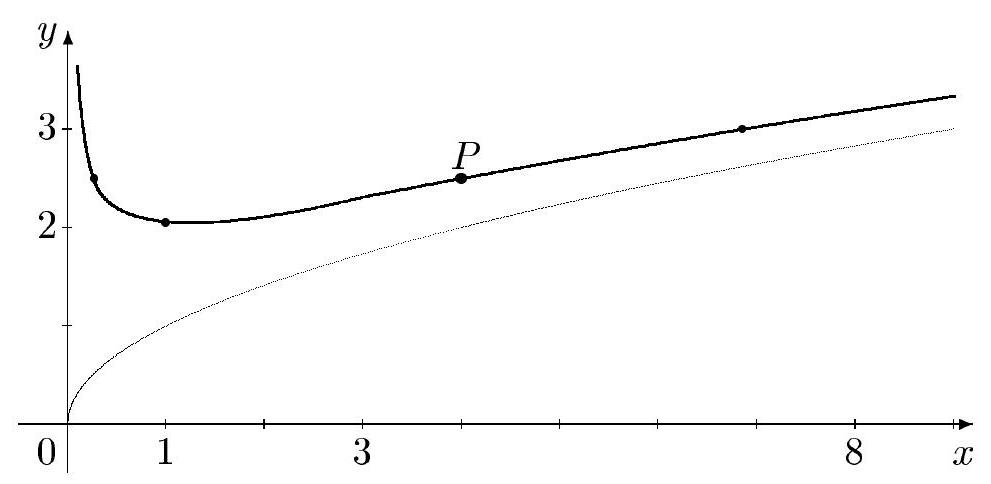
\includegraphics[max width=\textwidth, center]{2024_11_16_fe5b564401bf7db98894g-077}

Rys. 22\\
32.1. 15 dni.\\
32.2. $8, \frac{1}{8}$.\\
32.3. 65,7 litra.\\
32.4. $m \in\left(0, \frac{\sqrt{5}-1}{2}\right)$.\\
32.5. $\frac{2757}{3125} \approx 0,882$.\\
32.6. $\frac{\pi}{4}+k \pi \operatorname{lub} \frac{\pi}{12}+k \pi \operatorname{lub} \frac{5 \pi}{12}+k \pi, k \in \mathbf{Z}$.\\
32.7. $y=-1$ (dwa punkty wspólne), $32 x+27 y-5=0$ (trzy punkty wspólne).\\
32.8. $R=\frac{1}{3} b \sqrt{\frac{9+3 \cos ^{2} \alpha}{2+2 \cos \alpha}}$. Cosinusy katów nachylenia ścian bocznych wynosza $\frac{1}{2}$ oraz $\sqrt{\frac{1-\cos \alpha}{7-\cos \alpha}}$.\\
33.1. Mniejszy o 23,56\%.\\
33.2. Szukaną linię stanowią dwie proste o równaniach $2 x+3 y-1=0$ oraz $4 x-y+5=0$ bez punktu ich przecięcia $P(-1,1)$.\\
33.3. $\frac{7 \pi}{4}$.\\
33.4. $2(7+\sqrt{19})$.\\
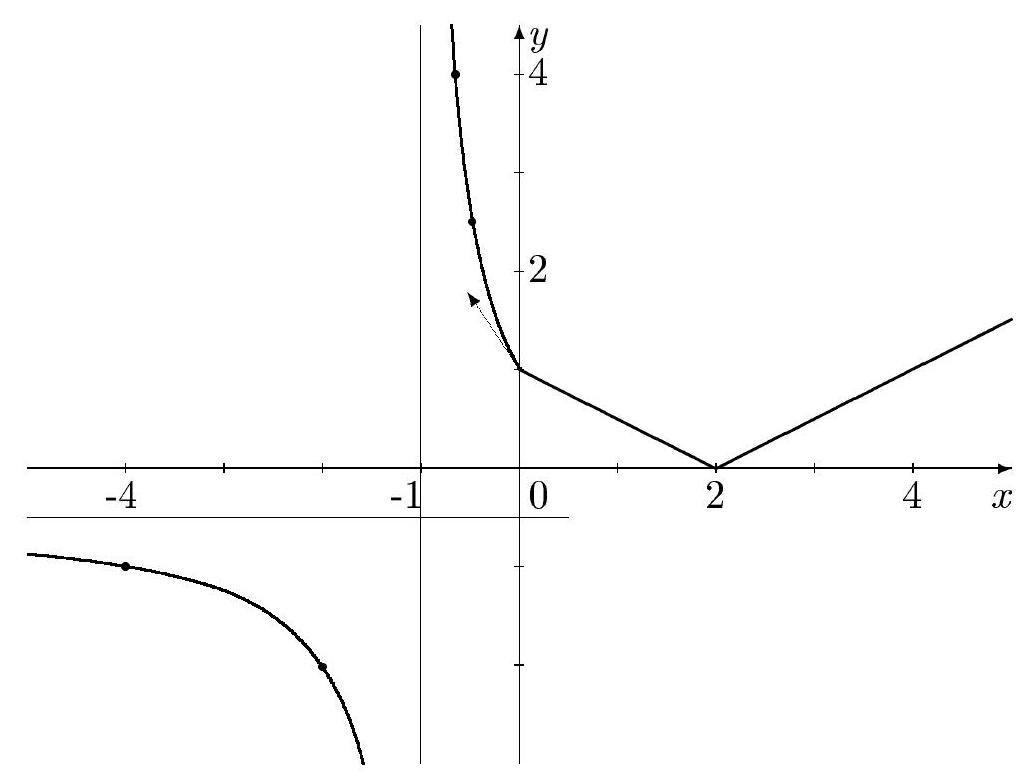
\includegraphics[max width=\textwidth, center]{2024_11_16_fe5b564401bf7db98894g-078}

Rys. 23\\
33.6. Asymptota pionowa obustronna $x=1$; asymptota pozioma lewostronna $y=-\frac{1}{2}$; asymptota ukośna prawostronna $y=\frac{1}{2} x-1$; minimum lokalne 0 dla $x=2$. Wykres funkcji przedstawiono na rysunku 23.\\
33.7. $\left[-\frac{5 \pi}{12}, \frac{\pi}{2}\right) \cup\left(\frac{\pi}{2}, \frac{11 \pi}{12}\right] \cup\{-\pi, \pi\}$.\\
33.8. Cosinus kąta rozwarcia wynosi $\frac{11}{13}$.\\
34.1. $3+\sqrt{5}$.\\
34.2. -4.\\
34.3. $-\frac{1}{2} x^{2}+x+2$ lub $-\frac{1}{18} x^{2}+\frac{1}{9} x-\frac{14}{9}$.\\
34.4. $\overrightarrow{A B}=[8,4], \overrightarrow{C D}=[-2,-1]$.\\
34.5. $\frac{6}{10}$.\\
34.6. Odległość $P$ od brzegu $\mathcal{F}$ wynosi $\frac{\sqrt{26}}{2}-2$. Zbiór $\mathcal{F}$ przedstawiono na rysunku 24.\\
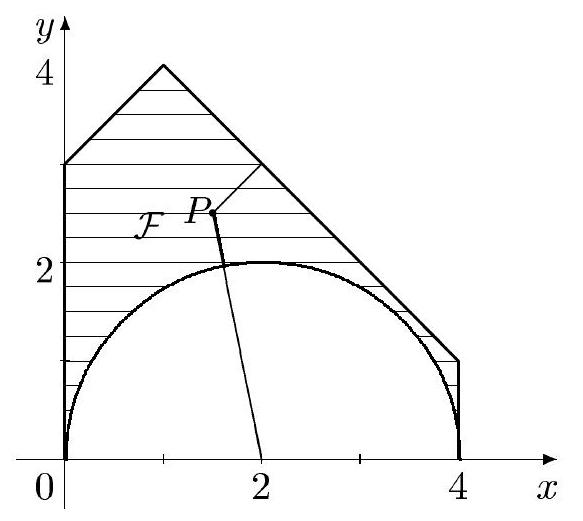
\includegraphics[max width=\textwidth, center]{2024_11_16_fe5b564401bf7db98894g-079}

Rys. 24\\
34.7. $f^{-1}(y)=-\frac{1}{1+2^{y}}, D_{f^{-1}}=\mathbf{R}, W_{f^{-1}}=(-1,0)$.\\
34.8. $\frac{1}{6} c^{3} \frac{1-3 \cos ^{2} \alpha}{\left(1+\cos ^{2} \alpha\right) \sin \alpha} \sqrt{\cos \alpha}$. Zadanie ma sens, gdy $\cos \alpha<\frac{\sqrt{3}}{3}$.\\
35.1. $4,-\frac{4}{3}, \frac{4}{9},-\frac{4}{27}, \ldots$\\
35.2. $\frac{2 \sqrt{3}-1}{5}$.\\
35.3. $\frac{a}{2}$.\\
35.5. $\frac{\pi}{4}+k \frac{\pi}{2}$ lub $\frac{\pi}{6}+k \pi \operatorname{lub} \frac{5 \pi}{6}+k \pi, \quad k \in \mathbf{Z}$.\\
35.6. $(x+4)^{2}+(y-1)^{2}=13$.\\
35.7. $\frac{2 r d^{3}}{4 r^{2}+d^{2}}$.\\
35.8. $m \in\left[-\frac{1}{2}, \frac{1}{2}\right) \cup\{1\}$.

Wskazówki do zadań

Uwaga. Podano wskazówki do wszystkich zadań. Zaproponowano pewną metodę rozwiązania każdego z zadań, najczęściej nie jedyną i z pewnością nie zawsze najprostszą.\\
1.1. Najpierw obliczyć oddzielnie masę stopu i masę srebra w stopie.\\
1.2. Pamiętać o wyznaczeniu dziedziny równania.\\
1.3. Oznaczyć nieznane współrzędne punktu $C$ przez $x$ i $y$, zapisać wektory $\overrightarrow{A C}$ i $\overrightarrow{B C}$ za pomoca $x$ i $y$ i korzystać z prostopadłości $\overrightarrow{A C} \perp \overrightarrow{B H}$ oraz $\overrightarrow{B C} \perp \overrightarrow{A H}$. Użyć iloczynu skalarnego.\\
1.4. Zamienić sinus na cosinus, stosując odpowiedni wzór redukcyjny i od razu przejść do porównywania kątów. Odpowiedź zapisać w postaci jednej serii rozwiązań.\\
1.5. Pamiętać, że $\log _{2} a^{2}=2 \log _{2}|a|$ i skorzystać z symetrii wykresu względem prostej $x=2$. Wykres otrzymać przez odbicia symetryczne i translacje standardowej krzywej $y=\log _{2} x$.\\
1.6. Najpierw rozważyć przypadek oczywisty $x<-6$. Dla $x>-6$ porównać odwrotności obu stron i przejść do nierówności kwadratowej. Pamiętać o dziedzinie nierówności.\\
1.7. Zastosować twierdzenie cosinusów. Podczas wykonywania rysunku pamiętać, że w rzucie równoległym zachowuje się równoległość oraz proporcje odcinków równoległych.\\
1.8. Proste równoległe mają takie same współczynniki kierunkowe. Współczynniki te wyznaczyć za pomoca pochodnych obu funkcji. Przy kreśleniu wykresu krzywej $y=\sqrt{1-x}$ zwrócić uwagę na lewostronne otoczenie punktu $x=1$.\\
2.1. Wystarczy pokazać, że dla każdego $n$ naturalnego wielomian $y^{2 n-1}+1$ jest podzielny przez dwumian $y+1$.\\
2.2. Kwadrat długości przekątnej wyrazić jako funkcję wysokości prostokąta wpisanego w trójkąt. Jest to funkcja kwadratowa i do jej badania nie jest potrzebna pochodna.\\
2.3. Przypadek $0<x<1$ jest oczywisty. Dla $x>1$ sprowadzić logarytmy do wspólnej podstawy 3 i przyjaćć $\log _{3} x=t$.\\
2.4. Warunek geometryczny zapisać w języku nierówności kwadratowej z parametrem.\\
2.5. Podstawić $x+5=t$ i badać równanie $||t|-1|=m$. Przypadki $m<0$ i $m=0$ rozpatrzeć bezpośrednio, a dla $m>0$ korzystać z tożsamości $(|a|=b) \Leftrightarrow(a=b$ lub $a=-b)$ prawdziwej dla $b \geq 0$.\\
2.6. Pomnożyć drugie równanie przez 2 i następnie odjąć oba równania stronami. Podstawienie $x-y=t$ prowadzi do równania kwadratowego z niewiadomą $t$.\\
2.7. Uzasadnić, że szukane punkty $A$ i $B$ leżą na osi $O x$ w odległości $5 \sqrt{2}$ od środka danego okręgu. Przy obliczaniu pola figury (która jest deltoid), najprościej jest korzystać z podobieństwa odpowiednich trzech trójkątów prostokątnych.\\
2.8. Dziedzinę równania określają warunek istnienia tangensa i warunek istnienia sumy nieskończonego ciągu geometrycznego. Korzystając ze wzoru $1+\operatorname{tg}^{2} \gamma=\frac{1}{\cos ^{2} \gamma}$ oraz ze wzorów podanych we wskazówkach do zad. 3.8 i 4.3, przekształcić obie strony do równości dwóch cosinusów lub sinusów i przejść od razu do porównywania kątów.\\
3.1. Podstawić $\sqrt{x}=t \mathrm{i}$ korzystać z własności funkcji kwdratowej oraz z monotoniczności pierwiastka kwadratowego.\\
3.2. Wyznaczyć środek $S$ rombu korzystając z relacji $S \in l$ oraz $\overrightarrow{A S} \perp l$ tzn. $\overrightarrow{A S}=a \vec{n}$, gdzie $\vec{n}=[2,1]$ jest wektorem prostopadtym do prostej $l$. Z warunku $\overrightarrow{A S} \perp \overrightarrow{S B}$ wynika, ze $\overrightarrow{S B}=-\overrightarrow{S D}=c[1,-2]$. Dane pole rombu pozwala wyznaczyć skalar $c$ i stąd od razu otrzymujemy współrzędne wierzchołków $B$ i $D$.\\
3.3. W dowodzie kroku indukcyjnego przeksztatcając lewą stronę doprowadzić do równości z prawa. Unikać dowodu metodą redukcji.\\
3.4. Pole podstawy obliczyć korzystajac z następujacego twierdzenia o zmianie pola figury płaskiej w rzucie prostokatnym:

Pole rzutu prostokatnego figury plaskiej jest równe polu tej figury pomnożonemu przez cosinus kata miedzy płaszczyznami figury i jej rzutu.\\
3.5. Kwadrat pola trójkąta wyrazić jako funkcję wysokości trójkąta. Funkcja ta jest wielomianem. Nie mylić tego zadania z zagadnieniem wyznaczania ekstremów lokalnych.\\
3.6. Zauważyć, że granica lewostronna pochodnej $y^{\prime}(x)$ w punkcie $x=\frac{5}{2}$ jest równa $-\infty$ co oznacza, że wykres jest w punkcie $\left(\frac{5}{2}, 0\right)$ styczny (lewostronnie) do prostej $x=\frac{5}{2}$.\\
3.7. Dla danych $r$ i $\alpha$ najmniejsze $d$ jest wtedy, gdy krótsza podstawa trapezu ma długość 0, tzn. trapez staje się trójkątem. Stąd otrzymać dziedzinę dla $d$. Analiza otrzymanych wzorów na pole i promień okręgu opisanego na trapezie prowadzi do błẹdnej dziedziny. W obliczeniach przyjąć jako niewiadomą połowę sumy obu podstaw i wyznaczyć ja z twierdzenia Pitagorasa w trójkącie zawierającym przekątną i wysokość trapezu. Promień okręgu opisanego wyznaczyć stosując twierdzenie sinusów.\\
3.8. Wyrażenie znajdujące się pod wartością bezwzględną przedstawić jako $a \cos (x-\alpha)$ dla odpowiedniego $\alpha \mathrm{i} a$, podnieść obie strony do kwadratu i skorzystać ze wzoru $2 \cos ^{2} \gamma=1+\cos 2 \gamma$.\\
4.1. Wyrazić $x$ przez niewiadomą liczbę składników $n$ i rozwiązać równanie kwadratowe z tą niewiadomą.\\
4.2. Zbudować model probabilistyczny doświadczenia, tj. określić zbiór $\Omega$ i prawdopodobieństwo $P$. Wygodniej jest obliczać prawdopodobieństwo zdarzenia przeciwnego, tj. że z wylosowanych cyfr nie można utworzyć liczby podzielnej przez 5.\\
4.3. Korzystać ze wzorów $1-\cos 2 \gamma=2 \sin ^{2} \gamma$ oraz $\sqrt{a^{2}}=|a|$. Obliczyć pochodne jednostronne bezpośrednio z definicji. Podczas rysowania wykresu zwrócić uwagę na otoczenie punktu $x=0$.\\
4.4. Korzystać z własności kạtów w równoległoboku. Następnie z przystawania odpowiednich (trzech) trójkątów wywnioskować, że przekątna utworzonego prostokąta jest równoległa do dłuższych boków równoległoboku.\\
4.5. Podczas rozwiązywania drugiej nierówności rozpatrzyć przypadki $y \in(0,1)$ oraz $y \in(1, \infty)$. Po podstawieniu $2^{x}=t$ przejść do nierówności kwadratowych zmiennej $t$. Nie zapomnieć o dziedzinie układu i szczegółowym ustaleniu, które punkty brzegu należą do rozważanego zbioru.\\
4.6. Korzystajac z własności okręgów stycznych zewnętrznie i wewnętrznie, wykazać, że suma odległości rozważanych punktów od środków obu danych okręgów jest stała i wynosi 12. Następnie zastosować geometryczna definicję elipsy.\\
4.7. Dziedzina funkcji jest określona przez warunki istnienia dwóch pierwiastków rzeczywistych równania (ale niekoniecznie różnych). Użyć wzorów Viète'a. Do różniczkowania przedstawić otrzymana funkcję jako sumę funkcji potęgowych. Ze względu na postać dziedziny nie można mówić o asymptocie ukośnej prawostronnej. Pamiętać, że ,,przyleganie" wykresu funkcji do asymptoty pionowej może być inne z każdej strony tej asymptoty.\\
4.8. Zauważyć, że czworościan ma płaszczyznę symetrii, która przechodzi przez wierzchołki $A, D$ i środek krawędzi $B C$. Środek kuli opisanej leży na tej płaszczyźnie w punkcie przecięcia się prostej prostopadłej do podstawy wystawionej w środku okregu opisanego na podstawie z symetralna krawędzi $A D$. Dziedzinę kąta $\alpha$ ustalić poprzez rozważania geometryczne (kąt $\alpha$ musi być większy od jego rzutu prostokątnego na podstawę).\\
5.1. Korzystać z tożsamości $(|a| \leq b) \Leftrightarrow(-b \leq a \leq b)$. Zbiór $A$ narysować za pomoca translacji standardowej krzywej $y=|x|$.\\
5.2. Wyznaczyć najpierw $\sin \alpha+\cos \alpha$ i stosować wzór na sumę sześcianów.\\
5.3. Rozważyć rodzinę prostych przechodzących przez punkt $P$. Proste te przecinając daną parabolę, wyznaczają cięciwy. Napisać układ równań, który spełniaja końce cięciw i nie rozwiązujac go, wyznaczyć środki\\
tych cięciw ze wzorów Viète'a. Zwrócić uwagę na dziedzinę (szukaną krzywą nie jest cała parabola!).\\
5.4. Wyznaczyć dziedzinę i podnieść obie strony równania do kwadratu, otrzymując proste równanie równoważne wyjściowemu.\\
5.5. Korzystajac ze schematu Bernoulliego, obliczyć odpowiednie prawdopodobieństwa dla obu strzelców. Dla drugiego strzelca najpierw obliczyć prawdopodobieństwo zdarzenia przeciwnego.\\
5.6. Jeśli $R$ jest niedużo większe niż $r$, to środki kulek leża na przekroju osiowym walca, gdyż kulki zajmują możliwie najniższe położenie. Największe $R$ (przy ustalonym $r$ ), przy którym kulki przyjmują takie położenie jest wtedy, gdy trzecia kulka (tj. leżąca najwyżej) będzie styczna z pierwszą (tj. leżącą na dnie naczynia). To odpowiada warunkowi $r<R \leq r+\frac{r \sqrt{3}}{2}$. Narysować przekrój osiowy walca, zaznaczając na nim przekroje kulek. Korzystać z twierdzenia o okręgach stycznych zewnętrznie i z twierdzenia Pitagorasa.\\
5.7. Przypadek $m=0$ rozpatrzeć oddzielnie. Dla $m \neq 0$ badać monotoniczność rozważając znak pochodnej. Prowadzi to do warunków, przy których odpowiedni trójmian kwadratowy w liczniku pochodnej jest nieujemny na R. Pamiętać, że funkcja jest rosnąca w pewnym przedziale także wtedy, gdy jej pochodna jest nieujemna i zeruje się w skończonej liczbie punktów.\\
5.8. Przekątne w rombie są równocześnie dwusiecznymi jego kątów. Jeśli więc dwa wektory są równej długości, to ich suma wyznacza kierunek dwusiecznej kąta między tymi wektorami.\\
6.1. Zauważyć, że $x=1$ spetnia równanie, a dla $x \neq 1$ przejść do porównania wykładników. Pamiętać o wyznaczeniu dziedziny równania.\\
6.2. Równanie stycznej do okręgu $\left(x-x_{0}\right)^{2}+\left(y-y_{0}\right)^{2}=r^{2} \mathrm{w}$ punkcie $A\left(x_{1}, y_{1}\right)$ leżącym na tym okręgu ma postać

$$
\left(x_{1}-x_{0}\right)\left(x-x_{0}\right)+\left(y_{1}-y_{0}\right)\left(y-y_{0}\right)=r^{2}
$$

6.3. Korzystać ze wzoru na sumę cosinusów oraz ze wzorów redukcyjnych. Przekształcać tylko lewa stronę i doprowadzić do równości z prawa.\\
6.4. Przyjąć, że iloraz $q$ ciagu jest większy od 1. Zauważyć, że środkowy wyraz ciagu jest równy 2 i ułożyć równanie z niewiadomą $q$.\\
6.5. Oznaczyć przez $A_{i}$ zdarzenie polegajace na wylosowaniu z pierwszej urny $i$ kul białych, $i=0,1,2,3$, i zastosować wzór na prawdopodobieństwo całkowite.\\
6.6. Zauważyć, że bryłę można podzielić na dwie (identyczne) połowy odpowiednią płaszczyzną prostopadłą do osi obrotu, a każda połowa składa się ze stożka oraz stożka ściętego o wspólnej podstawie.\\
6.7. Wyznaczyć tylko miejsca zerowe pochodnej i porównać wartości funkcji w tych punktach z jej wartościami na końcach przedziału. Nie tracić czasu na wyznaczanie ekstremów lokalnych.\\
6.8. Maksymalna wartość $k$ jest osiagana wtedy, gdy trójkąt jest równoramienny. Stąd ustalić dziedzinę $k$. Korzystać z podobieństwa odpowiednich trójkątów i z następujacej własności trójkąta prostokątnego:

Suma przyprostokatnych jest równa sumie średnic okregów wpisanego i opisanego.\\
7.1. Podstawić $3^{x}=t$ i korzystać z tożsamości podanej we wskazówce do zadania 5.1.\\
7.2. Wykorzystać zwiazzek współrzędnych punktu i jego obrazu w powinowactwie prostokątnym oraz związek pól figury i jej obrazu w tym przekształceniu.\\
7.3. Liczba $k$-elementowych podzbiorów zbioru $n$-elementowego wynosi $\binom{n}{k}$. Nie pominaćc zbioru pustego, który jest podzbiorem każdego zbioru.\\
7.4. Korzystać z twierdzenia o czworokącie opisanym na okręgu. Do wyznaczenia $\sin 15^{\circ}$ oraz $\cos 15^{\circ}$ nie korzystać z tablic, lecz przekształcić wyrażenie tak, aby otrzymać funkcje kąta $30^{\circ}$ (por. wskazówka do zad. 3.8).\\
7.5. Rozwiąań, dla których $x=y$, szukać także wśród nieskończenie wielu rozwiązań układu dla przypadku $m=3$.\\
7.6. Rozważyć oddzielnie przedziały $\left[-\frac{\pi}{2}, 0\right)$ oraz $\left[0, \frac{\pi}{2}\right]$, w których $\sin x$ ma stały znak, a funkcja cosinus jest monotoniczna. Zbiór rozwiązań zaznaczyć na wykresie jako podzbiór osi odciętych.\\
7.7. Korzystać z zależności między polami i objętościami figur i brył podobnych.\\
7.8. Skonstruować model probabilistyczny, czyli określić zbiór $\Omega$ oraz prawdopodobieństwo $P$. Oznaczyć przez $A_{\mathrm{I}}, A_{\mathrm{II}}$ zdarzenia polegajace na tym, że oba tomy odpowiednio I, II powieści znajdują się obok siebie i we właściwej kolejności. Interesuja nas zdarzenia $A_{\mathrm{I}} \cap A_{\mathrm{II}}$ oraz $A_{\mathrm{I}} \cup A_{\mathrm{II}}$. Prawdopodobieństwo tego drugiego obliczyć, stosując wzór na prawdopodobieństwo sumy dwóch dowolnych zdarzeń.\\
8.1. Pamiętać o warunku istnienia sumy nieskończonego ciagu geometrycznego.\\
8.2. Składnik $\binom{11}{i} 3^{i / 3} 2^{(11-i) / 2}$ będzie liczbac całkowita wtedy i tylko wtedy, gdy $i$ będzie podzielne przez 3, a $11-i$ będzie parzyste.\\
8.3. Korzystać z parzystości funkcji. Narysować w przedziale $[0, \infty)$ wykres funkcji $g(x)=x^{2}-2 x-3$ i zastosować geometryczną interpretację nałożenia na nią wartości bezwzględnej.\\
8.4. Najpierw określić dziedzinę nierówności. Napisać $x+1=\log _{2} 2^{x+1}$, podstawić $2^{x}=t$ i przejść do nierówności kwadratowej.\\
8.5. Do obliczenia objętości potrzebny jest tylko tangens kata nachylenia ściany bocznej do podstawy $t=\operatorname{tg} \alpha$. Warunek podany w zadaniu zapisać w postaci równania z niewiadomą $t$. Użyć tożsamości $\frac{1}{\cos ^{2} \alpha}=1+\operatorname{tg}^{2} \alpha$.\\
8.6. Kat prosty może się znajdować w jednym z trzech podanych wierzchołków trójkąta. Zastosować iloczyn skalarny.\\
8.7. Po wymnożeniu ,„na krzyż" skorzystać ze wzoru na iloczyn sinusów, doprowadzić do równości dwóch cosinusów i stąd od razu przejść do porównania kątów. Nie zapomnieć o uwzględnieniu dziedziny.\\
8.8. Korzystać z twierdzenia o stosunku pól figur podobnych. Zauważyć i uzasadnić, że suma skal podobieństwa trzech mniejszych trójkątów jest równa 1.\\
9.1. Pole powierzchni powiększonej kuli jest 1,44 razy większe od pola kuli wyjściowej.\\
9.2. Napisać równanie pęku prostych przechodzacych przez punkt $P$ i majacych ujemny współczynnik kierunkowy $m$ (dlaczego?). Wyznaczyć współrzędne punktów $A, B$ przecięcia się tych prostych z osiami układu oraz środków odcinków $A B$ w zależności od $m$. Eliminując parametr $m$ zapisać równanie krzywej w postaci $y=f(x)$.\\
9.3. Po podstawieniu $3^{x}=t$ zadanie sprowadza się do znalezienia warunków, przy których równanie kwadratowe z niewiadomą $t$ ma dwa różne pierwiastki dodatnie.\\
9.4. Rozważyć przekrój czworościanu płaszczyzną symetrii. Korzystając z podobieństwa odpowiednich dwóch trójkatów w tym przekroju, wykazać, że stosunek promieni kuli opisanej do wpisanej wynosi 3. Stąd obliczyć wysokość czworościanu, a następnie kolejno krawędź i objętość.\\
9.5. Dla $x<-3$ lewa strona jest dodatnia, a prawa ujemna i nierówność jest oczywiście spełniona. Dla $x>-3, x \neq 3$, obie strony sa dodatnie. Pomnożyć je przez $(x+3)|x-3|$. Po uproszczeniu dostajemy prosta nierówność, do której zastosować tożsamość $(|a| \leq b) \Leftrightarrow(-b \leq a \leq b)$.\\
9.6. Przyjacc $k \geq 1$ oraz oznaczyć przez $\alpha$ połowę większego z kątów ostrych trójkąta. Stosunek dwusiecznych wyrazić za pomocą $k$ oraz funkcji trygonometrycznych kąta $\alpha$ i przekształcić tak, aby wystapił tylko $\operatorname{tg} \alpha$. Wartość $\operatorname{tg} \alpha$ obliczyć, wiedząc, że $\operatorname{tg} 2 \alpha=k$.\\
9.7. Przedstawić funkcję w postaci $f(x)=1+\frac{4}{x-2}+\frac{8}{(x-2)^{2}}$ i w tej postaci ją różniczkować. Zauważyć, że wykres jest wyraźnie asymetryczny względem asymptoty $x=2$.\\
9.8. Napisać równanie stycznej w punkcie $\left(x_{0}, f\left(x_{0}\right)\right)$. Po podstawieniu do niego współrzędnych punktu $A$ otrzymujemy równanie trzeciego stopnia z niewiadomą $x_{0}$. Równanie to ma trzy pierwiastki wymierne. Przez bezpośrednie sprawdzenie wystarczy znaleźć dwa. Trzeci można obliczyć, wiedząc, że iloczyn pierwiastków wyraża się przez wyraz wolny i współczynnik przy najwyższej potędze $x_{0}$. Podczas rysowania wykresu korzystać z nieparzystości funkcji $f$ i już wyznaczonych stycznych. Dodatkowe badanie nie jest potrzebne.\\
10.1. Patrz wskazówka do zadania 3.3.\\
10.2. Kat widzenia odcinka $A B$ z punktu $C$ niewspółliniowego z $A$ i $B$ to kąt $\angle A C B$. Dany w zadaniu kąt zaznaczyć na przekroju osiowym stożka. Objętość wyrazić przez $l$ oraz funkcje trygonometryczne wielokrotności kąta $\alpha$. Uważnie stosować wzory redukcyjne i nie bać się napisać znaku minus we wzorze na objętość.\\
10.3. Patrz wskazówka do zad. 3.1.\\
10.4. Najpierw określić model probabilistyczny tj. $\Omega$ i $P$. Zdarzenie określone w treści zadania jest sumą czterech rozłacznych (dlaczego?) zdarzeń $A_{i}, i=1,2,3,4$, gdzie $A_{i}$ oznacza otrzymanie trzech kart w $i$-tym kolorze i jednej z innego koloru. $P\left(A_{i}\right)$ obliczyć bezpośrednio, korzystajac z tego, że $P$ jest prawdopodobieństwem klasycznym.\\
10.5. Wyznaczyć dziedzinę nierówności. Podstawić $\log _{2} x=t$ i korzystając z monotoniczności funkcji logarytmicznej o podstawie $\frac{1}{3}$, przejść do nierówności wymiernej.\\
10.6. Skorzystać ze wskazówki do zadania 6.2 i wyrazić współrzędne punktów styczności jako funkcje zmiennej $r$. Wygodniej jest szukać wartości największej kwadratu pola, który jest funkcja wymierną.\\
10.7. Korzystajac z tożsamości podanej we wskazówce do zadania 2.5 , wyznaczyć $y$ z drugiego równania, otrzymując dwa przypadki $y=\frac{3}{4} x$ oraz $y=\frac{3}{4} x-5$ i podstawić kolejno do pierwszego równania. Krzywa opisana pierwszym równaniem jest symetryczna względem osi rzędnych, a drugie równanie przedstawia dwie proste równoległe.\\
10.8. Przenieść wszystkie wyrazy na lewą stronę, użyć wzoru podanego we wskazówce do zadania 4.3, a następnie wzoru na sumę sinusów.\\
11.1. Jedną z figur jest trójkạt, którego pole stanowi ósmą część pola catego trójkąta (dlaczego?). Stąd wywnioskować, że $\alpha=\frac{\pi}{6}$.\\
11.2. Płaszczyzna przechodzaca przez jedną z krawędzi bocznych i środek kuli jest płaszczyzna symetrii i przecina podstawy graniastosłupa wzdłuż ich wysokości. Wybierając odpowiedni trójkąt, obliczyć szukaną wysokość. (Można też argumentować inaczej zauważajacc, że środek kuli opisanej oraz wierzchołki podstawy tworzą czworościan foremny, którego wysokość stanowi połowę szukanej wysokości graniastosłupa.)\\
11.3. Najpierw wyznaczyć ekstrema lokalne funkcji $g(x)=\frac{x}{1+x^{2}}$. Ponieważ $f(x)=a g(x)$, więc dobór $a$ jest natychmiastowy. Trzeba tylko pamiętać, że $a$ może być także ujemne i wtedy maksimum $f$ jest osiagane tam, gdzie $g$ ma minimum.\\
11.4. Wyznaczyć dziedzinę (warunek istnienia sumy nieskończonego ciagu geometrycznego) i pamiętać, że w niej mianownik sumy po lewej stronie jest dodatni. Pomnożyć obie strony przez ten mianownik i skorzystać ze wzoru podanego we wskazówce do zadania 3.8.\\
11.5. Użycie indukcji matematycznej nie jest potrzebne. Przekształcić prawạ stronę pisząc $2\binom{i}{2}=i(i-1)=i^{2}-i$ i pogrupować składniki kwadratowe oddzielnie, a liniowe zsumować jako kolejne liczby naturalne.\\
11.6. Oznaczyć środek jednego z rozważanych okręgów przez $A(x, y)$. Styczność do osi $O x$ oznacza, że promień tego okręgu wynosi $|y|$, czyli\\
odległość $A$ od środka $S$ danego okręgu wynosi $|A S|=2+|y|$ (styczność zewnętrzna!). Odległość $|A S|$ wyrazić bezpośrednio za pomoca $x$ i $y$ i tak otrzymać szukane równanie. Nazwać otrzymaną krzywą. Pamiętać, że środki okręgów leża na zewnątrz danego okręgu.\\
11.7. Przyjąć $\log _{3} m=t$ i korzystać ze wzorów Viète'a.\\
11.8. Najpierw wyznaczyć dziedzinę nierówności. Przypadek $x<0$ jest oczywisty, a dla $x>0$ można podnieść obie strony do kwadratu, następnie pomnożyć przez $x^{2}$, otrzymując nierówność kwadratową.\\
12.1. Narysować krzywe $y=\sqrt{x-3}$ oraz $y=4-x$ i za pomoca rysunku uzasadnić, że równanie to ma tylko jeden pierwiastek oraz że leży w przedziale $(3,4)$. Obliczyć go przez podniesienie obu stron równania do kwadratu.\\
12.2. Napisać rozkład $w(x)$ na czynniki i podstawić do obu stron równości $x=-1$.\\
12.3. Niech $A_{i}$ oznacza zdarzenie polegajace na wypadnięciu $i$ oczek na kostce. Wówczas $\Omega=A_{1} \cup \ldots \cup A_{6}$ i składniki sa parami rozłaczne. Zastosować wzór na prawdopodobieństwo całkowite. Dla wygody obliczyć najpierw prawdopodobieństwo zdarzenia przeciwnego do określonego w zadaniu, polegajacego na tym, że rzuty monetą nie dały żadnego orła.\\
12.4. Zauważyć, że są cztery takie okręgi; dwa w I ćwiartce i po jednym w II i IV ćwiartce. Srodek szukanego okregu ma w I ćwiartce postać $S(r, r)$, w II ćwiartce $S(-r, r)$, a w IV $S(r,-r)$, gdzie $r>0$ jest nieznanym promieniem rozważanego okręgu. W każdym przypadku niewiadomą $r$ wyznaczyć ze wzoru na odległość punktu od danej prostej, tj. $3 x+4 y=12$.\\
12.5. Poprowadzić wysokości sassiednich ścian bocznych do ich wspólnej krawędzi. Tworzą one wraz z przekątną podstawy trójkąt równoramienny, którego kąt przy wierzchołku wynosi $2 \alpha$ (z twierdzenia o trzech prostopadłych), a wysokość jest równa $d$.\\
12.6. Znając $P$ i $s$, obliczamy wysokość trapezu, a następnie jego przekątna z twierdzenia Pitagorasa, gdyż rzut prostokątny przekątnej na\\
podstawę ma długość $\frac{s}{2}$. Ramię trapezu wyznaczamy z podobieństwa odpowiednich trójkątów. Przekątna trapezu nie może przekroczyć średnicy okręgu. Stąd wynika warunek rozwiązalności zadania.\\
12.7. Dla $p=-1$ i $p=2$ układ jest nieoznaczony tzn. ma nieskończenie wiele rozwiązań. Rozwiązania te tworzą dwie proste. Dla każdego z pozostałych $p$ układ ma jedno rozwiązanie, które przy zmieniajacym się $p$ przebiega trzecią prostą. Na tych trzech prostych znaleźć punkty o podanej własności.\\
12.8. Badać kwadrat pola powierzchni jako funkcję $y$. Jest ona wielomianem. Nie mylić postawionego pytania z zagadnieniem wyznaczania ekstremów lokalnych. Wartość najmniejsza jest osiagana w punkcie $y=0$, a nie w minimum lokalnym. (Wynik ten kłóci się z intuicją, gdyż w tym przypadku tworząca stożka jest najdłuższa.)\\
13.1. Korzystając ze wzoru na cosinus różnicy kątów przedstawić lewa stronę w postaci $a \cos (x-\varphi)$ dla odpowiednio dobranego kąta $\varphi$.\\
13.2. Wektor $[12,5]$ jest wektorem normalnym prostej $l$, czyli wektor $\vec{v}=[5,-12]$ jest do niej równoległy (por. wskazówka do zadania 31.7.). Z definicji iloczynu skalarnego wynika, że liczba $\frac{|\overrightarrow{A B} \circ \vec{v}|}{|\vec{v}|}$ jest długością rzutu prostokątnego odcinka $A B$ na prostą $l$.\\
13.3. Wyznaczyć dziedzinę (nie zapomnieć o warunku $2^{m} \neq 7$ ) i użyć wzorów Viète'a. Wykres $f$ otrzymać ze standardowej krzywej $y=2^{m}$ przez translację i odbicie symetryczne.\\
13.4. Oznaczyć przez $B_{i}$ zdarzenie polegajace na tym, że pierwszy strzelec trafił $i$ razy, $i=0,1,2$, a przez $C_{j}$ zdarzenie, że drugi strzelec trafił $j$ razy, $j=0,1, \ldots, 5$. Wtedy rozważane zdarzenie ma postać $\left(B_{0} \cap C_{3}\right) \cup\left(B_{1} \cap C_{2}\right) \cup\left(B_{2} \cap C_{1}\right)$. Korzystać ze schematu Bernoulliego i niezależności par zdarzeń $B_{i}, C_{j}$.\\
13.5. Oddzielnie rozważyć $n$ parzyste i nieparzyste. Zapisać warunki na sumy wyrazów tego ciagu i eliminujac niewiadome wyrazić $a_{2}$ oraz $a_{3}$\\
tylko przez różnicę tego ciągu. Następnie obliczyć tę różnicę z równania $a_{2} a_{3}=48$ 。\\
13.6. Poprowadzić dwusieczną $A D$ i wyznaczyć $|B C|$, korzystajacc z podobieństwa trójkątów $A B C$ i $A D C$. Dalej korzystać z twierdzenia sinusów oraz ze wzoru na promień okręgu wpisanego w trójkat $r=\frac{S}{p}$.\\
13.7. Zbiór $A$ wyznaczyć korzystając ze wskazówki do zadania 5.1. Uzasadnić (podnoszac obie strony do kwadratu), że krzywa o równaniu $y=\sqrt{4 x-x^{2}}$ nie jest łukiem paraboli lecz półokręgiem. Obliczyć odległość punktu $P$ od każdej z trzech części brzegu zbioru $A \cap B$ i porównać je.\\
13.8. Korzystać z parzystości funkcji. Z postaci dziedziny wynika, że funkcja nie może mieć asymptot (dlaczego?). Granica lewostronna pochodnej w punkcie $x=\sqrt{8}$ wynosi $-\infty$, więc prosta $x=\sqrt{8}$ jest styczna do wykresu funkcji $f(x)$. Dla sporzadzenia wykresu dobrać odpowiednia jednostkę na obu osiach układu współrzędnych.\\
14.1. Korzystać ze wskazówki do zad. 7.3. Otrzymane wyrażenie jest ciagiem rosnącym i zadanie może mieć co najwyżej jedno rozwiązanie.\\
14.2. Uzasadnić, że promienie kolejnych okręgów tworzą ciagg geometryczny, którego iloraz jest równy pierwszemu wyrazowi ciagu.\\
14.3. Korzystać z rachunku wektorowego i iloczynu skalarnego. Zauważyć, że wszystkie proste z danej rodziny przechodzą przez punkt $P(1,1)$.\\
14.4. Stosować wzór na tangens różnicy kątów. Wyznaczyć dziedzinę tej tożsamości i funkcji $f(x)$.\\
14.5. Skorzystać ze wskazówki do zadania 7.2. Rozważana figura jest różnicą odcinka danego koła, wyznaczonego przez oś odciętych, oraz jego obrazu w powinowactwie określonym w zadaniu.\\
14.6. Zastosować podana nierówność i sprowadzić logarytmy do podstawy 2. Następnie wykazać, że iloraz rozważanego ciagu geometrycznego jest większy od 1 i stąd od razu otrzymać odpowiedź.\\
14.7. Patrz wskazówka do zadania 7.8.\\
14.8. Rozważyć przekrój płaszczyzną przechodzącą przez przekątna podstawy i wierzchołek ostrostupa. Z twierdzenia o odcinkach stycznych do kuli poprowadzonych z ustalonego punktu wynika, że punkt styczności kuli z krawędzią boczna leży w odległości $\frac{a}{2}$ od wierzchołka podstawy. Korzystajac z tej obserwacji obliczyć krawędź boczną na dwa sposoby i stąd wyznaczyć promień kuli.\\
15.1. Oznaczyć przez $x$ odległość miejscowości, a przez $y$ prędkość drugiego rowerzysty. Ułożyć układ dwóch równań z tymi niewiadomymi, zapisując informacje podane w treści zadania.\\
15.2. Określić dziedzinę nierówności. Przypadek $x<0$ jest oczywisty. Dla $x>0$ podnieść obie strony do kwadratu, po pomnożeniu przez $x^{2}$ otrzymujemy nierówność dwukwadratowa.\\
15.3. Pole powierzchni dachu obliczyć z twierdzenia podanego we wskazówce do zadania 3.4. Objętość dachu obliczyć, dzieląc bryłę płaszczyznami pionowymi na dwa ostrostupy i graniastostup.\\
15.4. Wyrazić $w_{n+1}$ przez $w_{n}$, korzystając z danych zadania. Uzasadnić, że ciag $\Delta_{n}=w_{n+1}-w_{n}$ jest ciagiem geometrycznym o ilorazie 1,015 oraz że $w_{n}=w_{1}+\Delta_{1}+\ldots+\Delta_{n-1}$. Pensja w kwietniu 2002 roku jest równa $w_{6}$.\\
15.5. Funkcja $f(x)$ jest rosnąca i zbiorem jej wartości jest R. Stąd $f^{-1}(x)=\sqrt[3]{x}$ jest określona na $\mathbf{R}$, a jej wykres jest odbiciem symetrycznym wykresu $f(x)$ względem prostej o równaniu $y=x$. Wykres funkcji $h(x)$ w przedziale $(0, \infty)$ otrzymać przez translację części wykresu funkcji $f^{-1}(x)$ i korzystajac z parzystości funkcji $h(x)$.\\
15.6. Wyznaczyć dziedzinę, pomnożyć obie strony przez mianownik, przejść za pomocą wzoru redukcyjnego do równości dwóch cosinusów i stąd od razu do porównania katów. Wynik zapisać w postaci jednej serii.\\
15.7. Patrz wskazówka do zadania 5.8.\\
15.8. Wyznaczyć dziedzinę funkcji; nie pominać punktu $x=0$. Sumę wyrazów nieskończonego ciagu geometrycznego zapisać w postaci $f(x)=x+1+\frac{2}{x-2}, \mathrm{z}$ której od razu odczytać równania asymptot (uważać na dziedzinę). Ta postać jest także wygodna do różniczkowania (nie jest celowe stosowanie wzoru na pochodna ilorazu). Podczas rysowania wykresu jeszcze raz uważać na dziedzinę.\\
16.1. Oznaczyć przez $x, y, z$ ceny odpowiednio początkową, po obniżce i po podwyżce. Wyrazić $y$ przez $x$ oraz $z$ przez $y$ i w konsekwencji $z$ przez $x$.\\
16.2. Punkt $(0,0)$ rozpatrzyć oddzielnie. Zauważyć, że zbiór jest symetryczny względem obu osi układu współrzędnych i wyznaczyć (oraz opisać) najpierw tę część, która leży w I ćwiartce.\\
16.3. Wysokości ścian bocznych oraz odcinek łączący środki dwóch odpowiadających im krawędzi podstawy tworzą trójkąt równoramienny o kacie przy wierzchołku $2 \alpha$ i podstawie $\frac{a}{2}$ (dlaczego?). Podstawa tego trójkata nie przechodzi przez spodek wysokości ostrosłupa. Przez porównanie tego trójkatata z jego rzutem prostokątnym na podstawę ostrosłupa, określić dziedzinę dla kąta $\alpha$.\\
16.4. Można odciąć narożniki zawierajace wierzchołki kątów ostrych równoległoboku lub zawierające wierzchołki kạtów rozwartych. Należy wybrać (i uzasadnić odpowiednim rachunkiem) to cięcie, które daje romb o większym polu, tj. odciąć narożniki zawierające kąty rozwarte. Punkt, przez który należy poprowadzić cięcie wyznaczyć z twierdzenia cosinusów.\\
16.5. $\sqrt{2}$ zamienić na potęgę o podstawie 2 i wykładniku ułamkowym, skorzystać z reguł działań na potęgach, przejść do porównania wykładników i podstawić $\log _{2} x=t$.\\
16.6. Wyrażenie w mianowniku zapisać w postaci $3+a \cos (x-\alpha)$ (por. wskazówka do zadania 3.8). Wykazać, że $|a|<3$, co oznacza, że dziedzina funkcji $f(x)$ jest $\mathbf{R}$, a mianownik jest dodatni w $\mathbf{R}$. Wartość najmniejsza funkcji $f(x)$ jest osiagana w tym punkcie, w którym mianownik jest największy i na odwrót. Użycie pochodnej jest zbędne.\\
16.7. Oddzielnie rozpatrzyć przypadek $p=0$. Dla $p \neq 0$ równanie dwukwadratowe ma dokładnie dwa różne pierwiastki, gdy odpowiadające mu równanie kwadratowe ma wyróżnik równy zeru bądź ma wyróżnik dodatni i jednocześnie jeden z pierwiastków ujemny.\\
16.8. Napisać równanie stycznej w punkcie $A$, korzystając z pochodnej funkcji. Styczna ta przecina wykres funkcji w innym punkcie $B$. Przy wyznaczaniu tego punktu otrzymujemy równanie trzeciego stopnia, które ze względu na styczność w punkcie $A$ ma pierwiastek podwójny 3 i tylko trzeba znaleźć trzeci pierwiastek (por. wskazówka do zad. 9.8).\\
17.1. Najpierw rozważyć przypadek, gdy iloraz równy zeru, tzn. $\cos x=0$. Wtedy wszystkie dalsze wyrazy ciągu są równe zeru. Jeśli $\cos x \neq 0$, to liczby $\sin x, \cos x, \sin 2 x$ tworza ciag geometryczny wtedy i tylko wtedy, gdy kwadrat liczby środkowej jest iloczynem liczb skrajnych, tzn. gdy $\cos x=2 \sin ^{2} x$. Podstawić $\cos x=t$.\\
17.2. Losowe dzielenie drużyn na grupy interpretować jako permutacje numerów wszystkich drużyn, tj. liczb $1,2, \ldots, 16$, gdzie kolejne czwórki wyrazów permutacji wyznaczaja skład kolejnych grup. Pamiętać o określeniu na poczatku modelu probabilistycznego, tj. $\Omega$ i $P$.\\
17.3. Zauważyć, że dane wyrażenie można zapisać w postaci $\left[\left(x^{2}+x+1\right)^{3}+x^{3}\right]-\left[x^{6}+2 x^{3}+1\right]$ i stosując wzór na sumę sześcianów, wykazać, że oba składniki tej sumy dzielą się przez $(x+1)^{2}$.\\
17.4. Z symetrii figury wynika, że środek $S$ okręgu stycznego w dwóch punktach do danej paraboli leży na osi rzędnych, tzn. mamy $S\left(0, y_{0}\right)$, przy czym $y_{0}>r$. Styczność oznacza, że równanie kwadratowe z niewiadomą rzędna $y$ punktu styczności powinno mieć dodatni pierwiastek podwójny, co jest spełnione, gdy wyróżnik tego równania jest równy zeru, a współczynnik przy niewiadomej $y$ jest ujemny.\\
17.5. Dbać o logiczna poprawność zapisu całego dowodu indukcyjnego. W dowodzie kroku indukcyjnego przekształcać tylko lewą stronę, pamiętając, że zwiększenie $n$ o 1 powoduje pojawienie się dwóch dodatkowych składników.\\
17.6. Ustalić dziedzinę nierówności i korzystać z własności logarytmu o podstawie mniejszej od 1 (dziedzina jest zawarta w odcinku $(0,1)$ ).\\
17.7. Uzasadnić, że $\angle A S D$ jest prosty. To oznacza, że dane $c=|A D|$ oraz $d=|A S|, \quad d \sqrt{2} \geq c>d$, jednoznacznie określaja trójkąt $A S D$ oraz promień okręgu $r$ i kat $\angle D A B$ trapezu. Wyznaczyć $r$ oraz długości odcinków, na które punkt styczności dzieli $A D$. Możliwe sa dwa przypadki: albo podział $A B$, liczac od wierzchołka $A$, jest w stosunku 2:1, albo w stosunku 1:2. W drugim przypadku może się zdarzyć, że kąt przy wierzchołku $B$ jest rozwarty.\\
17.8. Możliwe są dwa przypadki: albo w jednym z wierzchołków podstawy wszystkie katy płaskie kąta trójściennego wychodzacego z tego wierzchołka są ostre, albo wszystkie sa rozwarte. W obu przypadkach poprowadzić płaszczyznę symetrii przez ten wierzchołek i przeciwległy wierzchołek drugiej podstawy oraz przez odpowiednie przekatne obu podstaw. Nieznaną wysokość równoległościanu obliczamy z twierdzenia o trzech prostopadłych. Obliczamy najpierw wysokość rombu tworzacego każdą ścianę równoległościanu, następnie odległość spodka wysokości równoległościanu od krawędzi podstawy i wreszcie z twierdzenia Pitagorasa wysokość równoległościanu. W obu przypadkach obliczenia sa analogiczne.\\
18.1. Zarówno licznik jak i mianownik są sumami skończenie wielu (ustalić ilu) wyrazów dwóch ciagów geometrycznych. Obliczyć te sumy i podzielić licznik i mianownik przez $2^{2 n}$.\\
18.2. Szukana prosta przechodzi przez środek odcinka $A B$ i jest prostopadła do danej prostej. Stąd od razu można napisać równanie tej prostej.\\
18.3. Patrz wskazówka do zadania 10.2.\\
18.4. Oznaczyć przez $x, y$ ceny długopisu i zeszytu. Wtedy $x>y \geq 0,50$. Ułożyć układ dwóch równań z niewiadomymi $x, y$ i parametrem $k$. Oddzielnie rozważyć przypadek $k=2$, dla którego układ jest nieoznaczony, oraz $k \neq 2$, gdy układ ma jedno rozwiązanie. W pierwszym przypadku wybrać wszystkie $k$, dla których $x$ i $y$ wyrażają się w pełnych dziesiątkach groszy i spełniaja warunek $x>y \geq 0,50$. Odpowiedni rysunek ułatwia znalezienie wszystkich rozwiązań.\\
18.5. Korzystać ze wzoru $\sin 2 \gamma=\frac{2 \operatorname{tg} \gamma}{1+\operatorname{tg}^{2} \gamma}$ i podstawić $\operatorname{tg} \gamma=t$.\\
18.6. Stosować schemat Bernoulliego. Drugie pytanie dotyczy prawdopodobieństwa warunkowego rozważanego zdarzenia przy warunku, że co najmniej jedna żarówka jest dobra.\\
18.7. Ponieważ promień szukanego okręgu jest bardzo mały, należy przyjaćć na rysunku duża jednostkę i narysować tylko odpowiedni łuk danego okręgu. W obliczeniach korzystać z twierdzenia o okręgach stycznych zewnętrznie oraz z twierdzenia Pitagorasa w trójkaçie, którego wierzchołkami są środki obu okręgów oraz rzut prostokątny środka małego okręgu na odcinek $A S$.\\
18.8. Pole i objętość ostrosłupa ściętego wyrazić jako funkcje długości $x$ krawędzi górnej podstawy tego ostrosłupa, $0<x<1$. Korzystać z twierdzenia o stosunku pól i objętości figur i brył podobnych. Wyznaczyć miejsce zerowe pochodnej znalezionej funkcji, zbadać znak pochodnej i uzasadnić, że w tym punkcie funkcja osiaga nie tylko ekstremum lokalne, ale także wartość największą.\\
19.1. Wektory $\overrightarrow{B M}$ oraz $\overrightarrow{B K}$ wyrazić za pomoca wektorów $\overrightarrow{A B}, \overrightarrow{B C}$ oraz $\overrightarrow{C D}$. Mając współrzędne tych wektorów, od razu obliczyć pole $\triangle K M B$.\\
19.2. Napisać związek przekątnej prostopadłościanu z długościami jego krawędzi i stąd obliczyć nieznaną różnicę ciągu. Odrzucić to rozwiązanie, które prowadzi do ujemnych długości krawędzi.\\
19.3. Zbiór $A$ wyznaczyć korzystajac ze wskazówki do zadania 13.7 (w części dotyczącej zbioru $B$ w tamtej wskazówce). Dobrać $s$ tak, aby prosta $B_{s}$ miała jeden punkt wspólny ze zbiorem $A$ (co to znaczy geometrycznie?) i stąd od razu podać odpowiedź.\\
19.4. Korzystając z nierówności trójkạta, ustalić, które pary odcinków mogą być podstawami trapezu. Są trzy takie możliwości (spośród sześciu). W dwóch przypadkach pole trapezu jest mniejsze od 11 arów. Wykazać to, zauważając, że wysokość trapezu jest mniejsza od każdego z jego ramion. W trzecim przypadku należy obliczyć pole i wykazać, że przekracza ono 11 arów.\\
19.5. Ustalić dziedzinę dla parametru $m$ i stosować wzory Viète'a. Za pomoca pochodnej wykazać, że kwadrat różnicy pierwiastków, jako funkcja zmiennej $m$, jest malejący w wyznaczonej dziedzinie.\\
19.6. W dowodzie kroku indukcyjnego uważnie stosować reguły działań na potęgach.\\
19.7. Sumy z lewych stron przekształcić na iloczyny. Stąd wywnioskować, że $\sin (x+y)=1$, czyli z drugiego równania $\cos (x-y)=\frac{1}{2}$ i od razu przejść do układów równań liniowych z niewiadomymi $x$ i $y$.\\
19.8. Oznaczyć $|C D|=|C A|=|C B|=a$. Ponieważ $C D \perp A D$ oraz $C D \perp B D$, więc dwie ściany boczne sa prostopadłe do podstawy $A B D$ (będącej trójkątem równobocznym) i tworza ze sobą kąt $60^{\circ}$. Kat między podstawą i płaszczyzna $A B C$ wyznaczamy, przecinając czworościan płaszczyzną symetrii $C D E$, gdzie $E$ jest środkiem $A B$. Dla wyznaczenia kąta między płaszczyzną $A B C$ i płaszczyzną $B C D$ (i równocześnie $A C D$ ) należy z wierzchołka $D$ poprowadzić wysokość czworościanu na ścianę $A B C$. Ponieważ $\triangle B C D$ jest prostokątny i równoramienny, więc z twierdzenia o trzech prostopadłych wynika, że spodek tej wysokości leży w środku okręgu opisanego na trójkacie $A B C$. Wyrazić tę wysokość przez $a$, obliczając objętość czworościanu na dwa sposoby i stąd od razu wyznaczyć sinus rozważanego kąta.\\
20.1. Oddzielnie rozpatrzeć $m=0$ i $m=2$. Dla pozostałych parametrów $m$ korzystać z faktu, że oś symetrii paraboli przechodzi przez jej wierzchołek.\\
20.2. Uzasadnić, że środek danej kuli i środek kuli wpisanej w dana bryłę tworzą przekątną sześcianu o krawędzi równej promieniowi kuli wpisanej. Rozważyć przekrój płaszczyzną symetrii zawierającą środki obu kul.\\
20.3. Określić model probabilistyczny, tj. $\Omega$ i $P$. Obliczyć prawdopodobieństwo zdarzenia przeciwnego, korzystajac ze wzoru na prawdopodobieństwo sumy dwóch dowolnych zdarzeń.\\
20.4. Stosować wzór na odległość punktu od prostej. Pamiętać, że rozważamy tylko punkty wewnątrz danego trójkąta. Nazwać wyznaczona krzywá.\\
20.5. Rozważyć przypadki $x>1$ i $x<1$ i uprościć wzór określający funkcję. Podczas rysowania wykresu pamiętać o dziedzinie funkcji.\\
20.6. Napisać $\frac{1}{x^{2}}=|x|^{-2}$ i rozważyć przypadki $|x|=1, \quad|x|<1$ oraz $|x|>1$. Nie stosować bezpośrednio definicji wartości bezwzględnej.\\
20.7. Warunek zadania oznacza, że rozważane styczne mają współczynniki kierunkowe +1 lub -1 . Obliczyć pochodną funkcji $f$, przyrównać jej wartość bezwzględną do 1 i rozwiązać otrzymane równanie niewymierne.\\
20.8. Oznaczyć $x=|A D|$ oraz $y=|A E|$. Ze stosunku pól obliczyć $x y$, a z twierdzenia sinusów w trójkaçie $A D E$ iloraz $\frac{x}{y}$. Nie wyznaczać jawnie $x$ i $y$, lecz tylko sumę $x+y$ (korzystać ze wzoru skróconego mnożenia).\\
21.1. Oznaczyć przez $x, y$ krawędzie mniejszych sześcianów. Napisać układ równań z niewiadomymi $x$ i $y$ i nie wyznaczając ich jawnie, obliczyć tylko $x^{2}+y^{2}$ za pomoca wzorów skróconego mnożenia. Stąd od razu otrzymać odpowiedź.\\
21.2. Wyznaczyć wektory $\overrightarrow{A C}$ i $\overrightarrow{B D}$ i zastosować iloczyn skalarny oraz tożsamość podana we wskazówce do zad. 2.8.\\
21.3. Wyznaczyć skalę podobieństwa trójkatón i wyrazić przeciwprostokątna przez promień okręgu $r$. Stąd obliczyć sumę przyprostokątnych wyjściowego trójkąta i w konsekwencji sumę cosinusów kątów ostrych trójkąta. Podnosząc tę równość do kwadratu obliczyć oba cosinusy.\\
21.4. Przenieść niewymierność do mianownika i podzielić licznik i mianownik przez $n$. Korzystać z faktu, że złożenie funkcji malejących jest funkcją rosnacaca.\\
21.5. Korzystać ze wzoru podanego we wskazówce do zadania 3.8.\\
21.6. Napisać warunki określajace dziedzinę, ale nie wyznaczać dziedziny w sposób jawny. Sprowadzić logarytmy do wspólnej podstawy 4 i przejść do równania algebraicznego trzeciego stopnia. Obliczyć jego pierwiastki i wybrać te, które należą do dziedziny.\\
21.7. Narysować przekrój osiowy stożka. Objętość wyrazić jako funkcję wysokości stożka. Nie mylić tego zadania z zagadnieniem wyznaczania ekstremów lokalnych.\\
21.8. Obie parabole łacznie ze stycznymi tworzą figurę mającą środek symetrii $S$ (dlaczego?). Więc szukane styczne przechodza przez punkt $S$. Wyznaczyć $S$. Napisać równanie pęku prostych przechodzacych przez $S$ i z warunku styczności (wyróżnik odpowiedniego równania kwadratowego równy zeru) obliczyć współczynniki kierunkowe szukanych stycznych.\\
22.1. Wykorzystać parzystość funkcji. Podczas rysowania wykresu zwrócić uwagę na otoczenie punktu $x=0$.\\
22.2. Uzasadnić, że liczby metrów sześciennych wody wpływające do basenu w kolejnych minutach tworza ciag arytmetyczny. We wszystkich obliczeniach przyjać minute jako jednostkę czasu. Dane liczbowe podstawić na końcu.\\
22.3. Oznaczyć średnice obu podstaw przez $x$ i $y$. Ułożyć układ równań $z$ niewiadomymi $x, y$ i przejść od razu do alternatywy układów równań liniowych.\\
22.4. Z twierdzenia sinusów wynika, że znany jest także bok $|B C|$. W okręgu o promieniu $R$ zaznaczyć cięciwę o długości $|B C|$ i rozważać kạty wpisane oparte na łuku wyznaczonym przez tę cięciwę. Wybrać takie położenie (położenia) wierzchołka $A$, które daje $|A B|=\frac{8}{5} R$. W zależności od wielkości kąta $\alpha$ (czyli długości cięciwy $|B C|$ ) mamy różne przypadki, które należy kolejno rozpatrzyć.\\
22.5. Od razu zlogarytmować obie strony, przyjmujac za podstawe logarytmu liczbę 8.\\
22.6. Wyrazić wektory $\overrightarrow{C B}$ i $\overrightarrow{C D}$ przez $\overrightarrow{A B}=\vec{u}$ i $\overrightarrow{B D}=\vec{v}$ i użyć iloczynu skalarnego.\\
22.7. Wyznaczyć dziedzinę równania. Pomnożyć obie strony przez wyrażenie $(\sin x \cos x)$ i doprowadzić do równania elementarnego postaci $\sin (f(x))=\sin (g(x))$. Rozwiązania zapisać w postaci jednej serii.\\
22.8. Napisać równanie stycznej w punkcie $x_{0}$, wyznaczyć punkty przecięć tej stycznej z osiami układu współrzędnych i wyrazić kwadrat długości odcinka stycznej jako funkcję $x_{0}$. Do różniczkowania pozostawić tę funkcję w postaci sumy funkcji potegowych. Nie mylić postawionego pytania z zagadnieniem wyznaczania ekstremów lokalnych.\\
23.1. Liczba ,stów" utworzonych z danych liter odpowiada liczbie permutacji z powtórzeniami.\\
23.2. Zadanie rozwiązać bez dzielenia wielomianów. Zauważyć, że iloraz danych wielomianów ma postać $x+a$ i wyznaczyć najpierw niewiadomą $a$.\\
23.3. Wykorzystać symetrię figury i twierdzenie o okręgach wzajemnie stycznych.\\
23.4. Przez punkty $K$ i $L$ poprowadzić płaszczyzny prostopadłe do płaszczyzny podstawy i równoległe do $B C$. Obliczać oddzielnie objętości każdej z tak otrzymanych brył (dwie z nich są identyczne). Por. zad. 15.3.\\
23.5. Wyznaczyć dziedzinę nierówności. Rozpatrzyć najpierw oczywisty przypadek $x<0$. Dla $x>0$ podnieść obie strony nierówności do kwadratu i rozwiązać nierówność dwukwadratowa. Wykresem funkcji z prawej strony nierówności nie jest łuk paraboli lecz inna dobrze znana krzywa (por. wskazówka do zad. 13.7).\\
23.6. Dowód kroku indukcyjnego przeprowadzić wprost. Nie stosować niewygodnej metody redukcji. Dbać o logiczna poprawność zapisu dowodu.\\
23.7. Punkt $M\left(y_{0}^{2}, y_{0}\right), y_{0}>0$, leży najbliżej $P$, gdy odcinek $P M$ jest prostopadły do stycznej do danej krzywej w punkcie $M$. Użyć rachunku wektorowego.\\
23.8. Ponieważ współczynnik przy $x^{2}$ jest dodatni, więc pierwiastki trójmianu kwadratowego będą leżeć w odcinku $(0,1)$, gdy odcięta wierzchołka paraboli będącej jego wykresem znajdzie się w tym przedziale, a wartości trójmianu dla $x=0$ i $x=1$ będą dodatnie. Otrzymane nierówności trygonometryczne rozwiązać analitycznie. Ewentualny rysunek służy do ilustracji rozwiązania.\\
24.1. Pamiętać o warunku istnienia sumy nieskończonego ciagu geometrycznego.\\
24.2. Zaczać od określenia modelu probabilistycznego, tj. zbioru zdarzeń elementarnych $\Omega$ oraz prawdopodobieństwa $P$. Oznaczyć przez $A$ zdarzenie polegajace na tym, że kości pasują do siebie, a przez $A_{i}$ zdarzenie, że na jednym z pól obu kości jest $i$ oczek, a na pozostałych polach cokolwiek, $i=0, \ldots, 6$. Wtedy $A=A_{0} \cup \ldots \cup A_{6}$ i składniki parami wykluczaja się (dlaczego?). Obliczyć $P\left(A_{i}\right)$ i skorzystać z własności prawdopodobieństwa.\\
24.3. Wykazać, że dla $m=10$ układ jest sprzeczny, a dla $m \neq 10 \mathrm{ma}$ jedno rozwiązanie. Zauważyć, że dla żadnego $m \in \mathbf{R}$ para $(1,1)$ nie jest rozwiązaniem układu.\\
24.4. Określić dziedzinę dla kąta $\alpha$ porównując ten kąt z jego rzutem prostokatnym na podstawę. Z twierdzenia o trzech prostopadłych uzasadnić, że $A B \perp B D^{\prime}$. Wywnioskować stąd, że kąt $D B D^{\prime}$ jest kątem płaskim kąta dwuściennego między płaszczyzną $A B D^{\prime} E^{\prime}$ i podstawa graniastosłupa.\\
24.5. Rozważyć przypadki $x<1$ oraz $x>1$ i pomnożyć obie strony przez mianownik (dodatni lub ujemny, odpowiednio). Jedna z nierówności podwójnych jest automatycznie spełniona, a druga, przez podstawienie $2^{x}=t$, sprowadza się do do nierówności kwadratowej. Nie potrzeba rozważać nierówności wyższego stopnia.\\
24.6. Zauważyć, że $\operatorname{tg} 82^{\circ} 30^{\prime}=\frac{1}{\operatorname{tg} 7^{\circ} 30^{\prime}}$ oraz że $82^{\circ} 30^{\prime}-7^{\circ} 30^{\prime}=75^{\circ}$ i zastosować wzór na tangens różnicy kątów. Następnie korzystać z równości $75^{\circ}=45^{\circ}+30^{\circ}$.\\
24.7. Skorzystać ze wskazówki do zadania 6.2 , a w drugiej części rozwiązania ze wskazówki do zad. 5.8.\\
24.8. Przypadek $a=1$ wymaga oddzielnego rozpatrzenia (dlaczego?). Pochodna funkcji $\frac{b}{x^{2}-1}=b\left(x^{2}-1\right)^{-1}$ wygodniej jest obliczać za pomoca reguły różniczkowania funkcji złożonej. Zauważyć, że dla $a=3, b=32$, gwarantujących ciagłość i różniczkowalność $f(x)$, punkt $P(3,4)$ jest jej punktem przegięcia.\\
25.1. Najpierw rozpatrzyć oczywisty przypadek $t=0$, a następnie $t \neq 0$.\\
25.2. Korzystając z twierdzenia Talesa wykazać, że przekrój jest równoległobokiem. Następnie prowadzić płaszczyznę symetrii czworościanu i stosujac twierdzenie o trzech prostopadłych, wykazać, że przekrój jest prostokatem.\\
25.3. Określić dziedzinę nierówności. Zauważyć, że szukany zbiór jest symetryczny względem początku układu, co pozwala ograniczyć rozważania do I ćwiartki układu. Rozpatrzyć przypadki $x y>1$ oraz $x y<1$.\\
25.4. Półprosta wychodząca ze środka okręgu i zawierajaca dany punkt $A$ przecina ten okrąg w punkcie $A^{\prime}$ leżaccym najbliżej punktu $A$. Stąd $\left|A A^{\prime}\right|$ jest odległościa punktu $A$ od danego okręgu. Prowadząc rozważania geometryczne uzasadnić, że dla punktów leżących wewnątrz okręgu zachodzi relacja $O A+P A=10$, co oznacza, że $A$ leży na elipsie o ogniskach $O$ i $P$ (por. wskazówka do zad. 4.6). Inaczej jest, gdy $A$ leży na zewnątrz danego okręgu.\\
25.5. Wszystkie przeprowadzane losowania są wzajemnie niezależne, więc ich kolejność nie ma wpływu na prawdopodobieństwo rozważanego zdarzenia. Oznaczyć przez $K, N$ zdarzenia polegające na tym, że dziecko, odpowiednio, Kowalskich, Nowakowskich zostało wybrane przedstawicielem.

Wówczas $K \cap N=\varnothing$ oraz $K \cup N=\Omega$. Następnie zastosować wzór na prawdopodobieństwo całkowite.\\
25.6. Unikać niewygodnego dowodu redukcyjnego, a jeśli się go stosuje, pamiętać o odpowiednim zakończeniu potrzebnym dla poprawności rozumowania.\\
25.7. Nie tracić czasu na badanie własności, których ta funkcja nie może mieć (np. asymptoty ukośne). Do obliczania pochodnej przedstawić funkcje w postaci iloczynu funkcji potegowych, tj. $f(x)=\sqrt{3}(x-1)^{1 / 2}(5-x)^{-1 / 2}$ i zastosować regułę różniczkowania iloczynu. Zauważyć, a następnie wykazać, że prosta $x=1$ jest styczna do wykresu $f(x)$ w punkcie $x=1$ (por. wskazówka do zad. 3.6).\\
25.8. Wykazać, że kolejne odcinki łamanej tworzą ciag geometryczny o ilorazie mniejszym od 1. Następnie zastosować wzór na sumę wyrazów nieskończonego ciagu geometrycznego lub uzasadnić, że suma ta jest równa obwodowi danego trójkąta.\\
26.1. Odcinek pasa łaczaccy oba koła jest styczny do każdego z nich, więc prostopadły do promieni poprowadzonych do punktów styczności. Nie używać zapisu postaci ,,26 $\frac{2}{3} \pi \mathrm{~cm}$ ", który jest niejednoznaczny.\\
26.2. Zachować podaną w zadaniu kolejność obliczeń.\\
26.3. Wygodnie jest posłużyć się rachunkiem wektorowym. Oznaczyć przez $A, B$ punkty przecięcia się szukanej prostej $l$ odpowiednio z prosta $k$ i $m$. Wówczas mamy $A(x, x+3)$. Wyrazić $\overrightarrow{A P}$ i $\overrightarrow{A B}=2 \overrightarrow{A P}$ przy pomocy niewiadomej $x$ i korzystając z faktu, że $B$ leży na prostej $m$ obliczyć $x$. Wektor normalny prostej $l$ jest prostopadły do $\overrightarrow{A B}$.\\
26.4. Wierzchołek $C$ kata prostego, spodek $O$ wysokości ostrosłupa i jego rzuty prostokątne $K, L$ na przyprostokątne podstawy tworzą kwadrat o boku $r$. Stąd wynika, że rzuty prostokątne punktów $K$ i $L$ na krawędź $D C$ pokrywają się (w punkcie $E$ ), zatem $\beta=\angle K E L$. Wyznaczyć dziedzinę dla $\beta$. Wysokość czworościanu obliczyć z podobieństwa odpowiednich trójkątów w przekroju płaszczyzna $O D C$.\\
26.5. Skorzystać z parzystości funkcji oraz ze wzoru $\log _{c} a^{2}=2 \log _{c}|a|$, $c>0, c \neq 1, a \neq 0$. Wykres funkcji $f$ otrzymujemy z wykresu standardowej krzywej $y=\log _{2} x$ przez translacje i odbicia symetryczne.\\
26.6. Zastosować wzór $\cos 2 x=\frac{1-\operatorname{tg}^{2} x}{1+\operatorname{tg}^{2} x}$ i podstawić $\operatorname{tg} x=t$.\\
26.7. Dwie funkcje można złożyć wtedy i tylko wtedy, gdy zbiór wartości funkcji wewnętrznej jest zawarty w dziedzinie funkcji zewnętrznej. Przypadek $a=0$ rozpatrzyć oddzielnie.\\
26.8. Patrz wskazówka do zadania 12.8 .\\
27.1. Wyznaczyć dziedzinę równania. Aby istniało rozwiązanie, prawa strona musi być nieujemna. Wtedy obie strony można podnieść do kwadratu. Przypadek $p=0$ rozpatrzyć oddzielnie.\\
27.2. Zauważyć, że środki okręgów $K$ i $K_{1}$ oraz punkt $S$ leżą na prostej prostopadłej do danej prostej. Następnie korzystać z zależności między promieniami rozważanych okręgów.\\
27.3. Dane określaja jednoznacznie przekątna $A C$ trapezu, na której, jako na cięciwie okręgu, jest oparty kąt ostry przy wierzchołku $B$ podstawy. Przez zmianę położenia punktu $B$ na okręgu, poczynajac od punktu $C$, otrzymujemy różne trapezy (tj. o różnych wartościach $d$ ). Minimalne $d$ odpowiada sytuacji, gdy krótsza podstawa trapezu jest równa zeru i trapez staje się trójkątem, a maksymalne, gdy $B$ pokrywa się z $C$. Wysokość trapezu obliczyć z twierdzenia Pitagorasa i stąd bezpośrednio ramię trapezu.\\
27.4. Najpierw ustalić dziedzinę dla kąta $\beta$ (porównując go z rzutem prostokatnym na podstawé). Z twierdzenia o trzech prostopadłych wywnioskować, że przekrój ostrosłupa jest deltoidem. W obliczeniach korzystać z podobieństwa trójkatów i twierdzenia o środkowych w trójkącie.\\
27.5. Przenieść niewymierność do mianownika, stosując wzór na różnice sześcianów i podzielić licznik i mianownik przez $n^{13 / 5}$. Skorzystać z faktu, że $\alpha<3$.\\
27.6. Stosując definicję logarytmu sprowadzić daną nierówność do prostej nierówności trygonometrycznej. Od razu ograniczyć się do dziedziny (I ćwiartka, cosinus dodatni), co pozwala łatwo rozwiązać tę nierówność.\\
27.7. Rozważmy losowanie jednej liczby i odpowiadający mu model probabilistyczny $\Omega_{0}$ i $P_{0}$. Niech $A \subset \Omega_{0}$ oznacza zdarzenie, że liczba czytana od strony lewej do prawej jest podzielna przez 4 , a $B$ zdarzenie, że liczba czytana od strony prawej do lewej jest podzielna przez 4. Wówczas zdarzenia $A, B$ są niezależne (dlaczego?). $\quad P_{0}(A \cup B)$ obliczyć, znając $P_{0}(A)$ i $P_{0}(B)$. Zauważyć, że $P_{0}(A \cup B)$ jest prawdopodobieństwem sukcesu w schemacie czterech prób Bernoulliego.\\
27.8. Szukany zbiór jest przekrojem pasa pomiędzy dwiema prostymi równoległymi i zbioru punktów leżących pod wykresem i na wykresie funkcji $f(x)=\sqrt[3]{x}$. Zwrócić uwagę na przebieg tej funkcji w otoczeniu punktu $x=0$. W dwóch punktach wykres funkcji $f(x)$ jest styczny do danych prostych, a w dwóch innych przecina te proste pod tym samym katem (dlaczego?). Do obliczenia tangensa tego kata użyć pochodnej.\\
28.1. Nie wyznaczać prędkości obu punktów, lecz od razu ich stosunek.\\
28.2. Aby nierówność była spełniona dla każdego $x \in \mathbf{R}$, mianownik nie może mieć pierwiastków rzeczywistych, czyli jest dodatni na całej prostej. Wtedy można obie strony pomnożyć przez ten mianownik, zachowując znak nierówności i badać nieujemność otrzymanego trójmianu kwadratowego. Przypadek $p=1$ rozpatrzyć oddzielnie.\\
28.3. Zastosować twierdzenie cosinusów. Nie wyznaczać długości boków, lecz od razu ich iloczyn. Określić dziedzinę dla $\alpha, r$ i $d$.\\
28.4. Przekrój płaszczyzną symetrii zawiera środek kuli, środek jednej nóżki oraz środek odcinka łączaccego pozostałe nóżki. Wykonać rysunek tego przekroju, przyjmujac $r$ bardzo małe w porównaniu z $R$. Korzystać z twierdzenia o okręgach stycznych zewnętrznie.\\
28.5. Rozwiązanie w przedziale $(-\infty, 0)$ wyznaczyć bezpośrednio, korzystając ze wzoru na sześcian sumy. W $(0, \infty)$ wyznaczyć przedziały mono-\\
toniczności, ekstrema lokalne oraz wartość wielomianu w $x=0$. Stąd i z własności Darboux określić liczbę rozwiązań (nie wyznaczać ich jawnie).\\
28.6. Skorzystać ze wzoru $a^{n}-b^{n}=(a-b)\left(a^{n-1}+a^{n-2} b+\ldots+b^{n-1}\right)$ i rozważyć oddzielnie $n$ parzyste i nieparzyste.\\
28.7. Napisać warunki określające dziedzinę (warunek istnienia sum obu nieskończonych ciagów geometrycznych), nie wyznaczajac jej w sposób jawny. Podstawić $\cos x=t$ i wyeliminować pierwiastki nie należace do dziedziny.\\
28.8. Za pomoca pochodnej napisać równanie stycznej w punkcie $P\left(x_{0}, \frac{x_{0}^{2}}{2}\right)$ leżącym na danej paraboli i bezpośrednio stąd równanie prostej prostopadłej do stycznej przechodzącej przez $P$. Wyznaczyć współrzędne środka rozważanego odcinka tej normalnej i po wyeliminowaniu parametru $x_{0}$ otrzymać równanie krzywej. Zauważyć, że $x_{0}$ nie może być równe zeru (dlaczego?).\\
29.1. Oznaczyć $C(x, 3 x-14)$. Wyznaczyć środek $S$ odcinka $A B$. Korzystając z prostopadłości wektorów $\overrightarrow{A B}$ i $\overrightarrow{S C}$ (iloczyn skalarny równy zeru) wyznaczyć niewiadomą $x$.\\
29.2. Oznaczyć przez $x$ liczbę pięciocyfrowa powstałą po skreśleniu pierwszej cyfry i ułożyć równanie liniowe z niewiadomą $x$.\\
29.3. Wyrazić promień okręgu wpisanego za pomoca krótszego ramienia $c$. Uzasadnić, że środek $O$ okręgu wpisanego i krótsza podstawa $C D$ wyznaczaja trójkąt, w którym wysokość do boku $C D$ tworzy z odcinkami $O C$ i $O D$ kạty $\alpha$ i $\frac{\alpha}{2}$. Stąd wyznaczyć $|C D|$.\\
29.4. Najpierw rozpatrzyć przypadek oczywisty, gdy $x^{2}-x-2<0$. Pozostałe przypadki, przez odwrócenie ułamków po obu stronach nierówności, prowadzą do nierówności kwadratowych (uwaga na znak nierówności).\\
29.5. Ustalić dziedzinę nierówności i rozpatrzyć przypadki $x<1$ oraz $x>1$. Wykres funkcji $f(x)=1+\sqrt[3]{x-1}$ jest translacją standardowej krzy-\\
wej $y=\sqrt[3]{x}$ i powinien być sporządzony dokładnie, szczególnie w otoczeniu punktu $x=1$. Opisać, które części brzegu wyznaczonego zbioru należą do tego zbioru.\\
29.6. Wygodną metodą przekształcania obu stron jest przejście do cosinusów podwojonych katón ( $2 \sin ^{2} \gamma=1-\cos 2 \gamma$, por. wskazówka do zad. 4.3). Otrzymane serie rozwiązań połạczyć w dwie serie.\\
29.7. Uzasadnić, że dziedzinạ szukanego kạta jest przedział $\left(\frac{\pi}{2}, \pi\right)$. Poprowadzić przekrój płaszczyzną symetrii przechodzacca przez wierzchołek ostrosłupa i środki przeciwległych krawędzi podstawy i korzystać z podobieństwa odpowiednich trójkątów. Cosinus szukanego kąta wyznaczyć za pomocą twierdzenia cosinusów.\\
29.8. Wyznaczyć dziedzinę $D$ funkcji $S(x)$, pamiętać o $x=-1$. Posłużyć się pochodna funkcji, ale nie wyznaczać ekstremów lokalnych, lecz ograniczyć się do podania wartości największej i najmniejszej funkcji $S(x)$ w $D$.\\
30.1. Objętość rozważanej bryły jest różnica objętości dwóch stożków o wspólnej podstawie. Oznaczyć dłuższa przyprostokątną przez $a$, krótszą przez $b$, a objętość stożka powstałego z obrotu trójkąta wokół krótszej przyprostokątnej przez $V_{1}$. Wtedy $V_{1} \geq V_{2}$. Nie wyznaczać przyprostokątnych ani innych wielkości liniowych, lecz od razu objętość i po wyeliminowaniu $a$ i $b$ wyrazić ja przez $V_{1}$ i $V_{2}$.\\
30.2. Przyjąć wysokość najmniejszej nagrody, różnicę ciagu oraz liczbę nagród $n$ za niewiadome. Ułożyć układ dwóch równań i wykazać, że $4 \leq n \leq 6$. Rozwiązania wyznaczamy przez bezpośrednie sprawdzenie.\\
30.3. Równania okręgów, których środki leżą na prostej $y=1$, wyznaczyć bezpośrednio z twierdzenia o okręgach stycznych zewnętrznie lub wewnętrznie. Środki pozostalych okręgów otrzymujemy po rozwiązaniu odpowiedniego układu równań.\\
30.4. Korzystamy z twierdzenia cosinusów. Nie wyznaczamy boków równoległoboku, lecz tylko ich iloczyn i przez porównanie dwóch wyrażeń na pole równoległoboku otrzymujemy od razu tangens szukanego kąta.\\
30.5. Określić dziedzinę równania. Ponieważ w dziedzinie obie strony równania są dodatnie można podnieść je do kwadratu.\\
30.6. Wyznaczyć wszystkie (trzy) pierwiastki danego wielomianu. Jeden z nich nie może być pierwiastkiem trójmianu $2 x^{2}+a x+b$ (dlaczego?). Znajac dwa pierwiastki, napisać ten trójmian i odczytać niewiadome $a$ i $b$.\\
30.7. Podstawić $2^{x}=t$. Korzystać z tożsamości podanej we wskazówce do zad. 5.1. Wykresy obu stron otrzymać przez translacje i odbicia symetryczne standardowej krzywej $y=2^{x}$.\\
30.8. Wyznaczyć miejsca zerowe pochodnej i za pomoca wykresu rozwiązać odpowiednią nierówność trygonometryczną.\\
31.1. Określić model probabilistyczny. Rozważane zdarzenie przedstawić w postaci sumy rozłaçznych zdarzeń $B_{1} \cup B_{2} \cup B_{3} \cup B_{4}$, gdzie $B_{i}$ jest zdarzeniem polegajacym na otrzymaniu przez gracza 4 kart w $i$-tym kolorze z asem, królem i damą. $P\left(B_{i}\right)$ obliczyć bezpośrednio, pamiętając, że $P$ jest prawdopodobieństwem klasycznym i skorzystać z własności prawdopodobieństwa.\\
31.2. Patrz wskazówka do zad. 7.7.\\
31.3. Określić dziedzinę układu. Zwrócić uwagę na jej asymetrię względem zmiennych $x$ i $y$. Dodając i odejmując równania stronami przejść do układów równań liniowych.\\
31.4. Najpierw określić (i uzasadnić geometrycznie) dziedzinę dla kąta $\alpha$ oraz wyznaczyć katy trójkąta $A B C$.\\
31.5. W dowodzie kroku indukcyjnego przekształcać lewą stronę i doprowadzić ją do równości z prawą stroną. Korzystać ze wzoru na różnicę sinusów. Nie prowadzić dowodu metodą redukcji.\\
31.6. Pomnożyć licznik i mianownik przez $\sqrt{n}+\sqrt{n+\sqrt[3]{4 n^{2}}}$, a następnie podzielić je przez $n^{2 / 3}$, zamieniajac wcześniej pierwiastki na potęgi o wykładnikach ułamkowych.\\
31.7. Korzystać z następujaccej własności wektorów na płaszczyźnie (uzasadnić ją):

Jeśli $\vec{u} \perp \vec{v},\|\vec{u}\|=\|\vec{v}\|$ oraz $\vec{u}=(a, b)$, to $\vec{v}=(b,-a)$ lub $\vec{v}=(-b, a)$. Sugeruje ona, że zadanie ma dwa rozwiązania.\\
31.8. Zapisać funkcję w postaci $f(x)=x^{1 / 2}+x^{-1 / 2} \quad$ i obliczyć pochodna ze wzoru na pochodną funkcji potęgowej. Zauważyć, że $\lim _{x \rightarrow+\infty}(f(x)-\sqrt{x})=0$. Jaką własność geometryczna wykresu funkcji $f(x)$ opisuje ta równość?\\
32.1. Oznaczyć przez $x$ prędkość statku, przez $y$ prędkość wody, a przez d odległość z Wrocławia do Szczecina. Zapisać odpowiednie równania i nie wyznaczając niewiadomych, odpowiedzieć tylko na postawione pytanie.\\
32.2. Sprowadzić wszystkie logarytmy do tej samej podstawy 2 lub 8 i skorzystać z definicji ciagu geometrycznego.\\
32.3. Narysować przekrój pionowy wanny z leżącą na dnie belką. Ponieważ średnica belki jest połową promienia wanny, w jej przekroju pionowym pojawiają się trójkaty równoboczne.\\
32.4. Zarówno $v(x)$, jak i $w(x)$ muszą mieć dwa różne pierwiastki rzeczywiste. To daje dziedzinę dla parametru $m$. Obliczyć pierwiastki $x_{1}$, $x_{2}$ wielomianu $w(x)$. Jeśli wierzchołek paraboli o równaniu $y=v(x)$ leży pomiędzy $x_{1}$ i $x_{2}$ oraz $v\left(x_{1}\right)$ i $v\left(x_{2}\right)$ sa dodatnie, to wymagany warunek jest spełniony.\\
32.5. Rozważyć następujące zdarzenia: $C$ - wylosowano co najmniej dwie kule białe, $D-\mathrm{z}$ urny B wylosowano kulę biała, $E_{i}-\mathrm{z}$ urny A wylosowano $i$ kul biatych, $i=0,1,2,3,4$. Wówczas $C^{\prime}=E_{0} \cup D^{\prime} \cap E_{1}$. Skorzystać z niezależności zdarzeń $D, E_{i}$, rozłạczności zdarzeń $E_{0}, D^{\prime} \cap E_{1}$ oraz ze schematu Bernoulliego.\\
32.6. Wyznaczyć dziedzinę równania. Pomnożyć obie strony przez $\cos x$ i po zastosowaniu wzorów $\sin 2 x=2 \sin x \cos x$ oraz $\cos 2 x=1-2 \sin ^{2} x$ rozłożyć wyrażenie na czynniki, wyłączając przed nawias czynnik $(\sin x-\cos x)$.\\
32.7. Napisać równanie stycznej w punkcie $S\left(x_{0}, x_{0}^{4}-2 x_{0}^{2}\right)$, gdzie $x_{0} \in \mathbf{R}$, następnie wyznaczyć wszystkie $x_{0}$, dla których $P$ leży na stycznej (trzy punkty). Dwa z nich wyznaczają tę samą styczna, a trzeci inną. Sporządzić wykres funkcji $f(x)$, korzystajac z jej parzystości oraz informacji zebranych przy wyznaczaniu stycznych bez dalszego badania jej przebiegu.\\
32.8. Z twierdzenia o trzech prostopadłych wywnioskować, że płaszczyzna $S C D$ jest płaszczyzna symetrii ostrosłupa, a więc zawiera środek kuli opisanej. Leży on na prostej prostopadłej do podstawy ostrosłupa wystawionej w środku okręgu opisanego na podstawie. Wykazać, że $\triangle S C D$ jest równoboczny i stąd określić położenie środka kuli.\\
33.1. Zastosować wzór Newtona. Liczba $x$ jest większa od $y$ o $p \%$, $\operatorname{gdy} x=\left(1+\frac{p}{100}\right) y$.\\
33.2. Zastosować wzór na odległość punktu od prostej. Należy zauważyć, że punkt przecięcia się prostych $k$ i $l$ nie spełnia żądanego warunku.\\
33.3. Skorzystać z twierdzenia o dwusiecznej kata w trójkącie oraz ze wzoru Herona.\\
33.4. Iloraz $q$ ciagu $\left(a_{n}\right)$ jest mniejszy od 1 , więc droga przebyta przez czastkę jest skończona i ruch czastki kończy sie w punkcie $P$. Znając współrzędne tego punktu, ułożyć dwa równania z niewiadomymi $a_{1}$ i $q$.\\
33.5. Nie używać algorytmu dzielenia wielomianów, lecz umiejętnie stosować rozkład na czynniki np. $x^{4}+x^{2}+1=\left(x^{2}+1\right)^{2}-x^{2}=$ $=\left(x^{2}+x+1\right)\left(x^{2}-x+1\right)$. Podobnie postępować w dowodzie kroku indukcyjnego.\\
33.6. Oddzielnie rozważyć przedziały $(0, \infty)$ oraz $(-\infty, 0)$. Wykresy w tych przedziałach są istotnie różnymi krzywymi. Nazwać je. Dokładnie stosować definicję asymptoty ukośnej prawostronnej i lewostronnej.\\
33.7. Przypadek $|\cos x|=1$ jest oczywisty. Dla przypadku $0<|\cos x|<1$ przejść do porównania wykładników obu stron. Rozwiązać odpowiednie równanie trygonometryczne i za pomoca wykresu wyznaczyć\\
zbiór rozwiązań nierówności. Wygodnie jest posłużyć się kołem trygonometrycznym.\\
33.8. Wykonać przekrój osiowy stożka przechodzący przez jedna z krawędzi graniastosłupa. Wyrazić stosunek objętości brył jako funkcje zmiennej $x=\operatorname{tg} \alpha \in(0, \infty)$. Nie mylić postawionego pytania z zagadnieniem wyznaczania ekstremów lokalnych.\\
34.1. Napisać układ równań z niewiadomymi przyprostokątnymi $a$ i $b$. Nie wyznaczać ich oddzielnie, lecz tylko sumę $a+b$ potrzebną do obliczenia obwodu.\\
34.2. Skorzystać ze wzoru na sumę sześcianów oraz ze wzorów na $\sin 2 \gamma$ i $\cos 2 \gamma$.\\
34.3. Warunkiem styczności jest istnienie pierwiastka podwójnego odpowiedniego trójmianu kwadratowego. Zadanie ma więcej niż jedno rozwiązanie.\\
34.4. Wektory (swobodne) $\vec{u} \mathrm{i} \vec{v}$ są równoległe, gdy $\vec{v}=c \vec{u}$ dla pewnego skalara $c$. Prostopadłość wektorów wyrazić za pomocą iloczynu skalarnego.\\
34.5. Oznaczyć przez $B_{i}$ zdarzenie polegajaçe na tym, że za pierwszym razem wylosowano monetę $i$ zł, $i=1,2,5$. Wtedy $B_{1} \cup B_{2} \cup B_{5}=\Omega$ i składniki są rozłączne. Prawdopodobieństwo zdarzenia, że Jaś wyciagnie dokładnie dwie monety obliczyć ze wzoru na prawdopodobieństwo całkowite, a prawdopodobieństwo, że Jaś wyciagnie tylko jedną monetę (czyli 5 zł) wynosi $\frac{1}{6}$. Stąd otrzymać odpowiedź.\\
34.6. Zastosować wzór $\sqrt{a^{2}}=|a|$. Uzasadnić, że krzywa $K$ o równaniu $y=\sqrt{4 x-x^{2}}$ jest górną połową okręgu o środku $S(2,0)$ i promieniu 2. Przy obliczaniu odległości $P$ od brzegu $\mathcal{F}$ ograniczyć się do porównania odległości $P$ od krzywej $K$ oraz od odcinka prostej $y=1-x, x \in(1,4)$. Pozostałe części brzegu $\mathcal{F}$ sa znacznie dalej położone, co wystarczy uzasadnić przez powołanie się na (staranny) rysunek.\\
34.7. Wzór określajacy $f(x)$ sprowadzić do najprostszej postaci i zauważyć, że jest ona złożeniem dwóch funkcji rosnących (w dziedzinie!). Dziedziną $f^{-1}$ jest zbiór wartości $f$ i na odwrót.\\
34.8. Do obliczenia krawędzi podstawy $a$ wykorzystać wskazówkę do zadania 3.4. Poprowadzić przekrój ostrosłupa płaszczyzną symetrii przechodząca przez wierzchołek ostrostupa i odpowiednia przekatna podstawy i korzystać wielokrotnie z podobieństwa trójkatów. Objętość wyrazić najpierw przez $a$ i dopiero na końcu podstawić $c$. Zadanie ma sens, gdy krawędź boczna jest nachylona do podstawy pod katem co najmniej $45^{\circ}$ (dlaczego?). Stąd warunek na $\alpha$.\\
35.1. Wykluczyć $p=0 \mathrm{i} z$ warunku istnienia sumy nieskończonego ciagu geometrycznego wyznaczyć $a_{1} \mathrm{i} q$.\\
35.2. Kąt między prostymi jest równy kątowi między ich wektorami normalnymi (odpowiednio zorientowanymi). Napisać równania danych prostych w postaci ogólnej i użyć iloczynu skalarnego.\\
35.3. Rozważyć przekrój sześcianu płaszczyzną symetrii (zawierający środek i koło wielkie danej kuli oraz przekroje czterech narożników). Szukana krawędź obliczyć za pomoca twierdzenia Pitagorasa dla odpowiedniego trójkąta w tym przekroju.\\
35.4. Uzasadnić, że w przedziale $[-1,1]$ obie strony nierówności są nieujemne i podnieść je do kwadratu. Wykresy należy wykonać dokładnie (leżą blisko siebie), zwracając uwagę na otoczenia punktów $x=0$ i $x=-1$.\\
35.5. Wyznaczyć dziedzinę równania. Pomnożyć obie strony przez $\sin 2 x$. Zastosować wzór na iloczyn sinusów i z równości dwóch cosinusów przejść od razu do porównywania kątów.\\
35.6. Napisać wzór na styczną do okręgu w punkcie leżącym na nim (por. wskazówka do zadania 6.2) i po podstawieniu współrzędnych punktu $P$ wyznaczyć punkt styczności, dla którego styczna ma dodatni współczynnik kierunkowy.\\
35.7. Dane $r$ i $d$ jednoznacznie określaja kąt $\alpha$ przy podstawie trapezu, przy czym $\alpha>\frac{\pi}{3}$. Obwód wyrazić jako funkcję wysokości trapezu. Ustalić dziedzinę. Wartość największą funkcji wyznaczyć, badając jej przedziały monotoniczności.\\
35.8. Wyznaczyć $y$ z pierwszego równania i podstawić do drugiego. Następnie skorzystać z tożsamości $(|a|=b) \Leftrightarrow(a=b$ lub $a=-b)$ prawdziwej dla $b \geq 0$. Otrzymane alternatywy prowadza do czterech przypadków $m=-\frac{1}{2}, m=\frac{1}{2}, m=1$ oraz pozostate $m$. Na rysunku zaznaczyć odpowiednio wybrane proste z pęku prostych (któremu odpowiada pierwsze równanie układu) przechodzacych przez $P(0,2)$.

\section*{12 przykładowych}
rozwiązań

\section*{Rozwiazanie zadania 2.1}
I sposób. Rozważmy wielomian $p_{n}(y)=y^{2 n-1}+1$. Ponieważ $2 n-1$ jest liczbą nieparzystą dla każdego $n \in N$, więc $p(-1)=(-1)^{2 n-1}+1=0$. Z twierdzenia Bézouta wynika więc, że $p_{n}(y)$ jest podzielny przez dwumian $y+1$, tzn. istnieje wielomian $q_{n}(y)$ stopnia $2 n-2$ taki, że

$$
p_{n}(y)=y^{2 n-1}+1=(y+1) q_{n}(y)
$$

Zauważmy, że $w_{n}(x)=x^{4 n-2}+1=p_{n}\left(x^{2}\right)$. Stąd i z (1) wynika, że $w_{n}(x)=\left(x^{2}+1\right) q_{n}\left(x^{2}\right)$. Ponieważ $q_{n}\left(x^{2}\right)$ jest wielomianem stopnia $4 n-4$, więc równość ta dowodzi prawdziwości tezy.\\
Uwaga. Stosując wzór skróconego mnożenia

$$
a^{2 n-1}+b^{2 n-1}=(a+b)\left(a^{2 n-2}-a^{2 n-3} b+\ldots-a b^{2 n-3}+b^{2 n-2}\right)
$$

można wielomian $q_{n}(y)$ napisać w postaci jawnej. Nie jest to jednak konieczne dla poprawności dowodu.

II sposób. Dowód indukcyjny. Rozważmy funkcję zdaniową zmiennej naturalnej $n$

$$
T(n): w_{n}(x)=x^{4 n-2}+1 \text { jest podzielny przez } x^{2}+1
$$

Sprawdzimy teraz, że dla $T(n)$ obydwa założenia zasady indukcji matematycznej sa spełnione.\\
$1^{\circ}$. Sprawdzenie prawdziwości zdania $T(1)$.\\
Mamy $w_{1}(x)=x^{4 \cdot 1-2}+1=x^{2}+1$, czyli oczywiście dzieli się przez $x^{2}+1$, a więc $T(1)$ jest prawdziwe.\\
$2^{\circ}$. Wykażemy, że implikacja $(T(n) \Rightarrow T(n+1)$ ) jest prawdziwa dla każdego $n \in N$.

Dowód. Niech $n$ będzie dowolną ustaloną liczbą naturalną. Załóżmy, że zdanie $T(n)$ jest prawdziwe tzn. istnieje wielomian $v_{n}(x)$ taki, że $w_{n}(x)=x^{4 n-2}+1=\left(x^{2}+1\right) v_{n}(x)$. Wówczas korzystajac z tej równości mamy

$$
w_{n+1}(x)=x^{4(n+1)-2}+1=x^{4 n+2}+1=\left(x^{4 n+2}+x^{4}\right)-\left(x^{4}-1\right)
$$

$$
\begin{gathered}
=x^{4}\left(x^{4 n-2}+1\right)-\left(x^{2}+1\right)\left(x^{2}-1\right)=x^{4}\left(x^{2}+1\right) v_{n}(x)-\left(x^{2}+1\right)\left(x^{2}-1\right) \\
=\left(x^{2}+1\right)\left(x^{4} v_{n}(x)-x^{2}+1\right)
\end{gathered}
$$

Ponieważ $x^{4} v_{n}(x)-x^{2}+1$ jest wielomianem, więc powyższa równość oznacza, że $w_{n+1}(x)$ dzieli się przez $x^{2}+1$. To kończy dowód $2^{\circ}$.

Z wykazanej prawdziwości warunków $1^{\circ}$ i $2^{\circ}$ oraz z zasady indukcji matematycznej wynika, że $T(n)$ jest prawdziwe dla każdej liczby naturalnej $n$.

\section*{Rozwiazanie zadania 3.8}
Dziedziną nierówności jest R. Ponieważ $\sqrt{3}=\operatorname{tg} \frac{\pi}{3}$, więc ze wzoru na cosinus różnicy kạtów mamy

$$
\begin{aligned}
& \cos x+\sqrt{3} \sin x=\cos x+\operatorname{tg} \frac{\pi}{3} \sin x= \\
& \frac{\cos x \cos \frac{\pi}{3}+\sin x \sin \frac{\pi}{3}}{\cos \frac{\pi}{3}}=2 \cos \left(x-\frac{\pi}{3}\right)
\end{aligned}
$$

Nierówność przyjmuje zatem postać $\left|2 \cos \left(x-\frac{\pi}{3}\right)\right| \leq \sqrt{2}$. Obie strony nierówności są nieujemne, więc po podniesieniu do kwadratu dostajemy nierówność równoważna $2 \cos ^{2}\left(x-\frac{\pi}{3}\right) \leq 1$. Stosujemy wzór $1+\cos 2 \gamma=$ $2 \cos ^{2} \gamma$ i przekształcamy ją do prostszej postaci $\cos \left(2 x-\frac{2 \pi}{3}\right) \leq 0$. Wiemy, że cosinus jest ujemny w II i III ćwiartce, otrzymujemy więc $\frac{\pi}{2}+2 k \pi \leq 2 x-\frac{2 \pi}{3} \leq \frac{3 \pi}{2}+2 k \pi$, czyli

$$
\frac{7 \pi}{12}+k \pi \leq x \leq \frac{13 \pi}{12}+k \pi, \quad k \in \mathbf{Z}
$$

Wyznaczamy część wspólna zbioru rozwiązań (2) i przedziału [0, 3T], dostajemy (podstawiamy kolejno $k=-1,0,1,2$ ) odpowiedź.

Odp. $x \in\left[0, \frac{\pi}{12}\right] \cup\left[\frac{7 \pi}{12}, \frac{13 \pi}{12}\right] \cup\left[\frac{19 \pi}{12}, \frac{25 \pi}{12}\right] \cup\left[\frac{31 \pi}{12}, 3 \pi\right]$.

\section*{Rozwiazanie zadania 12.6}
Oznaczmy przez $O$ środek okręgu opisanego na trapezie, a przez $h$ wysokość trapezu (rys. 25). Wówczas $P=\frac{1}{2} s h$, czyli $h=\frac{2 P}{s}$. Z twierdzenia Pitagorasa w $\triangle D E B$ otrzymujemy $\quad d^{2}=h^{2}+\frac{s^{2}}{4}=\frac{16 P^{2}+s^{4}}{4 s^{2}}$.\\
Z drugiej strony z twierdzenia o kącie wpisanym w okrag wynika, że $\angle D A E=\frac{1}{2} \angle D O B=\angle D O M$, zatem trójkąty prostokątne $\triangle D A E$ i $\triangle D O M$ maja identyczne katy, czyli sa podobne. To pozwala napisać proporcje $\frac{h}{c}=\frac{d}{2 r}$, skąd otrzymujemy $c=\frac{2 r h}{d}$. Po podstawieniu obliczonej wartości $d$ mamy $c=\frac{8 P r}{\sqrt{16 P^{2}+s^{4}}}$. Ostatecznie ob-\\
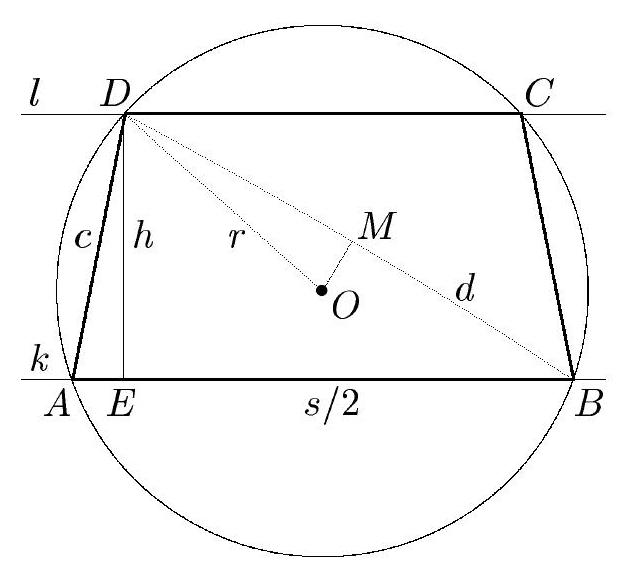
\includegraphics[max width=\textwidth, center]{2024_11_16_fe5b564401bf7db98894g-120}

Rys. 25\\
wód wynosi $O=s+2 c=s+\frac{16 P r}{\sqrt{16 P^{2}+s^{4}}}$. Dane $P$ i $s$ wyznaczaja jednoznacznie $h$ i $d$. Zadanie ma zatem rozwiązanie, gdy promień $r$ jest wystarczająco duży, aby powstał trójkạt $\triangle D O M$, tzn. $\quad r \geq \frac{1}{2} d=\frac{\sqrt{16 P^{2}+s^{4}}}{4 s}$. Poprawność tego warunku, jak i jednoznaczność rozwiązania, najlepiej widać z opisu konstrukcji trapezu, który dla kompletności przedstawiamy poniżej.

\section*{Opis konstrukcji trapezu}
\begin{enumerate}
  \item Z odcinków $h$ i $\frac{s}{2}$, jako przyprostokątnych, konstruujemy trójkąt prostokatny $D E B$. Odcinek $B E$ przedłużamy i otrzymujemy prosta $k$, a przez punkt $D$ prowadzimy prostą $l$ równoległą do $k$.
  \item Z punktów $B$ i $D$ kreślimy łuki okrẹgów o promieniu $r$, które przecinając się dają środek okręgu opisanego $O$ (z dwóch punktów, w których przecinają się te łuki, wybieramy leżący bliżej prostej $k$, która ma zawierać dłuższą podstawę trapezu).\\
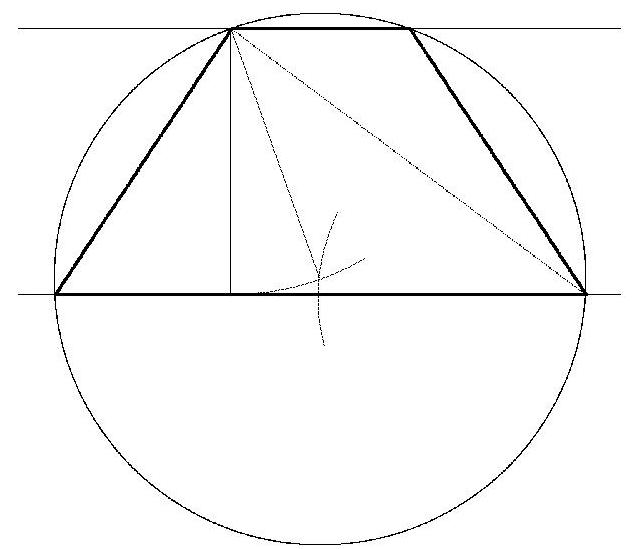
\includegraphics[max width=\textwidth, center]{2024_11_16_fe5b564401bf7db98894g-121}
\end{enumerate}

Rys. 26\\
3. Ze środka $O$ kreślimy okrąg o promieniu $r$. Okrag ten przecinajac prosta $k$, wyznacza wierzchołek $A$ (oraz przechodzi przez $B$ ). Podobnie, okrag ten przecinajac prosta $l$, wyznacza wierzchołek $C$ (i równocześnie przechodzi przez $D$ ). Na rysunku 26 przedstawiono konstrukcje trapezu dla danych liczbowych zadania, tj. $P=12 \mathrm{~cm}^{2}$, $h=3 \mathrm{~cm}$ i $s=8 \mathrm{~cm}$.

Odp. Obwód wynosi $s+\frac{16 P r}{\sqrt{16 P^{2}+s^{4}}}$, a zadanie ma rozwiązanie, gdy $r^{2} \geq \frac{P^{2}}{s^{2}}+\frac{s^{2}}{16}$.

\section*{Rozwiazanie zadania 21.7}
Logarytm jest określony dla liczb dodatnich, więc dziedzinę równania wyznaczaja warunki:

$$
D:\left\{\begin{array}{l}
1-x>0 \\
x+4>0 \\
x^{3}-x^{2}-3 x+5>0
\end{array}\right.
$$

czyli $D:(x \in(-4,1)) \wedge\left(x^{3}-x^{2}-3 x+5>0\right)$. W celu rozwiązania równania wszystkie składniki zapiszemy jako logarytmy o podstawie 4. Dla $x \in D$ jest $\log _{2}(1-x)=\frac{\log _{4}(1-x)}{\log _{4} 2}=2 \log _{4}(1-x)=\log _{4}(x-1)^{2}$ oraz $\frac{1}{2}=\log _{4} 2$ i równanie przyjmuje postać

$$
\log _{4}(x-1)^{2}+\log _{4}(x+4)=\log _{4}\left(x^{3}-x^{2}-3 x+5\right)+\log _{4} 2 .
$$

Korzystając z własności logarytmu oraz z różnowartościowości funkcji logarytmicznej, widzimy, że równanie (3) jest równoważne (w dziedzinie) równaniu algebraicznemu $(x-1)^{2}(x+4)=2\left(x^{3}-x^{2}-3 x+5\right)$. Po wykonaniu działań i przeniesieniu wszystkich składników na jedną stronę dostajemy

$$
x^{3}-4 x^{2}+x+6=0
$$

Pierwiastki całkowite równania (4) sa podzielnikami wyrazu wolnego, tj. liczby 6. Przez podstawienie sprawdzamy bezpośrednio, że liczby -1, 2 i 3 spełniają (4), czyli są wszystkimi pierwiastkami tego równania (mając dwa pierwiastki, np. -1 i 2 , trzeci można znaleźć z relacji $x_{1} x_{2} x_{3}=-6$ ). Liczby 2 i 3 znajdują się poza przedziałem $(-4,1)$, czyli leża poza $D$. Natomiast $-1 \in(-4,1)$ oraz $(-1)^{3}-(-1)^{2}-3(-1)+5=6>0$, czyli liczba -1 jest jedynym pierwiastkiem danego równania.

Odp. Równanie ma tylko jeden pierwiastek i jest nim liczba -1 .

\section*{Rozwiazanie zadania 22.7}
Dziedzinę równania określają warunki

$$
D:\left\{\begin{array}{l}
\sin x \neq 0 \\
\cos x \neq 0,
\end{array}\right.
$$

czyli warunki $x \neq k \pi$ oraz $x \neq \frac{\pi}{2}+k \pi$. To daje ostatecznie

$$
D: x \neq k \frac{\pi}{2}, \quad k \in \mathbf{Z}
$$

Dla $x \in D$ mnożymy obie strony równania przez $(\sin x \cos x)$ i otrzymujemy równanie równoważne

$$
\sin x+\cos x=\sqrt{8} \sin x \cos x
$$

Korzystając ze wzoru redukcyjnego oraz wzoru na różnicę cosinusów, mamy $\sin x+\cos x=\cos x-\cos \left(x+\frac{\pi}{2}\right)=-2 \sin \left(-\frac{\pi}{4}\right) \sin \left(x+\frac{\pi}{4}\right)$. Ponadto $\sqrt{8} \sin x \cos x=\sqrt{2} \sin 2 x$, zatem równanie (5), po podzieleniu obu stron przez $\sqrt{2}$, można zapisać w postaci

$$
\sin \left(x+\frac{\pi}{4}\right)=\sin 2 x
$$

\begin{center}
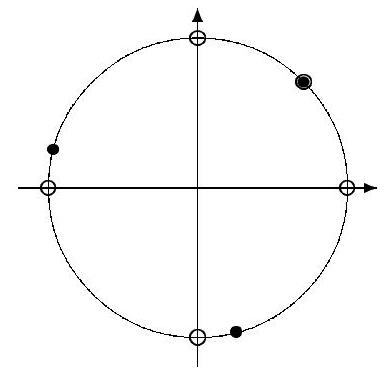
\includegraphics[max width=\textwidth]{2024_11_16_fe5b564401bf7db98894g-123}
\end{center}

Rys. 27

Stąd otrzymujemy alternatywę równań liniowych $x+\frac{\pi}{4}=2 x+2 k \pi$ lub $x+\frac{\pi}{4}=$ $\pi-2 x+2 k \pi$, gdzie $k \in \mathbf{Z}$. Po standardowych przeksztatceniach mamy $x=\frac{\pi}{4}+2 k \pi$ lub $x=\frac{\pi}{4}+k \frac{2 \pi}{3}$. Zauważmy, że pierwsza seria zawiera się w drugiej (rys. 27), a ta z kolei jest zawarta w dziedzinie równania.

Odp. $x=\frac{\pi}{4}+k \frac{2 \pi}{3}, \quad k \in \mathbf{Z}$.

\section*{Rozwiazanie zadania 26.4}
Oznaczmy przez $O$ spodek wysokości czworościanu, a przez $K, L$ jego rzuty prostokątne odpowiednio na przyprostokatne $B C$ i $A C$ podstawy (rys. 28). Ponieważ $O$ jest środkiem okrẹgu wpisanego w $\triangle A B C$, więc\\
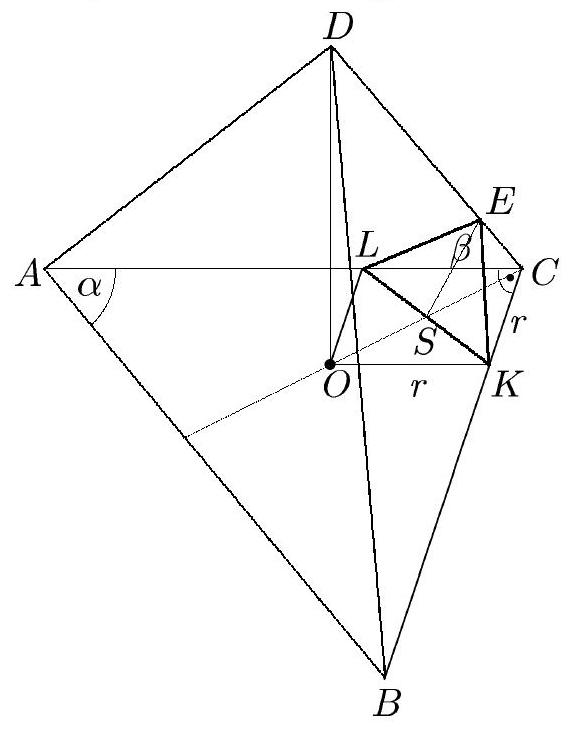
\includegraphics[max width=\textwidth, center]{2024_11_16_fe5b564401bf7db98894g-123(1)}

Rys. 28\\
$|O K|=|O L|=r$, czyli punkty $O, \quad K, \quad L$ i wierzchołek kạta prostego $C$ tworza kwadrat o boku $r$. Stąd

$$
|K C|=|L C| .
$$

Mamy $\triangle D O K \equiv \triangle D O L$, gdyż oba sa prostokatne i maja takie same przyprostokatne. Stąd $|D K|=|D L|$. Ponieważ wysokość $D O$ jest prostopadła do podstawy, więc $D O \perp B C$. Ponadto $O K \perp B C . \quad \mathrm{Z}$ twierdzenia o trzech prostopadłych wnioskujemy, że $D K \perp B C$. Analogicznie stwierdzamy, że $D L \perp A C$.\\
Wynika stąd, że $\triangle D K C$ i $\triangle D L C$ są przystającymi trójkatami prostokatnymi i w konsekwencji

$$
\angle D C K=\angle D C L
$$

Niech $E$ oznacza rzut prostokątny punktu $K$ na krawędź $D C$. Ze wzorów (6) i (7) oraz z II cechy przystawania trójkątów (bkb) wynika, że $\triangle K C E \equiv \triangle L C E$, a stąd $L E \perp D C$. To oznacza, że krawędź $D C$ jest\\
prostopadła do płaszczyzny wyznaczonej przez punkty $K, L$ i $E$ i w konsekwencji $\angle K E L=\beta . \mathrm{Z}$ porównania trójkątow równoramiennych $\triangle K C L$ i $\triangle K E L$, majacych wspólną podstawę oraz $|K E|<|K C| \quad(|K E|$ jest przyprostokątną), wnioskujemy, że $\angle K E L=\beta>\angle K C L=\frac{\pi}{2}$, zatem dziedziną dla kąta $\beta$ jest $\operatorname{przedziat}\left(\frac{\pi}{2}, \pi\right)$.\\
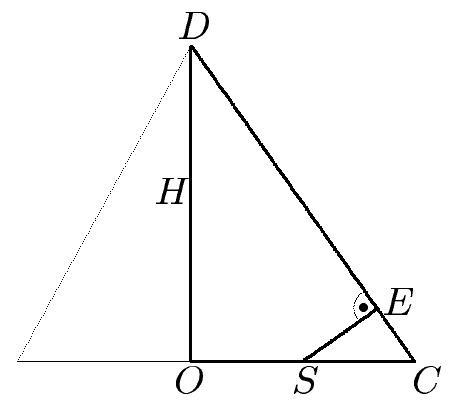
\includegraphics[max width=\textwidth, center]{2024_11_16_fe5b564401bf7db98894g-124}

Rys. 29\\
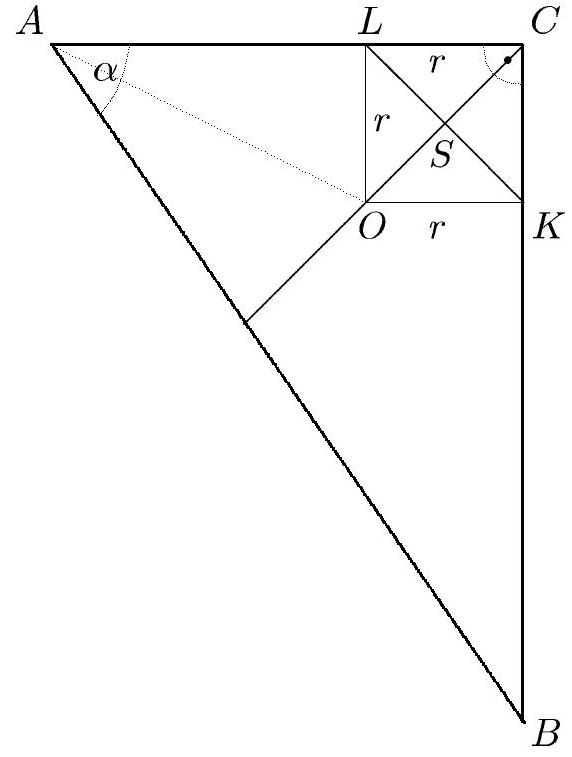
\includegraphics[max width=\textwidth, center]{2024_11_16_fe5b564401bf7db98894g-124(1)}

Rys. 30

W celu wyznaczenia wysokości czworościanu oznaczmy przez $S$ środek kwadratu $O K C L$. Wówczas $|E S|=|S K| \operatorname{ctg} \frac{\beta}{2}=\frac{r}{\sqrt{2}} \operatorname{ctg} \frac{\beta}{2}$. Poprowadźmy płaszczyznę przechodzącą przez $D O$ oraz przez $C$. Przekrój czworościanu tą płaszczyzna pokazano na rysunku 29. Z twierdzenia Pitagorasa w $\triangle E S C$ mamy $|E C|^{2}=|S C|^{2}-|E S|^{2}=\frac{r^{2}}{2}-\frac{r^{2}}{2} \operatorname{ctg}^{2} \frac{\beta}{2}=r^{2} \frac{-\cos \beta}{2 \sin ^{2} \frac{\beta}{2}}$. Z podobieństwa trójkạtów $\triangle E S C$ i $\triangle D O C$ dostajemy proporcje $\frac{H}{|O C|}=\frac{|E S|}{|E C|}$. Stąd

$$
H=\frac{|O C||E S|}{|E C|}=\frac{r^{2} \operatorname{ctg} \frac{\beta}{2}}{r \sqrt{\frac{-\cos \beta}{2 \sin ^{2} \frac{\beta}{2}}}}=r \sqrt{2} \frac{\cos \frac{\beta}{2}}{\sqrt{-\cos \beta}}
$$

Dla obliczenia pola podstawy czworościanu (rys. 30) zauważmy, że $|A C|=|L C|+|A L|=r+\operatorname{rctg} \frac{\alpha}{2}$ oraz $|B C|=|A C| \operatorname{tg} \alpha$. Stad mamy

$$
P_{p}=\frac{1}{2}|A C| \cdot|B C|=\frac{1}{2} r^{2}\left(\operatorname{ctg} \frac{\alpha}{2}+1\right)^{2} \operatorname{tg} \alpha=\frac{1}{2} r^{2} \frac{\left(\sin \frac{\alpha}{2}+\cos \frac{\alpha}{2}\right)^{2}}{\sin ^{2} \frac{\alpha}{2}} \operatorname{tg} \alpha
$$

i ostatecznie

$$
P_{p}=r^{2} \frac{1+\sin \alpha}{\cos \alpha} \operatorname{ctg} \frac{\alpha}{2} .
$$

Z równości (8) i (9) otrzymujemy

$$
V=\frac{1}{3} P_{p} H=\frac{\sqrt{2}}{3} r^{3} \frac{1+\sin \alpha}{\cos \alpha \sqrt{-\cos \beta}} \cos \frac{\beta}{2} \operatorname{ctg} \frac{\alpha}{2}
$$

Odp. Objętość czworościanu wynosi $\frac{\sqrt{2}}{3} r^{3} \frac{1+\sin \alpha}{\cos \alpha \sqrt{-\cos \beta}} \cos \frac{\beta}{2} \operatorname{ctg} \frac{\alpha}{2}$.

\section*{Rozwiazanie zadania 28.2}
Aby nierówność

$$
\frac{2 p x^{2}+2 p x+1}{x^{2}+x+2-p^{2}} \geq 2
$$

była spełniona dla każdej liczby rzeczywistej, jej dziedziną musi być R, czyli trójmian kwadratowy w mianowniku nie może mieć pierwiastków rzeczywistych. Stad otrzymujemy warunek $\Delta_{0}=1-4\left(2-p^{2}\right)=4 p^{2}-7<0$. Nierówność ta jest spełniona dla

$$
p \in\left(-\frac{\sqrt{7}}{2}, \frac{\sqrt{7}}{2}\right) .
$$

Dla parametru $p$ spełniajacego warunek (11) mianownik lewej strony (10) jest dodatni na całej prostej, więc po pomnożeniu obu stron (10) przez ten mianownik otrzymujemy nierówność równoważną $2 p x^{2}+2 p x+1 \geq 2 x^{2}+2 x+4-2 p^{2}$, a po uporządkowaniu

$$
2(p-1) x^{2}+2(p-1) x+2 p^{2}-3 \geq 0
$$

Dla $p=1$ lewa strona (12) jest równa -1 i nierówność nie jest spełniona dla żadnego $x$. Gdy $p<1$ tzn. współczynnik przy $x^{2}$ jest ujemny, nierówność (12) nie może być spetniona dla wszystkich $x$ (gdyż ,,ramiona paraboli sa skierowane w dół"). Natomiast dla $p>1$, nierówność (12) będzie spełniona dla wszystkich liczb rzeczywistych wtedy i tylko wtedy, gdy $\Delta_{1}=4(p-1)^{2}-8(p-1)\left(2 p^{2}-3\right) \leq 0$. Po podzieleniu obu stron przez wyrażenie dodatnie $4(p-1)$ otrzymujemy $-4 p^{2}+p+5 \leq 0$, skąd od razu mamy $p \leq-1$ lub $p \geq \frac{5}{4}$. Ponieważ $\frac{5}{4}<\frac{\sqrt{7}}{2}$ i założyliśmy, że $p>1$, więc łacczac wszystkie otrzymane warunki dostajemy ostatecznie $p \in\left[\frac{5}{4}, \frac{\sqrt{7}}{2}\right)$.

Odp. Nierówność jest spełniona dla każdej liczby rzeczywistej, gdy $p \in\left[\frac{5}{4}, \frac{\sqrt{7}}{2}\right)$.

\section*{Rozwiazanie zadania 29.8}
Z postaci ciagu odczytujemy wyraz początkowy $a_{0}=x+1$ oraz iloraz $q=-x^{2}$. Jeśli $x=-1$, to wszystkie wyrazy ciagu sa zerami i suma $S(-1)=0$. Gdy $x \neq-1$, wówczas warunkiem istnienia sumy nieskończonego ciagu geometrycznego jest $|q|<1$, czyli $\left|-x^{2}\right|=x^{2}<1$, skad od razu otrzymujemy $x \in(-1,1)$. Ostatecznie dziedzina sumy $S(x)$ jest $D=[-1,1)$.

Korzystając ze wzoru na sumę nieskończonego ciagu geometrycznego, dostajemy $S(x)=\frac{x+1}{1-\left(-x^{2}\right)}=\frac{x+1}{x^{2}+1}, \quad x \in(-1,1)$. Wzór ten pozostaje prawdziwy także dla $x=-1$. Dlatego można napisać

$$
S(x)=\frac{x+1}{x^{2}+1}, \quad x \in D=[-1,1)
$$

Dalsze postępowanie sprowadza się do wyznaczenia wartości namniejszej i największej funkcji wymiernej $S(x)$, danej wzorem (13). Zauważmy, że mianownik jest dodatni, a licznik nieujemny, zatem $S(x) \geq 0$ dla wszystkich $x$. Stąd wynika, że najmniejszą wartością tej funkcji jest 0 i jest ona osiagana dla $x=-1$.

Dla znalezienia wartości największej wykorzystamy pochodną funkcji $S(x)$.

$$
S^{\prime}(x)=\frac{1 \cdot\left(x^{2}+1\right)-2 x(x+1)}{\left(x^{2}+1\right)^{2}}=\frac{-x^{2}-2 x+1}{\left(x^{2}+1\right)^{2}} .
$$

Miejsca zerowe pochodnej spełniaja równanie $-x^{2}-2 x+1=0$. Stad dostajemy $\Delta=8$ oraz $x_{1}=-1-\sqrt{2}, x_{2}=-1+\sqrt{2}$. Tylko $x_{2} \in D$. Mamy $S\left(x_{2}\right)=\frac{\sqrt{2}}{1+2-2 \sqrt{2}+1}=\frac{1+\sqrt{2}}{2}$ oraz $\lim _{x \rightarrow 1^{-}} S(x)=\lim _{x \rightarrow 1^{-}} \frac{x+1}{x^{2}+1}=1$. Ponieważ $\frac{1+\sqrt{2}}{2}>1$, więc największą wartością funkcji jest $\frac{1+\sqrt{2}}{2}$.

Odp. Wartość najmniejsza sumy danego nieskończonego ciagu geometrycznego wynosi 0 i jest osiągana dla $x=-1$, a wartość największa tej sumy wynosi $\frac{1+\sqrt{2}}{2} \mathrm{i}$ jest osiagana dla $x=-1+\sqrt{2}$.

\section*{Rozwiazanie zadania 30.7}
Dziedzina nierówności

$$
\left|2^{x}-3\right| \leq 2^{1-x}
$$

jest $\mathbf{R}$. Nierówność tę rozwiążemy przez podstawienie $2^{x}=t, t>0$. Mamy $2^{1-x}=22^{-x}=2 \frac{1}{t}$, więc po podstawieniu nierówność (14) przyjmie postać $|t-3| \leq \frac{2}{t}$. Stąd od razu przechodzimy do nierówności podwójnej

$$
-\frac{2}{t} \leq t-3 \leq \frac{2}{t}, \quad t>0
$$

Ze względu na dodatni znak niewiadomej $t$ możemy tę nierówność pomnożyć przez $t$ i otrzymamy następujaçy układ nierówności kwadratowych

$$
\left\{\begin{array}{l}
t^{2}-3 t+2 \geq 0 \\
t^{2}-3 t-2 \leq 0
\end{array}, t>0\right.
$$

Pierwsza nierówność powyższego układu jest spełniona dla $t \leq 1 \mathrm{i} t \geq 2$, czyli po uwzględnieniu warunku $t>0$ dla $t \in(0,1] \cup[2, \infty)$. Dla drugiej nierówności mamy $\Delta_{2}=17, t_{1}^{\prime \prime}=\frac{3-\sqrt{17}}{2}<0, t_{2}^{\prime \prime}=\frac{3+\sqrt{17}}{2} \in(3,4)$. Druga nierówność jest zatem spełniona dla $t \in\left(0, t_{2}^{\prime \prime}\right]$. Część wspólna zbiorów rozwiązań obu nierówności ma postać ( $0,1\left[\cup\left[2, t_{2}^{\prime \prime}\right]\right.$. Ponieważ funkcja $t=2^{x}$ jest rosnąca, więc zbiór rozwiązań nierówności (14) ma postać $(-\infty, 0] \cup\left[1, x_{0}\right]$, gdzie $x_{0}=\log _{2} t_{2}^{\prime \prime} \in(1,2)$.

Wykresy funkcji występujących po obu stronach nierówności (14) otrzymujemy przez translacje i odbicia symetryczne standardowej krzywej $\Gamma: y=2^{x}$. Wykres krzywej $y=\left|2^{x}-3\right|$ dostajemy przez translację $\Gamma$ o wektor $[0,-3]$, a następnie odbicie symetryczne części leżącej pod osią odciętych względem tej osi. Krzywa ta ma asymptotę poziomą lewostronna $y=3$. Natomiast krzywa $y=2^{1-x}$ dostajemy przez odbicie symetryczne $\Gamma$ względem osi rzędnych, a następnie translację o wektor $(1,0)$. Wykresy sa przedstawione na rysunku 31.\\
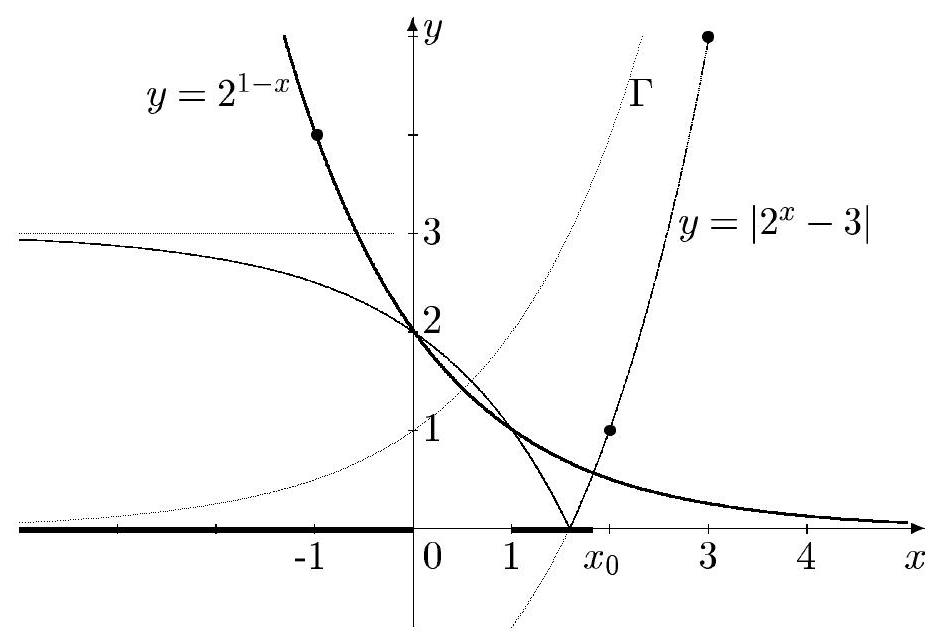
\includegraphics[max width=\textwidth, center]{2024_11_16_fe5b564401bf7db98894g-128}

Rys. 31\\
Odp. Zbiorem rozwiązań nierówności jest suma przedziałów $(-\infty, 0] \cup\left[1, \log _{2} \frac{3+\sqrt{17}}{2}\right]$.

\section*{Rozwiąanie zadania 31.7}
Przy rozwiązywaniu zadania skorzystamy następującej własności wektorów na płaszczyźnie:

Twierdzenie. Jeśli wektory $\vec{u} i \vec{v}$ sa prostopadte $i$ maja te sama dtugość oraz $\vec{u}=(a, b)$, to $\vec{v}=(b,-a)$ lub $\vec{v}=(-b, a)$.\\
Przez $B$ oznaczmy wierzchołek kwadratu leżacy na prostej $l$, a przez $D$ jego wierzchołek leżacy na prostej $k$. Korzystając z równań prostych, możemy napisać $B(2 y-1, y), \quad D(4-3 z, z)$, gdzie $y, z$ sa nieznanymi rzędnymi tych wierzchołków, zatem $\overrightarrow{A B}=[2 y-7, y-1]$ oraz\\
$\overrightarrow{A D}=[-3 z-2, z-1]$. Ponieważ $\overrightarrow{A B} \perp \overrightarrow{A D}$ oraz oba wektory są tej samej długości, więc z powyższego twierdzenia otrzymujemy z porównania odpowiednich współrzędnych dwa układy równań liniowych:

$$
\left\{\begin{array} { c } 
{ 2 y - 7 = - z + 1 } \\
{ - 3 z - 2 = y - 1 }
\end{array} \text { oraz } \left\{\begin{array}{l}
2 y-7=z-1 \\
3 z+2=y-1
\end{array} .\right.\right.
$$

Po rozwiązaniu pierwszego układu dostajemy $y=3, z=0$, czyli $B_{1}(5,3)$, $D_{1}(4,0)$ oraz $\overrightarrow{A B}=[-1,2]$. Ponieważ $\overrightarrow{A B}=\overrightarrow{D C}$, więc $C_{1}(3,2)$. Rozwiązaniem drugiego układu jest $y=5, z=-2$, czyli $B_{2}(9,5), \quad D_{2}(10,-2)$ i podobnie jak poprzednio $\overrightarrow{A B}=\overrightarrow{D C}=[4,-3]$, skąd $C_{2}(13,2)$. Rozwiązanie ilustruje rysunek 32.

Uwaga. Ze względu na ogólnie przyjęty sposób oznaczania wierzchołków wielokątów na rysunku 32 przestawiono litery $B$ i $D$, oznaczajac $B_{2}(10,-2)$ i $D_{2}(9,5)$.\\
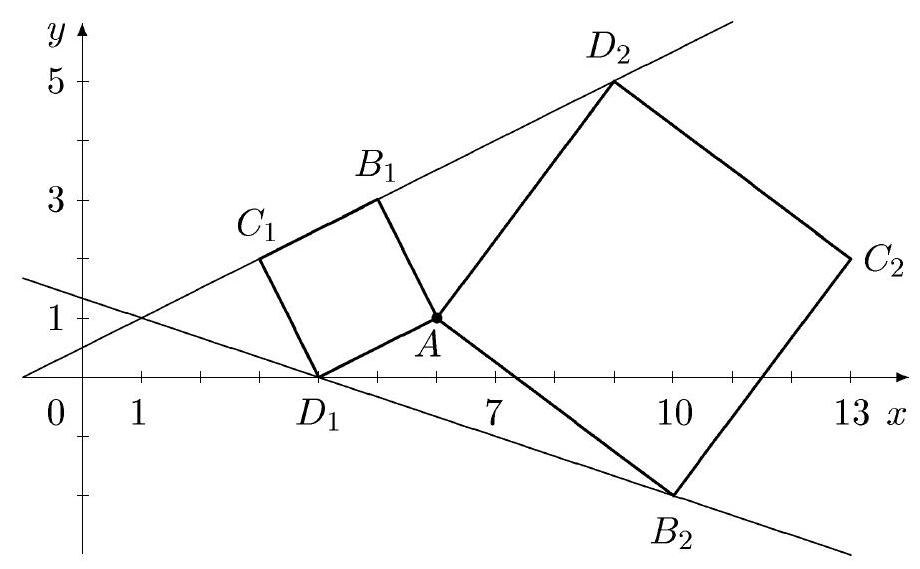
\includegraphics[max width=\textwidth, center]{2024_11_16_fe5b564401bf7db98894g-129}

Rys. 32\\
Odp. Istnieją dwa kwadraty spełniajace warunki zadania. Ich wierzchołkami, oprócz wierzchołka $A$, są punkty $B_{1}(5,3), C_{1}(3,2), D_{1}(4,0)$ oraz $B_{2}(10,-2), C_{2}(13,2), D_{2}(9,5)$.

\section*{Rozwiazanie zadania 32.7}
Równanie stycznej do wykresu funkcji $f(x)$ w punkcie $S\left(x_{0}, f\left(x_{0}\right)\right)$ ma postać ogólna $y-f\left(x_{0}\right)=f^{\prime}\left(x_{0}\right)\left(x-x_{0}\right)$. Ponieważ w naszym przypadku\\
jest $f(x)=x^{4}-2 x^{2}$ oraz $f^{\prime}(x)=4 x^{3}-4 x$, więc równanie stycznej przyjmie postać

$$
y-\left(x_{0}^{4}-2 x_{0}^{2}\right)=\left(4 x_{0}^{3}-4 x_{0}\right)\left(x-x_{0}\right)
$$

Punkt $P(1,-1)$ leży na tej stycznej, więc niewiadoma $x_{0}$ spełnia równanie $-1+2 x_{0}^{2}-x_{0}^{4}=4 x_{0}\left(x_{0}^{2}-1\right)\left(1-x_{0}\right)$. Po wyłaczeniu wspólnych czynników i uporządkowaniu dostajemy $\left(x_{0}^{2}-1\right)\left(x_{0}-1\right)\left(3 x_{0}-1\right)=0$. Równanie (16) ma więc trzy pierwiastki $-1,1$ oraz $\frac{1}{3}$.

Po podstawieniu do równania (16) pierwiastków $x_{0}=-1$ i $x_{0}=1$ otrzymujemy tę sama prostą $p: y+1=0$. Prosta ta jest wię styczna do wykresu $f$ równocześnie w punktach $P(-1,1)$ oraz $Q(-1,-1)$. Ponieważ $f(x)=x^{4}-2 x^{2} \geq-1\left(\operatorname{inaczej}\left(x^{2}-1\right)^{2} \geq 0\right)$ dla wszystkich $x$ i równość ma miejsce jedynie dla $x=-1$ i $x=1$, więc styczna $p$ ma dwa punkty wspólne z wykresem $f$.

Dla $x_{0}=\frac{1}{3}$ równanie (16) przyjmuje postać $l: 32 x+27 y-5=0$. W celu określenia liczby punktów wspólnych stycznej $l \mathrm{z}$ wykresem $f$ należy określić liczbę różnych pierwiastków równania $x^{4}-2 x^{2}=\frac{5-32 x}{27}$, tj. równania $27 x^{4}-54 x^{2}+32 x-5=0$. Ze względu na styczność w punkcie $x_{0}=\frac{1}{3}$ równanie to ma podwójny pierwiastek $\frac{1}{3}$ oraz pierwiastek 1 (punkt $P$ leży na wykresie $f$ ), zatem, jako równanie czwartego stopnia, ma także czwarty pierwiastek rzeczywisty, który obliczamy z równości $x_{1} x_{2} x_{3} x_{4}=\frac{-5}{27}$, czyli w naszym przypadku $\frac{1}{9} x_{4}=\frac{-5}{27}$, skąd $x_{4}=\frac{-5}{3}$. Styczna $l$ ma zatem trzy punkty wspólne z wykresem $f: P, S\left(\frac{1}{3},-\frac{17}{81}\right)$ oraz $A\left(-\frac{5}{3}, \frac{175}{81}\right)$. W punkcie $A$ styczna $l$ przecina wykres $f$. Dla sporzadzenia rysunku zauważmy, że $f(x)$ jest funkcja parzysta. Liczba $x=0$ jest pierwiastkiem podwójnym równania $x^{4}-2 x^{2}=0$, co oznacza, że wykres $f$ jest styczny do osi odciętych w poczatku układu. Pozostałe miejsca zerowe funkcji to $-\sqrt{2}$ i $\sqrt{2}$. Kreślac styczne $y=0, l$ oraz $p$ i zaznaczając punkty styczności oraz punkty $(\sqrt{2}, 0), B\left(\frac{5}{3}, \frac{175}{81}\right)$, możemy narysować wykres funkcji na $(0, \infty)$, a przez odbicie symetryczne także w $(-\infty, 0)$. Wykres przedstawiono na rysunku 33.\\
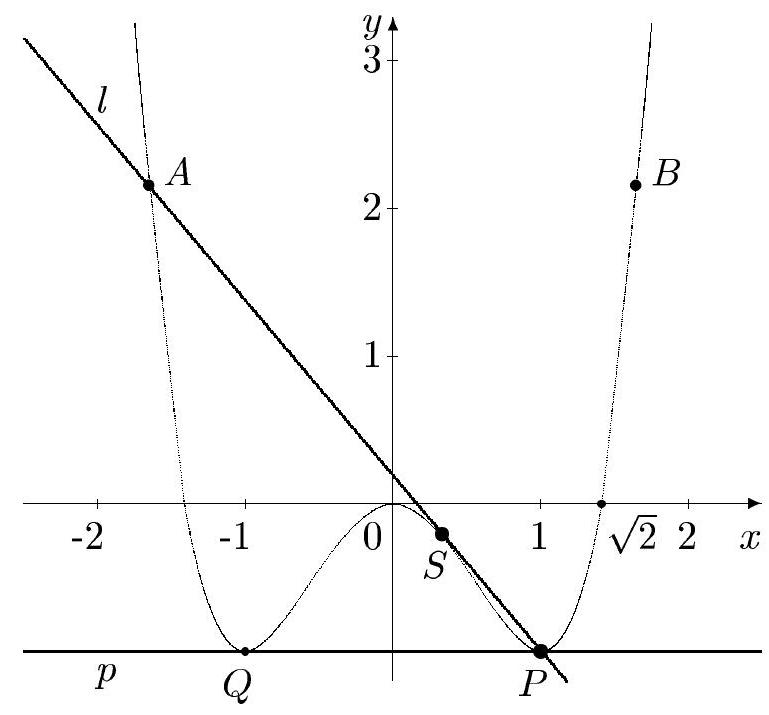
\includegraphics[max width=\textwidth, center]{2024_11_16_fe5b564401bf7db98894g-131}

Rys. 33\\
Odp. Sa dwie takie styczne jedna o równaniu $y=-1$, która ma dwa punkty wspólne z wykresem funkcji $f(x)$, oraz druga o równaniu $32 x+27 y-5=0$ majaca trzy punkty wspólne z wykresem.

\section*{Rozwiazanie zadania 34.5}
Wprowadźmy następujace zdarzenia:\\
$A$ - Jaś wyciagnie co najmniej trzy monety;\\
$B_{i}-$ za pierwszym razem zostanie wylosowana moneta o nominale $i \mathrm{zł}$, $i=1,2,5$;\\
$C_{j}-$ dla uiszczenia zapłaty Jaś wyciagnie $j$ monet, $j=1,2,3,4$.\\
Wówczas $A^{\prime}=C_{1} \cup C_{2}$ i oba składniki są rozłączne. Zauważmy, że $C_{1}=B_{5}$ oraz $B_{1} \cup B_{2} \cup B_{5}=\Omega$. Ponadto $P\left(B_{1}\right)=\frac{1}{2}, P\left(B_{2}\right)=\frac{1}{3}$ i $P\left(B_{5}\right)=P\left(C_{1}\right)=\frac{1}{6}$. Ze wzoru na prawdopodobieństwo całkowite mamy

$$
P\left(C_{2}\right)=P\left(C_{2} \mid B_{1}\right) P\left(B_{1}\right)+P\left(C_{2} \mid B_{2}\right) P\left(B_{2}\right)+P\left(C_{2} \mid B_{5}\right) P\left(B_{5}\right)
$$

Mamy $P\left(C_{2} \mid B_{1}\right)=\frac{1}{5}$, gdyż za drugim razem Jaś musi wyciagnaç monetę 5 zł spośród 5 monet w portmonetce. Podobnie $P\left(C_{2} \mid B_{2}\right)=\frac{2}{5}$ (za\\
drugim razem musi być wyciagnięta moneta 5 zł lub pozostała dostępna moneta 2 zl ) oraz $P\left(C_{2} \mid B_{5}\right)=0$ (nie ma drugiego losowania, gdy w pierwszym była moneta $5 \mathrm{zł}$ lub inaczej $C_{2} \cap B_{5}=\varnothing$ ). Po podstawieniu tych wartości do wzoru (17) dostajemy $P\left(C_{2}\right)=\frac{7}{30}$ i ostatecznie

$$
P(A)=1-P\left(C_{1}\right)-P\left(C_{2}\right)=1-\frac{7}{30}-\frac{1}{6}=\frac{6}{10}
$$

Odp. Prawdopodobieństwo tego, że Jaś wyciagnie co najmniej trzy monety wynosi $\frac{3}{5}$.


\end{document}